\documentclass[12pt]{article}
\usepackage{graphicx}
\usepackage{ragged2e}
\usepackage{times}

\usepackage[utf8]{inputenc}
\usepackage{subcaption}

\usepackage{amsmath}
\usepackage{booktabs}
\usepackage{blindtext}
\usepackage{enumitem}
%\usepackage{cmap}
\usepackage[T1]{fontenc}
\pagestyle{plain}
\usepackage{times}
\usepackage{amsmath}
\usepackage{geometry}
%\usepackage{sectsty}
%\usepackage{algorithmic}
%\usepackage{mathtools}
%\usepackage[titletoc,title]{appendix}
%\sloppy
%\usepackage[none]{hyphenat}

 \geometry{
 a4paper,
 total={155mm,242mm},
 left=35mm,
 top=35mm,
 }
%\usepackage{pdfpages}
%\usepackage{array}

\usepackage{titlesec}

\setcounter{secnumdepth}{4}
\setcounter{tocdepth}{4}


\titleformat{\section}
{\normalfont\large\bfseries}{\thesection.}{0.2em}{}

\titleformat{\subsection}
{\normalfont\normalsize\bfseries}{\thesubsection.}{0.2em}{}

\titleformat{\subsubsection}
{\normalfont\normalsize\bfseries}{\thesubsubsection.}{0.2em}{}

\titleformat{\paragraph}
{\normalfont\normalsize\bfseries}{\theparagraph.}{0.2em}{}
\titlespacing*{\paragraph}
{0pt}{3.25ex plus 1ex minus .2ex}{1.5ex plus .2ex}
% Uncomment for double-spaced document.

\renewcommand{\baselinestretch}{1.6}
%\sectionfont{\fontsize{14}{15}\selectfont}
%\subsectionfont{\fontsize{12}{15}\selectfont}
\makeatletter % access to internal commands
\renewcommand{\@seccntformat}[1]{\csname the#1\endcsname\ }
%\titlelabel{\thetitle.\quad}
\makeatother

% \usepackage{epsf}
\usepackage{chngcntr}
\counterwithin{figure}{section}
\counterwithin{table}{section}
\counterwithin{equation}{section}
\usepackage[parfill]{parskip}

\usepackage{fancyhdr}
\setlength{\headheight}{15pt}
\pagestyle{fancy}
\fancypagestyle{mystyle}{%
\fancyhf{}
\renewcommand{\headrulewidth}{0pt}
\fancyhead[R]{\thepage}}
\pagestyle{mystyle}

\usepackage{multicol}
\usepackage{times}
\usepackage{mathptmx}
\usepackage[unicode=true, pdfusetitle,
 bookmarks=true,bookmarksnumbered=false,bookmarksopen=false,
 breaklinks=false,pdfborder={0 0 0},backref=false,colorlinks=false]
 {hyperref}

\makeatletter
\numberwithin{equation}{section}

% we use this for our refernces as well
\AtBeginDocument{\renewcommand{\ref}[1]{\mbox{\autoref{#1}}}}

% redefinition of \equation for convenience
\let\oldequation = \equation
\let\endoldequation = \endequation
\renewenvironment{equation}{
\begin{oldequation}
}{
\end{oldequation}
\myequations{\@currentlabelname}
}

% try to make a List of Equations, 
% error is most likely in the @currentlabelname above
\usepackage{tocloft}
\newcommand{\listequationsname}{\Large List of Equations} 
\newlistof{myequations}{equ}{\listequationsname} 
\newcommand{\myequations}[1]{ 
\addcontentsline{equ}{myequations}{\protect\numberline{\theequation}#1}\par}
\setlength{\cftmyequationsnumwidth}{3em}

\makeatother

\usepackage{amssymb}
\usepackage{relsize}
\usepackage{hyperref}
\hypersetup{colorlinks=true}
\hypersetup{pdfborder={0 0 0}}
%\usepackage{tikz}
\usepackage[utf8]{inputenc}
 \setlength{\arrayrulewidth}{1mm}
\setlength{\tabcolsep}{18pt}
\renewcommand{\arraystretch}{1.5}
\usepackage{ragged2e}
\usepackage{chngcntr,tocloft}
\counterwithin*{figure}{section}
\counterwithin*{figure}{subsection}
\counterwithin*{figure}{subsubsection}

\addtolength{\cftfignumwidth}{2em}


\renewcommand{\thefigure}{%
  \ifnum\value{subsection}=0
    \thesection.\arabic{figure}%
  \else
    \ifnum\value{subsubsection}=0
      \thesubsection.\arabic{figure}%
    \else
      \thesubsubsection.\arabic{figure}%
    \fi
  \fi
}
%\usepackage{pstricks}
\usepackage{graphicx}
\usepackage{tabu}






\author{Pranish Bhagat}
\begin{document}
\pagenumbering{roman}
%==========coverpage===============
\begin{center}
 \vspace*{-3.0cm}
 

\includegraphics[width = 30mm]{logo.jpg}\\ [1.5mm] 

 TRIBHUVAN UNIVERSITY\\
        INSTITUTE OF ENGINEERING\\
        PULCHOWK CAMPUS\\
 \vspace{1.0cm}
 
 \center
		\textbf{\Large SWARM INTELLIGENCE BASED MAZE SOLVER}\\[2cm]
		
		 \center
		By:\\[2mm]
		\textbf{\large Digya Acharya (069BEX412)\\
		\large Pranish Bhagat (069BEX425)\\
		\large Pratik Bhandari (069BEX427)\\
		\large Sijan Bhattarai (069BEX438)}\\
    \vspace{2cm}
    
    \center
			 A PROJECT SUBMITTED TO THE DEPARTMENT OF ELECTRONICS AND COMPUTER ENGINEERING IN PARTIAL FULFILLMENT OF THE REQUIREMENT FOR THE BACHELOR'S DEGREE IN ELECTRONICS $\&$ COMMUNICATION ENGINEERING\\[1.5cm]
\center 
DEPARTMENT OF ELECTRONICS AND COMPUTER ENGINEERING
\center LALITPUR, NEPAL\\[1cm]
\center \today
	
 \end{center}
\thispagestyle{empty}
\newpage
\vfill
%=============acceptancepage===========
%\input{theacceptletter.tex}
%\vfill
%\newpage
%
%==============copyright=================
\section*{COPYRIGHT}
\justify 
The authors have agreed that the Library, Department of Electronics and Computer
Engineering, Central Campus, Pulchowk, Institute of Engineering may make this report
freely available for inspection. Moreover, the author has agreed that permission for extensive
copying of this project report for scholarly purpose may be granted by the supervisors who
supervised the project work recorded herein or, in their absence, by the Head of the
Department wherein the project report was done. It is understood that the recognition will
be given to the author of this report and to the Department of Electronics and Computer
Engineering, Central Campus Pulchowk, Institute of Engineering in any use of the material
of this project report. Copying or publication or the other use of this report for financial gain
without approval of to the Department of Electronics and Computer Engineering, Central
Campus Pulchowk, Institute of Engineering and author’s written permission is prohibited.\\
\\
Request for permission to copy or to make any other use of the material in this report in
whole or in part should be addressed to:\\[2cm]
\begin{flushleft}
Head of Department\\
Department of Electronics and Computer Engineering,\\
Institute of Engineering, Central Campus, Pulchowk,\\
Tribhuvan University, Nepal\\
\end{flushleft}
\vfill
\newpage
%============acknowledgement==============
\section*{ACKNOWLEDGEMENT}
We would like to express our deepest gratitude to the Department of Electronics and Computer Engineering, Institute of Engineering, Central campus for providing the opportunity for to work on Major Project as a part of our syllabus.\\
We are heartily indebted to our supervisor Mr.Dinesh Baniya Kshatri , for his constant support, critic and guidance throughout the project. It was his consistent suggestion that helped us to disentangle the obstacles encountered during the development of project.\\
We are grateful to the Head of Department of Electronics and Computer Engineering, Institute of Engineering, Pulchowk Campus, Assistant Professor, Dr. Dibakar Raj Pant, for his guidance and support.  \\
It would be injustice without acknowledging Dr. Nanda Bikram Adhikari  for the initial guidance in our project and for his motivation that encouraged us to put even more effort in the project. \\
 We would like to express my gratitude to the teachers of Institute of Engineering (IOE) who have helped and guided me directly or indirectly. Also, we would like to thank our friends and colleagues for their valuable comments and suggestions during the development of the project.\\ [1cm]
\begin{flushleft}
Digya Acharya (069BEX412) \\
Pranish Bhagat(069BEX425) \\
Pratik Bhandari (069BEX427) \\
Sijan Bhattarai (069BEX438)\\[5 mm]
(\today)\\ 
\end{flushleft}


\vfill
\newpage
%-------------------------------------------------------------

\section*{ABSTRACT}
\justify 
This project describes a multi-robot system designed to use Bluetooth wireless communication to solve the “Honeybee” task. The Honeybee task is a simple search and navigation problem that requires a “guide” robot to lead another “blind” robot to a specific target within the environment. Topics discussed include advantages and disadvantages of using Bluetooth in robotics, as well as a variety of behaviors required to solve the Honeybee task.\\
This project aims to implement and display the concept of swarm intelligence. Swarm intelligence is closely tied up with the Honeybee Problem described above. When two or generally more than two robots of similar or varying complexity work together in harmony to complete a single task or objective, where each robot does not necessarily perform the same task, swarm intelligence is said to be implemented. Various constraints such as budget and availability of resources prevented us from implementing swarm concept using more than two bots. Hence, only two bots of varying complexities are used in this project.
\subsection*{Keywords}
 Bluetooth, Maze Solving, Swarm Intelligence, Swarm Robotics \\

\vfill
\newpage
%---------------------------------------------------------------
\tableofcontents
\vfill
\newpage
\listoffigures
\vfill
\newpage
\listoftables
\vfill
\newpage
\listofmyequations
\vfill
%-----------------------------------------
\section*{LIST OF ABBREVIATIONS}
\begin{description}[align=left,labelwidth=3cm]
\item[AC] Alternating Current
\item[ACL] Asynchronous Connectionless
\item[ADC] Analog to Digital Converter
\item[AFH] Adaptive Frequency Hopping
\item[ARM] Advanced RISC Machine
\item[AT] Attention Commands
\item[BFS] Breadth-first search
\item[bps] bits-per-second
\item[CMOS] Complementary Metal–Oxide–Semiconductor 
\item[COP] Computer Operating Properly
\item[CPU] Central Processing Unit
\item[DC] Direct Current
\item[DECT] Digital Enhanced Cordless Telecommunications
\item[EEPROM] Electrically Erasable Programmable Read Only Memory
\item[EDR] Enhanced Data Rate
\item[GFSK] Gaussian Frequency Shift Keying
\item[GHz] GigaHertz
\item[GND] Ground
\item[IC] Integrated Circuit
\item[ICC] Instantaneous Center of Curvature
\item[ICSP] In-Circuit Serial Programming
\item[IDE] Integrated Development Environment
\item[IEEE] Institute of Electrical and Electronics Engineers
\item[I/O] Input Output
\item[IR] InfraRed
\item[ISM] Industrial, Scientific and Medical
\item[ISP] In-system Programming
\item[KB] KiloByte
\item[LC] Link Control
\item[LCD] Liquid Crystal Display
\item[LED] Light Emitting Diode
\item[LiPo] Lithium Polymer
\item[LPG] Liquefied Petroleum Gas
\item[mA] milli Ampere
\item[MHz] MegaHertz
\item[MIPS] Millions of Instructions
per second 
\item[mm] millimetre
\item[PAN] Personal Area Network
\item[PCB] Printed Circuit Board
\item[PIC] Programmable Intelligent Computer
\item[PIO] Programmed Input/Output
\item[PWM] Pulse Width Modulation
\item[QFP] Quad Flat Package
\item[RAM] Random Access Memory
\item[RF] Radio Frequency
\item[RISC] Reduced Instruction Set Computing
\item[ROM] Read Only Memory
\item[Rx] Receiver
\item[SAR] Search And Rescue
\item[SCO] Synchronous Connection-Oriented
\item[SIG] Special Interest Group
\item[SPP] Serial Port Protocol
\item[SRAM] Static Read Only Memory
\item[TTL] Transistor-Transistor Logic
\item[Tx] Transmitter
\item[UART] Universal Asynchronous Receiver/Transmitter\item[UHF] Ultra High Frequency
\item[USART] Universal Synchronous/Asynchronous Receiver/Transmitter
\item[USB] Uniform Serial Bus
\item[Vcc] Common Collector Voltage
\item[WDT] WatchDog Timer
\end{description}



\newpage
%\input{symbolpage.tex}
\newpage
%========================================
\pagenumbering{arabic}
\section{INTRODUCTION}
The purpose of this project is to design a multi-robot system which solves a simple maze using short range bluetooth communication. The project aims to create a robust communication system between two robots that would allow for the transmission of maze information from one maze-traversing bot to the other. \\
Although wireless communication protocols are relatively commonplace in the field of robotics, the use of this technology for coordinated robotics is somewhat different. Thus, the main contribution of this project is to outline the details of using wireless communication for coordinated swarm robotics.
Swarm robotics offers an intriguing approach to many real-world engineering problems. Such tasks that require covering a large search space or that involve working in potentially hazardous environments naturally lend themselves to robotic and swarm solutions. In many cases, autonomous robots can be the best option for a specific mission. Unmanned autonomous robotic vehicles which can enter the collapsed builds searching for survivors maybe a solution of finding survivors faster and safer. Being equipped with the necessary sensory devices, unmanned autonomous robotic vehicles can scan the environment sending precious information to the rescue teams about the location of survivors.\\
We have developed a multi-robot system designed to use short range wireless communication (Bluetooth) to solve a simple maze. A Maze Solving robot also known as a 'Micro-Mouse' robot is an autonomous vehicle which uses simple sensors to solve a maze without any human intervention. Maze-solving, although artificial in terms of the confine that the robot it subjected to, is a structured technique and controlled implementation of autonomous navigation. The choice of algorithms was limited to ones that required direct bot-to-bot communication and using bots with a limited sensing range. The Left Wall Follower Algorithm was implemented on the first bot, in the process showing the advantages and weakness of this technique. The bot will use data from simple obstacle-avoiding IR sensors to traverse through the maze whilst following the left wall. A maze, the complexity of which can be changed by moving its walls within the maze boundary will be used to test the system. Unlike in 'Micro-Mouse' systems, the destination of the maze will be unknown to the bot. Using suitable sensors, the first bot will reach the destination upon which it will transfer the maze information to the second bot. Hence, the second bot will traverse the maze based on the information provided by the first bot. 
Based on the robot reaching the target at the beginning, the shortest path to the target/destination will be calculated. The second bot will traverse the maze in the hence calculated shortest path.\\
Using the Arduino Uno chipset to program both the bots, the concept of swarm  robotics is well established in the project. The communication between two bots, one having higher complexity makes it easier for the other bot to be implemented with a lower complexity grade and still make it more intelligent. This concept can be well visualized in areas of emergence where a single vehicle cannot fulfill the task as effectively as a swarm of communicating bots can. The second bot and any other further bots that may/can be implemented in the system will inherently require less hardware and will always solve the maze in the shortest and most optimum path. This is the gist of swarm robotics. 
The concept of maze solving can be implemented in various real life situations as well. Natural disaster zones, hostage rescue situations, navigation in unknown territory are some examples. The left wall algorithm is one of the simplest and efficient methods to solve a maze. While moving through a maze it always follows the left wall, in meaning that at a junction it gives the most priority to the left turn. Future implementations of this algorithms might include a hybrid wall follower algorithm that implements both the left and right wall algorithms intelligently. Wireless communication using bluetooth technology allows the two bots to be completely devoid of human involvement during it's time of operation. Establishment of a communication pathway between two Arduinos using a bluetooth module is considered to be a significant milestone for the project. \\
Further topics following this will present the project and its method in a much greater detail and provide better insight into the technology implemented to achieve the project goal.


\subsection{Background}
In robotics, autonomous navigation is an important feature because it allows the robot to independently
move from a point to another without human intervention. Autonomous navigation within an unknown
area requires the robot to explore, localize and map its surrounding.\\
By solving a maze, the pertaining algorithms and behavior of the robot can be studied and
improved upon.\\
Swarm robotics is a new approach to the coordination of multirobot systems which consists
of large numbers of mostly simple physical robots. It is supposed that a desired collective
behavior emerges from the interactions between the robots and interactions of robots with
the environment. This approach emerged on the field of artificial swarm intelligence, as well
as the biological studies of insects, ants and other fields in nature, where swarm behavior
occurs.\\
Maze-solving is a structured technique and controlled implementation of autonomous navigation which
is sometimes preferable in studying specific aspect of the problem. These
robots are also known as “micro-mouse” robots. Research on various algorithms to efficiently
solve complex mazes has been ongoing since the past 50 years.\\
One of the most amazing developments in biological evolution is the domain of social insects. These
animals, although being very small, achieve impressive feats. Bees, ants and
termites live in elaborately constructed nests which are, in comparison to the insect, gigantic. The
colony super-organism can be characterized as being swarm-intelligent because its
abilities, for example to optimally allocate foragers to food sources, are a result of the interactions
within the swarm and cannot be achieved by the single individual. This decentralized
and distributed way of achieving a goal is an interesting and useful field of study which has
inspired the fields of swarm-intelligence and swarm robotics. In the last decade, a lot of
control strategies and algorithms for robotic swarms have been presented, both in simulated
and real robot swarms.\\
Maze-solving can be achieved using various sensing methods. For the robot to traverse the unknown
surrounding and identify obstacles successfully, it needs the help of certain sensors. IR sensors and
ultrosonic sensors have been widely used in such robots. Among them, IR sensors are more widely
used because of their narrow range of field whereas ultrasonic sensors have a wider sensing area. Light
Detection and Ranging (LiDAR) is another technology that has seen recent developments in use for
autonomous navigation. It is a surveying technology that measures distance by illuminating a target
with a laser light.\\
Bluetooth is a wireless technology standard for exchanging data over short distances (using
short-wavelength UHF radio waves in the ISM band from 2.4 to 2.485 GHz) from fixed and
mobile devices, and building personal area networks (PANs). Invented by telecom vendor
Ericsson in 1994,it was originally conceived as a wireless alternative to RS-232 data cables.
It can connect several devices, overcoming problems of synchronization but the bluetooth
module namely HC-05 used in our project is only able to connect to a single device i.e. a
single HC-05 is able to connect to another HC-05 or a personal computer wirelessly.
Bluetooth is managed by the Bluetooth Special Interest Group (SIG), which has more than
25,000 member companies in the areas of telecommunication, computing, networking, and
consumer electronics. The IEEE standardized Bluetooth as IEEE 802.15.1, but no longer
maintains the standard. The Bluetooth SIG oversees development of the specification, manages the qualification program, and protects the trademarks. A manufacturer must make a
device meet Bluetooth SIG standards to market it as a Bluetooth device.
\subsection{Problem Statement}
Swarm bots is a promising technology in recent robotics. But the construction of these bots is
complicated and tedious. We plan to design two swarm bots for solving a maze efficiently and in the
shortest possible path. Using a single robot creates difficulty in analyzing the shortest path. Moreover,
when multiple bots have to reach the same destination, it is faster with swarm-intelligence
implementation rather than multiple bots solving the maze independently.\\
The efficiency of the maze solving is boosted by the communication between the bots. The idea behind
swarm intelligence is reflected when two or more bots communicate with each other. With the age old
implementation of using single robots to solve a task, the process would not only be time consuming
but also less effective. Using multiple communicating bots greatly reduces the workload required on a
single bot and at the same time makes the entire process much more effective. For a task as simple as
solving a maze, a single robot would take multiple wrong turns and reach dead ends until it finally
reaches the target. When more than one robot is allowed to solve the maze in an integrated fashion, one
robot can work on one task while the other can work on another. For example, one can detect the target
while the other can decode the shortest path to it. With such communicating entity in place, the
underlying complexity for each bot is greatly reduced.\\
Maze solving alone is a much studied topic in robotics. The real world field of applications
implementing maze solving is quite diverse. Scenarios such as emergency evacuation in disaster
stricken areas require autonomous devices to traverse several obstacles to reach the destination which
might or might not be known firsthand. Similarly, in hostage rescue situations where the lives of not
only the hostages but also the rescuers matter equally, it is highly advisable to use such robots.
Unknown path finding and localization also implement maze solving techniques and algorithms.
Due to the lack of methods and tools, swarm robot designers cannot achieve the complexity required
for the real world applications. This project is just the small simulation in real world. The developed
swarm robot approach uses decentralized control strategies within the swarm of heterogeneous robots.
The robot-to-robot and robot-to-environment interaction provides the task oriented, simple collective
swarm behavior. We have decided to control the robot based on differential kinematics rather than
forward and inverse kinematics. This is done to avoid slippage, collision and cost. DC motors will be
used rather than stepper motors because of the speed limitation in the later one. IR sensors will be used
to detect the obstacles in the maze where the information received by these sensors will be used to
calculate the shortest path to the destination. The destination will be initially unknown and a smoke
sensor will be implemented to detect the target where a source of smoke will be placed. Arduino
microcontroller will be the brain of the robot where bluetooth technology will be used to establish a
communication link between the two robots. Hence, the advantages and application of swarm
intelligence is aimed to be demonstrated through successful implementation of this project.
\subsection{Motivation}
The idea behind our final year project came from the concept of ‘Swarm Robotics’. This
is a branch of robotics which is still in its infancy. Swarm robotics is the study of coordination of large
groups of relatively simple robots through the use of local rules. It takes its
inspiration from societies of insects that can perform tasks that are beyond the capabilities of
the individuals. Beni\cite{beni}, scholar, University of California describes this kind of robots’ coordination as follows:
”The group of robots is not just a group. It has some special characteristics, which are
found in swarms of insects, that is, decentralized control, lack of synchronization, simple
and (quasi) identical members.”\\
We want to demonstrate this concept using two robots which navigate their way through a
maze. The first bot will solve the maze individually taking as much time as it requires to reach an
unknown destination. The second one after communication with the first bot will solve the same maze
in the shortest path possible. While our project implements just two robots, any further robot that is
added to the system will solve the maze in the shortest path as well.\\
Our motivation arises from the behavior of insects such as ants which behave in a coordinated manner
and coordinating a group of robots in similar ways can ultimately make the
completion of any task simpler and less time consuming. Aside from this, we wanted to
implement a simple maze solving algorithm which can be implemented with minimal hardware
requirements keeping in mind the constraints in availability of materials in the local market.
Among the various methods to establish a communication link between the two robots, bluetooth
technology was chosen for its simplicity and ease of use within a short range.\\
Furthermore, in order to further justify the concept of swarm robotics we wanted to implement a simple
sensing circuitry. IR sensors were used as a result. With the use simple sensors and a simple algorithm
to traverse the maze and find the shortest path, we wanted to lay a foundation on the idea of swarm
intelligence upon which further additions could be done.\\
An advanced and real world use of our project which fueled our motivation to strive forward
with this idea was to implement this concept in Search and Rescue (SAR) operation, Land-mine
Detection, Hostage Rescue situations, etc. With slight modifications, mainly to the
mechanical parts and components, our project can be extended to a much larger and complex scale.
This turned out to be one of the most prominent sources of our motivation.
\subsection{Scope of Work}
Our final year project entitled “Swarm Intelligence Based Maze Solver” aims to develop and simulate the swarm concept in robotics by assigning specific tasks to each of the robots. The project is designed to develop a system of inter-communicating robots using the concept of swarm robotics. The primary objective of the first robot will be to solve a given maze and detect a target, namely smoke, within the maze whose location is unknown. Initially,  a single robot shall traverse the entire maze and shall detect the target. The map produced by the first robot shall be decoded and the effective shortest path will be transmitted to the  another robot via Bluetooth.Finally, the second robot traverses the shortest possible path   upto the target.\\
From this project, the idea of swarm robotics can be explained and verified. Using robust maze solving algorithms and precise communication technique methods the various objectives of our project will be fulfilled. Developing a robot which autonomously navigates its way through a maze and successfully detects a target is one of the many objectives of our project. Along with that, establishing a sound and secure communication link between two robots is another equally important objective of our project.
\subsection{Objectives}
The primary objective of our project is:
\begin{itemize}
\item To solve a maze  using the concept of swarm intelligence 
\end{itemize}
\justify To  achieve the primary objective, we need to fulfill the following secondary objectives:
\begin{itemize}
\item To implement small scale swarm robotics for maze solving.
\item  To implement wireless communication via Bluetooth for coordinated search.
\end{itemize}
 



\newpage
%==============================================================
\section{LITERATURE REVIEW}
While solving a maze using swarm intelligence is something that has not been
researched much, swarm intelligence and maze solving separately are not new topics
entirely.\\
Maze solving robots are more generally known as “Micromouse” and various models
of such robots implementing a variety of algorithms have been developed till date.
One of the first versions was developed by the University of East London. This
version of Micromouse\cite{micromouse} was developed by Michael Gims, Sonja Lenz and Dirk Becker
from University of East London in year 1999. The design of the mobile robot is quite
compact, but there is some improvement on the wiring. The algorithm applied is
\textbf{Wall Following Algorithm}. No past work has been done by the university
students in this particular field.\\
In the last two decades, theoretical research on multi-robot systems has been fueled by technological advances that now allow building relatively cheap small robots. An early categorization of multi-robot systems is given by Dudek et al\cite{second}, who identified swarm size, communication range, communication topology, communication bandwidth, swarm reconfigurability, swarm unit processing ability and swarm composition as taxonomy axes to classify natural or engineered multiagent systems.\cite{third}\\
The fundamental notion of cooperation between robots plays a central role in determining whether a multirobot system performs better than equivalent single-robot systems, and as such has been discussed in a number of exist-ing surveys. For example, cooperation is the central topic in\cite{fourth}, where swarm robotics systems are analyzed in terms of group architecture of the swarm (indicating with this term properties such as centralization versus decentralization,homogeneity versus heterogeneity, direct or indirect communication between agents, and how agents model each other), interference problems due to sharing of common resources, origin of cooperation (with interesting examples of how cooperation can be achieved implicitly even if each agent acts to maximize its individual utility), and learning mechanisms (with focus on reinforcement learning and genetic algorithms); in addition, a number of studies are grouped under the category of geometric problems, such as multiple-robot path planning and formation and marching problems. Iocchi et al.\cite{sixth}used cooperation as the first level of a multilevel characterization of robot swarms; cooperative systems are then further differentiated at the knowledge level, where systems with robots aware of the existence of other robots are distinguished from systems where each robot acts as if it was alone. The lower levels of the proposed taxonomy are the coordination level, describing how the actions of each robot take into ac-count the actions of other robots, and the organization level, which determines whether decisions are taken in a centralized or distributed way; it is interesting to note that a centralized system may be compatible with swarm intelligence principles: more precisely, systems defined as weakly centralized, where one of the robots temporarily assumes the role of leader, can exhibit the desired property of fault tolerance provided that suitable mechanisms are in place to assign the leadership role.\\
While early papers provided characterization of swarm robotics systems mainly as an analysis tool to encourage further research and give guidance for the design of new systems, with the increasing number of published studies describing actual implementations of robot swarms, newer surveys have been able to propose taxonomies where each category is represented by several examples of existing works. An extensive review of the state of the art in the mid 2000s is provided in A review of studies in swarm robotics, TurkishJournal of Electrical Engineering\cite{seventh}, where existing works are categorized based on analytical modeling approaches, design of individual robot behavior, type of interactions between robots, and problems being addressed by a robotic swarm. Gazi and Fida\cite{eighth} focused on the aspect of controlling robot movement, dividing existing works based on how the robot dynamics is modeled (i.e. how control inputs map to position variations) and how robot controllers are engineered; in addition, a further classification is done on the problem dimension. Previous works have been classified on the problem dimension also in other surveys; Mohanand Ponnambalam\cite{eleven} analyzed various research domains in swarm robotics,however their review does not provide a clear categorization of the state of the art, mixing a classification of some studies in the problem dimension with a description of how other studies differ on aspects such as biological inspiration,communication between robots, control approach and learning.\\
A comprehensive survey recently published is the work by Brambilla et al.\cite{twelve}, who proposed two taxonomies for swarm robotics studies: methods and collective behaviors. The first taxonomy includes design methods, differentiated in behavior-based and automatic methods, and analysis methods, i.e. techniques to study the performance of a swarm in executing a given task; analysis methods are divided in microscopic models, macroscopic models and real-robot analysis.The second taxonomy is based on the concept of collective behaviors, i.e. behaviors of a swarm of robots considered as a whole; the main categories identified by the authors under this taxonomy are spatially organizing behaviors, navigation behaviors and collective decision making.\\
Barca and Sekercioglu\cite{thirteen} analyzed past research by identifying a series of challenges faced by swarm robotics systems and describing how each of these challenges has been addressed by existing studies. Challenges are grouped under five categories: selecting appropriate communication and control schemes,incorporating self-organization, scalability and robustness properties, devising mechanisms to support goal-oriented formations, control and connectivity, implementing functions that enable robots to interact efficiently with the environment, and addressing problems related to energy consumption. The authors outlined a number of issues that need to be tackled to overcome these challenges,and observed how existing works typically focus on only a subset of these issues,suggesting that in order to implement successfully a swarm robotics system in real-world applications a larger set of issues should be tackled simultaneously.In this review, the problem dimension is used as main taxonomy axis, thus grouping past works according to the collective task being addressed. For each of the most studied tasks, first the main high-level methods employed in past studies are described, then task-specific categories are identified and a more detailed description of distributed algorithms is provided for a representative set of existing works in each category, and finally mathematical models to analyze and predict swarm behavior, and methods and metrics to evaluate swarm-level performance are reviewed. Due to similarities and analogies between different collective tasks, multiple equally valid categorizations can and have been proposed in past reviews under this taxonomy, and many works can be put in more than one category; in this study, partially different categories are identified compared to existing reviews, further categorizations within each task are proposed,and differences, similarities and relationships between tasks are explained.
In 2004, Quentin Chatelais, 
Horatiu Vultur and 
Emmanouil Kanellis of Aalborg University designed a maze solving autonomous robot. In their work, they focused on various topics such localization, mapping and path planning. In this project, much of this will not be implemented. \\
In 2012, Ibrahim Elshamarka and Abu Bakar Sayuti Saman of Universiti Teknologi PETRONAS designed a robot for maze-solving using Flood-Fill Algorithm. There are four main steps in the algorithm: Mapping, Flooding, Updating and Turning. The maze was divided into cells of equal size for the mapping of the region. Using suitable distance sensors, the map was updated with the information about the walls. \\
In terms of swarm intelligence, researches are still ongoing with recent developments
in this field. A combined research by various professors from different universities studies the architecture, protocols and applications of robot swarm communication.
This communication is built by constructing a wireless mesh network where one or
more robots get connected to nearby mesh router and access the remote server.
Combination of these two concepts have been implemented by students of Harvard
University. In this work, the robots traverse the map using wall following algorithm
and special pheromones are used by the bots to communicate with one another.
Another research by professors of University of Cincinnati explore various
algorithms for maze explorations for multi-agent systems using autonomous robots.
Another paper by Thomas Campbell of the Institute of Engineering at Murray State
Engineering studies the effect the maze-robotic size has on maze solving. He discusses
various algorithms for various condition and criteria between two robots such as no
communication between bots or bots with limited sensing range.
A research by The University of Georgia\cite{odin} studies how Bluetooth can be used for
coordinated robotic search. This paper talks about the Honeybee problem
addressed in this project where a “guide” robot is used to lead a “blind” robot
towards a specific target.\\
In 2012 a technical report by Hazem Ahmed and Janice Glasgow of Queen's University reports the concepts, models and applications of swarm intelligence. Initially garnering inspiration from a colony of ants and their behavior towards a group of ants, swarm intelligence was brought into development. Similarly, the birds flocking behavior was also taken into consideration. In time, the various applications of swarm intelligence were recognized and put into development.\\
During the research for the algorithm to be used for solving the maze by the first bot, several algorithms were put forward for discussion. Two of the algorithms are listed below viz. the A* algorithm and the Breadth First Search algorithm.
\subsection{A* algorithm}
A* uses a best-first search and finds a least-cost path from a given initial node to one
goal node (out of one or more possible goals). As A* traverses the graph, it builds up
a tree of partial paths. The leaves of this tree (called the open set or fringe) are stored
in a priority queue that orders the leaf nodes by a cost function, which combines a
heuristic estimate of the cost to reach a goal and the distance traveled from the initial
node. Specifically, the cost function is\\
\begin{equation}
                                                                         		f(n)=g(n)+h(n) 
                                                                      \end{equation}
                                                                       \label{eq:Force} 		                                        
\justify where,\\
f(n) - The cost function;\\
g(n) - is the known cost of getting from the initial node to n;\\
h(n) - is a heuristic estimate of the cost to get from n to any goal node.
\subsection{Breadth First Search}
Breadth-first search (BFS) is an algorithm for traversing or searching tree or graph
data structures. It starts at the tree root(or some arbitrary node of a graph, sometimes referred to as a ’search key’ and explores the neighbor nodes first, before moving
to the next level neighbors. Breadth-first search assigns two values to each vertex vv:
\begin{enumerate}
\item A distance, giving the minimum number of edges in any path from the source
vertex to vertex vv.
\item The predecessor vertex of vv along some shortest path from the source vertex.
The source vertex’s predecessor is some special value, such as null, indicating
that it has no predecessor .If there is no path from the source vertex to vertex vv,
then vv’s distance is infinite and its predecessor has the same special value as
the source’s predecessor. This algorithm was used to find path between a start
position and end.
\end{enumerate}

file:///D:/425majorproject/photos/bit.PNG
%==============================================================
\section{THEORETICAL BACKGROUND}
\subsection{Swarm Robotics}
Swarm robotics is the study of how to design groups of robots that operate without relying on any external infrastructure or on any form of centralized control. In a robot swarm, the collective behavior of the robots results from local interactions between the robots and between the robots and the environment in which they act. The design of robot swarms is guided by swarm intelligence principles. These principles promote the realization of systems that are fault tolerant, scalable and flexible. Swarm robotics appears to be a promising approach when different activities must be performed concurrently, when high redundancy and the lack of a single point of failure are desired, and when it is technically infeasible to set up the infrastructure required to control the robots in a centralized way. Examples of tasks that could be profitably tackled using swarm robotics are demining, search and rescue, planetary or underwater exploration, and surveillance.\\
Swarm robotics has its origins in swarm intelligence and, in fact, could be defined as "embodied swarm intelligence". Initially, the main focus of swarm robotics research was to study and validate biological research. Early collaboration between roboticists and biologists helped bootstrap swarm robotics research, which has since become a research field in its own right. In recent years, the focus of swarm robotics has been shifting: from a bio-inspired field of robotics, swarm robotics is increasingly becoming an engineering field whose focus is on the development of tools and methods to solve real problems.\\
A robot swarm is a self-organizing multi-robot system characterized by high redundancy. Robots’ sensing and communication capabilities are local and robots do not have access to global information. The collective behavior of the robot swarm emerges from the interactions of each individual robot with its peers and with the environment. Typically, a robot swarm is composed of homogeneous robots, although some examples of heterogeneous robot swarms do exist.\\ 
The research of swarm robotics is to study the design of robots, their physical body and their controlling behaviors. It is inspired but not limited by the emergent behavior observed in social insects, called swarm intelligence. Relatively simple individual rules can produce a large set of complex swarm behaviors. A key-component is the communication between the members of the group that build a system of constant feedback. The swarm behavior involves constant change of individuals in cooperation with others, as well as the behavior of the whole group.\\
The aforementioned characteristics of swarm robotics are deemed to promote the realization of systems that are fault tolerant, scalable and flexible.\\
Swarm robotics promotes the development of systems that are able to cope well with the failure of one or more of their constituent robots: the loss of individual robots does not imply the failure of the whole swarm. Fault tolerance is enabled by the high redundancy of the swarm: the swarm does not rely on any centralized control entity, leaders.\\
Swarm robotics also enables the development of systems that are able to cope well with changes in their group size: ideally, the introduction or removal of individuals does not cause a drastic change in the performance of the swarm. Scalability is enabled by local sensing and communication: provided that the introduction and removal of robots does not dramatically modify the density of the swarm, each individual robot will keep interacting with approximately the same number of peers, those that are in its sensing and communication range.\\
Finally, swarm robotics promotes the development of systems that are able to deal with a broad spectrum of environments and operating conditions. Flexibility is enabled by the distributed and self-organized nature of a robot swarm: in a swarm, robots dynamically allocate themselves to different tasks to match the requirements of the specific environment and operating conditions; moreover, robots operate on the basis of local sensing and communication and do not rely on pre-existing infrastructure or on any form of global information.
\subsubsection{Design of Swarm Robots}
The design of a robot swarm is a difficult endeavor: requirements are usually expressed at the collective level, but the designer needs to define hardware and behavior at the level of individual robots. The resulting robots should interact in such a way that the global behaviour of the swarm meets the desired requirements. Approaches to the design problem in swarm robotics can be divided into two categories: manual design and automatic design.\cite{swarmrobot}\\
In manual design, the designer follows a trial-and-error process in which the behaviors of the individual robot are developed, tested and improved until the desired collective behavior is obtained. The software architecture that is most commonly adopted in swarm robotics is the probabilistic finite state machine. Probabilistic finite state machines have been used to obtain several collective behaviors.
\subsubsection{Swarm Intelligence}
As an emerging research area, the swarm intelligence has attracted many researchers' attention since the concept was proposed in 1980s. It has now become an interdisciplinary frontier and focus of many disciplines including artificial intelligence, economics, sociology, biology, etc. It has been observed a long time ago that some species survive in the cruel nature taking the advantage of the power of swarms, rather than the wisdom of individuals. The individuals in such swarm are not highly intelligent, yet they complete the complex tasks through cooperation and division of labor and show high intelligence as a whole swarm which is highly self-organized and self-adaptive.\\
Swarm intelligence is the discipline that deals with natural and artificial systems composed of many individuals that coordinate using decentralized control and self-organization. In particular, the discipline focuses on the collective behaviors that result from the local interactions of the individuals with each other and with their environment. Examples of systems studied by swarm intelligence are colonies of ants and termites, schools of fish, flocks of birds, herds of land animals. Some human artifacts also fall into the domain of swarm intelligence, notably some multi-robot systems, and also certain computer programs that are written to tackle optimization and data analysis problems.\\
Swarm intelligence is a soft bionic\cite{swarmintel} of the nature swarms, i.e. it simulates the social structures and interactions of the swarm rather than the structure of an individual in traditional artificial intelligence. The individuals can be regarded as agents with simple and single abilities. Some of them have the ability to evolve themselves when dealing with certain problems to make better compatibility. A swarm intelligence system usually consists of a group of simple individuals autonomously controlled by a plain set of rules and local interactions. These individuals are not necessarily unwise, but are relatively simple compared to the global intelligence achieved through the system. Some intelligent behaviors never observed in a single individual will soon emerge when several individuals begin cooperate or compete. The swarm can complete  the tasks that a complex individual can do while having high robustness and flexibility and low cost. Swarm intelligence takes the full advantage of the swarm without the need of centralized control and global model, and provides a great solution for large-scale sophisticated problems.\\
The typical swarm intelligence system has the following properties:
\begin{enumerate}
\item It is composed of many individuals.
\item The individuals are relatively homogeneous.
\item The interactions among the individuals are based on simple behavioral rules that exploit only local information that the individuals exchange directly or via the environment.
\item The overall behaviour of the system results from the interactions of individuals with each other and with their environment, that is, the group behavior self-organizes.
\end{enumerate}
The characterizing property of a swarm intelligence system is its ability to act in a coordinated way without the presence of a coordinator or of an external controller. Many examples can be observed in nature of swarms that perform some collective behavior without any individual controlling the group, or being aware of the overall group behavior. Notwithstanding the lack of individuals in charge of the group, the swarm as a whole can show an intelligent behavior. This is the result of the interaction of spatially neighboring individuals that act on the basis of simple rules.
\subsubsection{Advantages of Swarm Robotics}
The advantages and characteristics of the swarm robotics system are presented by comparing a single robot and other similar systems with multiple individuals.
\subsubsection*{Comparison with a Single Robot}
To complete a sophisticated task, a single robot must be designed with complicated structure and control modules resulting in high cost of design, construction and maintenance. Single robot is vulnerable especially when a small broken part of the robot may affect the whole system and it's difficult to predict what will happen. The swarm robotics can achieve the same ability through inter-group cooperation and takes the advantage of reusability of the simple agents and the low cost of construction and maintenance. The swarm robotics also takes the advantage of high parallelism and is especially suitable for large scale tasks.\\
A single robot is inspired from human behaviors by comparing the corresponding nature species of these researching areas, while the swarm robotics is inspired from the social animals. Due to the restriction of current technology, it's hard to simulate the human interactions using machines or computers while the mechanisms in animal groups are easier to apply. This gives the swarm robotics a bright future in dealing with complex and large scale problems. The advantages of swarm robotics are described below.
\begin{enumerate}
\item Exploit Parallelism: 
The population size of swarm robotics is usually quite large, and it can deal with multiple targets in one task. This indicates that the swarm can perform the tasks involving multiple targets distributed in a vast range in the environment, and the search of the swarm would save time significantly.
\item Exploit Scalability:
The interaction in the swarm is local, allowing the individuals to join or quit the task at any time without interrupting the whole swarm. The swarm can adapt to the change in population through implicit task re-allocating schemes without the need of any external operation. This also indicates that the system is adaptable for different sizes of population without any modification of the software or hardware which is very useful for real-life application.
\item Exploit Stablility :
Similar to scalability, the swarm robotics systems are not affected greatly even when part of the swarm quits due to the major factors. The swarm can still work towards the objective of the task although their performances may degrade inevitably with fewer robots. This feature is especially useful for the tasks in a dangerous environment.
\subsubsection{Open Issues/Demerits}
Despite its potential to promote robustness, scalability and flexibility, swarm robotics has yet to be adopted for solving real-world problems. Various limiting factors are preventing the real-world uptake of swarm robotics systems. Further research is needed on robotic hardware to overcome hardware shortcomings that limit the functionality of current robotic systems, while further research on behavioural control is needed to discover effective ways to let a human operator interact with a robot swarm. More effort is required to provide compelling case-studies—in particular to demonstrate swarm robotics in outdoor applications (e.g., waste removal), but also to develop business cases and business models that show how and where swarm robotics can be more effective than other approaches. Finally, an engineering methodology is still lacking for swarm robotics systems, which would include the definition of standard metrics, performance assessment testbeds and formal analysis techniques to verify and guarantee the properties of swarm robotics systems.
\end{enumerate}
\subsection{Bluetooth}
Bluetooth is a wireless technology standard for exchanging data over short distances (using short-wavelength UHF radio waves in the ISM band from 2.4 to 2.485 GHz from fixed and mobile devices, and building personal area networks (PANs). Invented by telecom vendor Ericsson in 1994, it was originally conceived as a wireless alternative to RS-232 data cables. It can connect several devices, overcoming problems of synchronization.\\
Bluetooth is managed by the Bluetooth Special Interest Group (SIG), which has more than 25,000 member\cite{bluetooth}companies in the areas of telecommunication, computing, networking, and consumer electronics. The IEEE standardized Bluetooth as IEEE 802.15.1, but no longer maintains the standard. The Bluetooth SIG oversees development of the specification, manages the qualification program, and protects the trademarks.A manufacturer must make a device meet Bluetooth SIG standards to market it as a Bluetooth device. A network of patents apply to the technology, which are licensed to individual qualifying devices.
\subsubsection{Bluetooth Implementation}
Bluetooth operates at frequencies between 2402 and 2480 MHz, or 2400 and 2483.5 MHz including guard bands 2 MHz wide at the bottom end and 3.5 MHz wide at the top. This is in the globally unlicensed Industrial, Scientific and Medical (ISM) 2.4 GHz short-range radio frequency band. Bluetooth uses a radio technology called frequency-hopping spread spectrum.\\
 Bluetooth is a packet-based protocol with a master-slave structure. One master may communicate with up to seven slaves in a piconet. All devices share the master's clock. Packet exchange is based on the basic clock, defined by the master.\\
A master Bluetooth device can communicate with a maximum of seven devices in a piconet (an ad-hoc computer network using Bluetooth technology), though not all devices reach this maximum. As in our project the Bluetooth module HC-05 is only able to communicate to just one connected device. The devices can switch roles, by agreement, and the slave can become the master.
\subsubsection{Communication and connection}
A master Bluetooth device can communicate with a maximum of seven devices in a piconet (an ad-hoc computer network using Bluetooth technology), though not all devices reach this maximum. The devices can switch roles, by agreement, and the slave can become the master (for example, a headset initiating a connection to a phone necessarily begins as master—as initiator of the connection—but may subsequently operate as slave).\\
The Bluetooth Core Specification provides for the connection of two or more piconets to form a scatternet, in which certain devices simultaneously play the master role in one piconet and the slave role in another.\\
At any given time, data can be transferred between the master and one other device (except for the little-used broadcast mode.[citation needed]) The master chooses which slave device to address; typically, it switches rapidly from one device to another in a round-robin fashion. Since it is the master that chooses which slave to address, whereas a slave is (in theory) supposed to listen in each receive slot, being a master is a lighter burden than being a slave. Being a master of seven slaves is possible; being a slave of more than one master is difficult.[citation needed] The specification is vague as to required behavior in scatternets.
\subsubsection{Bluetooth Architecture}
The Bluetooth architecture\cite{bluetooth2} is shown below:
\begin{figure}[htp]
\center
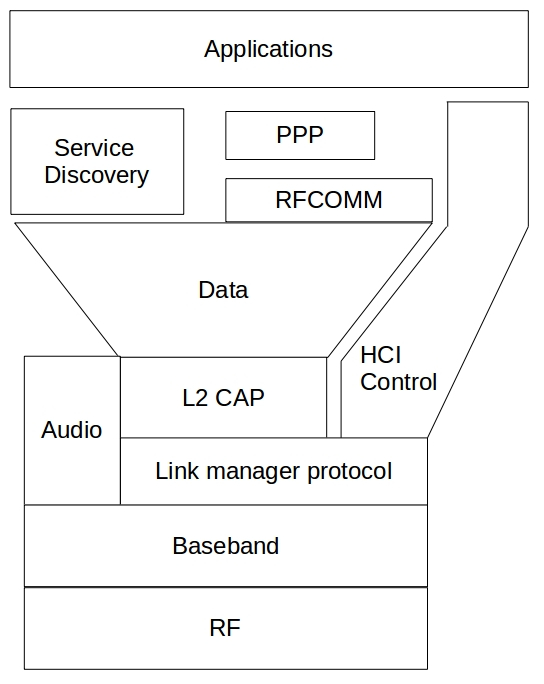
\includegraphics[scale=0.5]{bluetootharchitecturenew.jpg}  
\caption{Bluetooth Architecture}
\end{figure}
\subsubsection{Bluetooth Topology}
There can be only 2 - 7 Bluetooth devices talking to each other. This is called a piconet. Among these devices, there can be only one master device, all the rest are slave devices. A device can belong to two piconets meantime, serving as slaves in both piconet or a master in one and slave in another. This is called a bridging device. Bridging devices connect piconets together to form a scatternet:\cite{bluetooth2}
\begin{figure}[htp]
\center
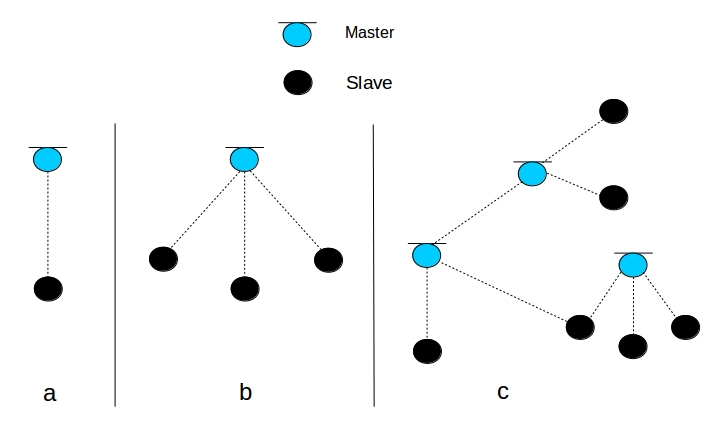
\includegraphics[scale=0.5]{topology.jpg} 
\caption{Single-slave piconet (a), multiple-slave piconet(b) and scatternet (c)}
\end{figure}
\subsubsection{RF and Baseband}
\subsubsection*{RadioFrequency}
Bluetooth operates at the unlicensed 2.5GHz Industrial-Scientific-Medical (ISM) band. There are already many types of devices using this band, such as baby monitors and garage door remote controls. To avoid interfering with these devices, Bluetooth devices sends out very weak signals (about 1 milliwatt). This limits the transmission range to 10 meters. It also uses a frequency hopping technique, hopping randomly between 79 1-MHz channels 1600 times per second (625 us time slot). Each piconet is synchronized to a specific frequency hopping pattern\cite{bluetooth2}, so that even different piconets do not interfere with each other. A piconet can either be static or dynamic (chaning when devices move in or out).
\subsubsection*{Modulation in Bluetooth}
The modulation in Bluetooth is Gaussian Frequency Shift Keying\cite{bluetooth2}(GFSK), with a BT = 0.5 and modulation index between 0.25 and 0.35.
Gaussian frequency shift keying (GFSK) is a modulation method for digital communication found in many standards such as Bluetooth, DECT and Wavenis. Digital communication amounts to translating symbols from a discrete alphabet into a signal that the transmitting side can send into a transmission medium and from which the receiving side can recover the original symbols.
\begin{figure}[h]
\center
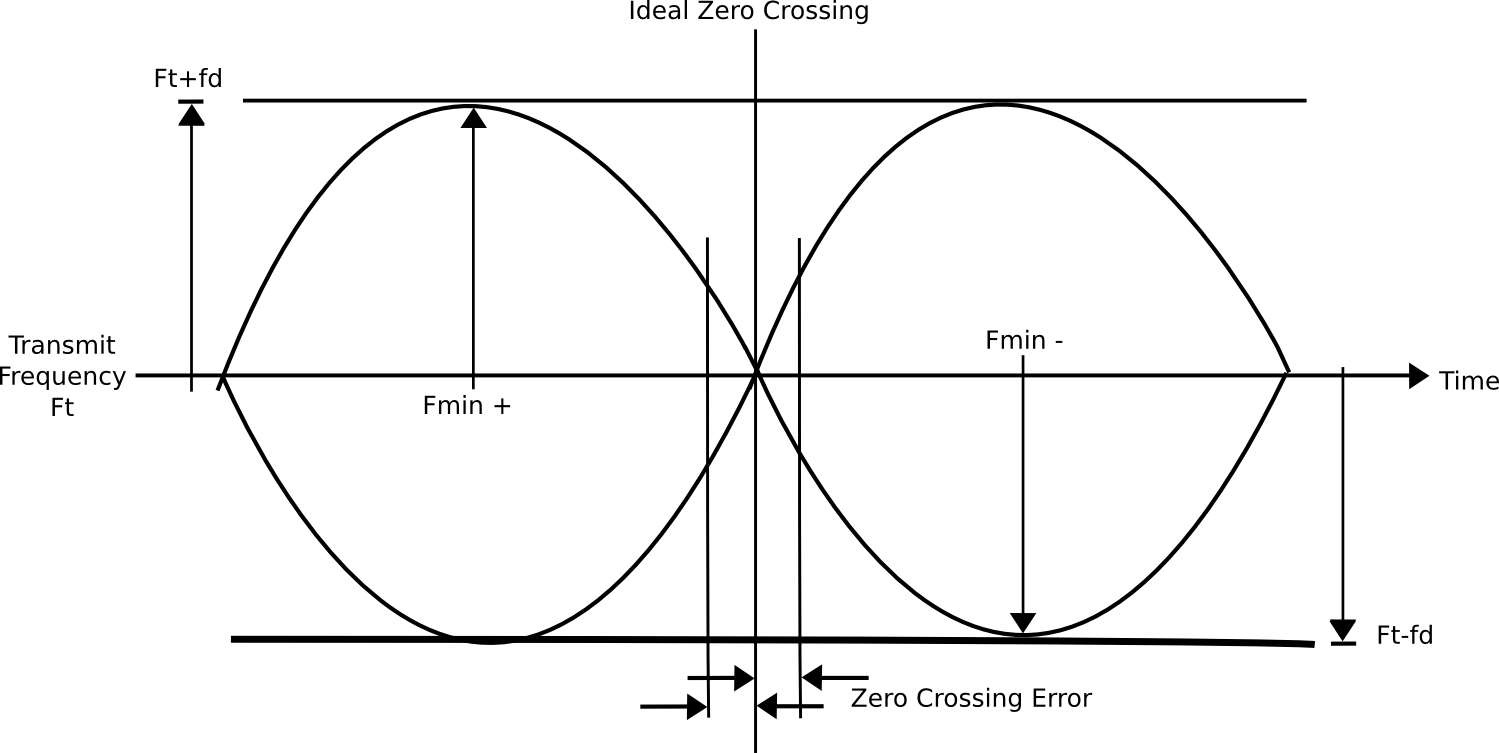
\includegraphics[scale=01]{sinewave.png}  
\caption{GFSK Modulation in Bluetooth}
\end{figure}
\subsubsection{Packet Format}
Data in piconet is encoded in packets. The general packet format is shown below:
\begin{figure}[h]
\center
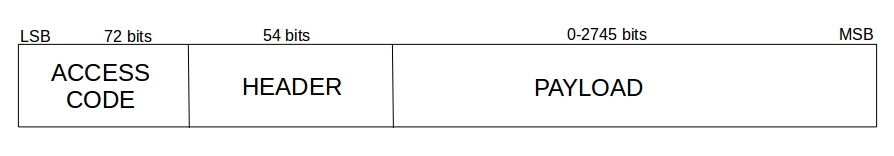
\includegraphics[scale=0.5]{first.jpg} 
\caption{General Packet Format of Bluetooth}
\end{figure}
\subsubsection*{Access Code}
Access code is used for synchronization, DC offset compensation and identification.
\subsubsection*{Header}
Header part of the packet is used by the Link Control (LC) logical channel. It has the following format:
\begin{figure}[h]
\center
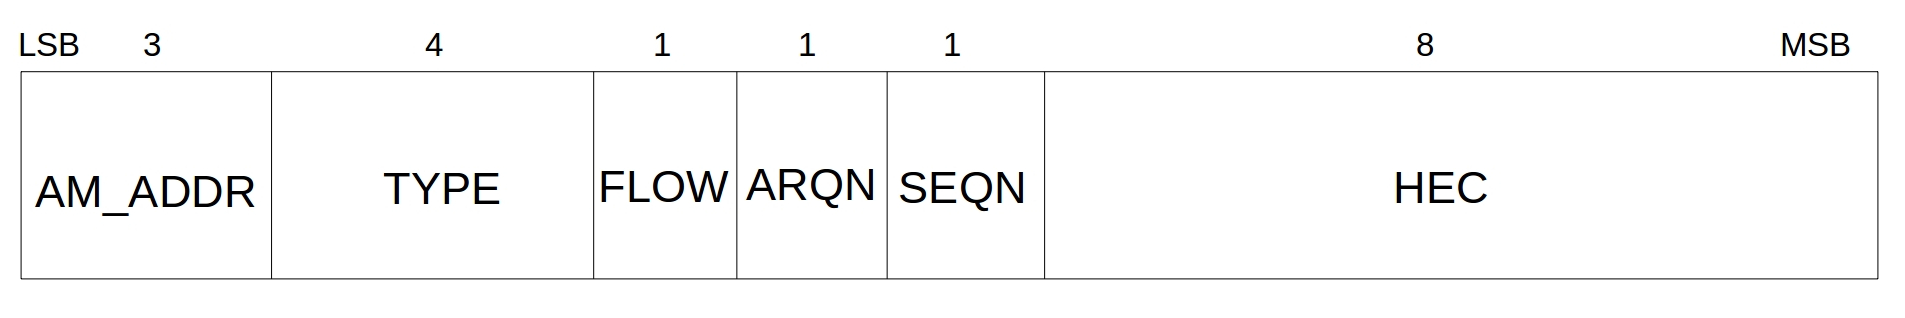
\includegraphics[scale=0.2]{second.jpg}
\caption{Header Format of Bluetooth Packet}
\end{figure}
\subsubsection*{Payload}
There can be two types of payload: voice and data. Synchronous Connection-Oriented(SCO) packets only have voice field, while Asynchronous Connectionless(ACL) packets only have data field.
\subsubsection{Physical Links}
Bluetooth protocol uses a combination of synchronous and asynchronous links. A Synchronous Connection-Oriented (SCO) link is a point-to-point link between the master and specific slave. It has symmetric 64 kbps rate, typically used for voice transmission. It uses reserved time slots, thus can be regarded as a circuit switching link. A master can support up to 3 SCO links to one or multiple slaves, while a slave can support up to three SCO links to one master or up to two SCO links to different masters. Master transmits at reserved master-to-slave time slot, and slave response in the following slave-to-master slot. SCO packets are never retransmitted.\\
Asynchronous Connectionless (ACL) links are used for data transmission, with 723.2 downstream/57.6 kbps upstream asymmetric or 433.9 kbps symmetric data rate. There can be only one ACL link between the master and all active slaves. Only the addressed slave device can response. ACL packets can be retransmitted for data integrity.
\subsection{Serial Communication}
Serial data transfer is when we transfer data one bit at a time, one right after the other. These
interfaces can operate on as little as one wire, usually never more than four.
Asynchronous mode of data transfer means that data is transferred without support from an
external clock signal. This transmission method is perfect for minimizing the required wires
and I/O pins, but it does mean we need to put some extra effort into reliably transferring and
receiving data. The asynchronous serial protocol has a number of built-in rules or
mechanisms that help ensure robust and error-free data transfers.
\subsubsection{Baud Rate}
The baud rate specifies how fast data is sent over a serial line. It’s usually expressed in units
of bits-per-second (bps) provided each signal transition represents a data transfer. If you
invert the baud rate, you can find out just how long it takes to transmit a single bit. This
value determines how long the transmitter holds a serial line high/low or at what period the
receiving device samples its line.\\
Baud rates can be just about any value within reason. The only requirement is that both
devices operate at the same rate. One of the more common baud rates, especially for simple
stuff where speed isn’t critical, is 9600 bps. Other “standard” baud are 1200, 2400, 4800,
19200, 38400, 57600, and 115200.
\subsubsection{Synchronization bits}
The synchronization bits are two or three special bits transferred with each chunk of data.
They are the start bit and the stop bit(s). There’s always only one start bit, but the number of
stop bits is configurable to either one or two. The start bit is always indicated by an idle data
line going from 1 to 0, while the stop bit(s) will transition back to the idle state by holding
the line at 1.
\subsubsection{Parity Bits}
Parity is a form of very simple, low-level error checking. It comes in two flavors: odd or
even. To produce the parity bit, all 5-9 bits of the data byte are added up, and the evenness
of the sum decides whether the bit is set or not. For example, assuming parity is set to even
and was being added to a data byte like 0b01011101, which has an odd number of 1’s (5),
the parity bit would be set to 1. Conversely, if the parity mode was set to odd, the parity bit
would be 0. Parity is optional, and not very widely used. It can be helpful for transmitting
across noisy mediums, but it’ll also slow down your data transfer a bit and requires both
sender and receiver to implement error-handling.\begin{table}[h]
\begin{center}
\begin{tabular}{ |c|c|c|c|c| } 
 \hline
 FRAME:& Start& Data &Parity& Stop\\
\hline 
SIZE (BITS):& 1& 5-9& 0-1& 1-2\\
\hline
\end{tabular}
\caption{Serial Frame}
\end{center}
\end{table}

\subsection{Microcontroller}
A microcontroller is a self-contained system with peripherals, memory and a processor that can be used as an embedded system. Most programmable microcontrollers that are used today are embedded in other consumer products or machinery including phones, peripherals, automobiles and household appliances for computer systems. Due to that, another name for a microcontroller is "embedded controller." Some embedded systems are more sophisticated, while others have minimal requirements for memory and programming length and a low software complexity. Input and output devices include solenoids, LCD displays, relays, switches and sensors for data like humidity, temperature or light level, amongst others.\\
Microcontrollers are used in automatically controlled products and devices, such as automobile engine control systems, implantable medical devices, remote controls, office machines, appliances, power tools, toys and other embedded systems. By reducing the size and cost compared to a design that uses a separate microprocessor, memory, and input/output devices, microcontrollers make it economical to digitally control even more devices and processes. Mixed signal microcontrollers are common, integrating analog components needed to control non-digital electronic systems.
\subsubsection{Embedded Design}
A microcontroller can be considered a self-contained system with a processor, memory and peripherals and can be used as an embedded system. The majority of microcontrollers in use today are embedded in other machinery, such as automobiles, telephones, appliances, and peripherals for computer systems.\\
While some embedded systems are very sophisticated, many have minimal requirements for memory and program length, with no operating system, and low software complexity. Typical input and output devices include switches, relays, solenoids, LEDs, small or custom liquid-crystal displays, radio frequency devices, and sensors for data such as temperature, humidity, light level etc. Embedded systems usually have no keyboard, screen, disks, printers, or other recognizable I/O devices of a personal computer, and may lack human interaction devices of any kind.
\subsubsection{Programming Environment}
Microcontrollers were originally programmed only in assembly language, but various high-level programming languages, such as Python and JavaScript, are now also in common use to target microcontrollers and embedded systems.These languages are either designed specially for the purpose, or versions of general purpose languages such as the C programming language. Compilers for general purpose languages will typically have some restrictions as well as enhancements to better support the unique characteristics of microcontrollers. Some microcontrollers have environments to aid developing certain types of applications.\\
Simulators are available for some microcontrollers. These allow a developer to analyze what the behavior of the microcontroller and their program should be if they were using the actual part. A simulator will show the internal processor state and also that of the outputs, as well as allowing input signals to be generated. While on the one hand most simulators will be limited from being unable to simulate much other hardware in a system, they can exercise conditions that may otherwise be hard to reproduce at will in the physical implementation, and can be the quickest way to debug and analyze problems.
\subsubsection{Types of microcontrollers}
As of 2008, there are several dozen microcontroller architectures and vendors including:
\begin{enumerate}
\item ARM core processors
\item Atmel AVR
\item Intel 8051
\item Microchip Technology PIC
\item Silicon Laboratories Pipelined 8-bit 8051 Microcontrollers and mixed-signal ARM-based 32-bit microcontrollers
\item Texas Instruments  
\end{enumerate}
\justify Many others exist, some of which are used in very narrow range of applications or are more like applications processors than microcontrollers.
\subsubsection{Input And Output}
Microcontroller systems provide multiple forms of input and output signals to allow application software to control an external "real-world" system. Discrete digital I/O provides a single bit of data (on, or off). Analog signals, representing a continuously variable range such as temperature or pressure, can also be inputs and outputs for microcontrollers.\\
One or more analog inputs, with an analog multiplexer and common analog to digital converter, are found on some microcontroller boards. Analog outputs may use a digital-to-analog converter, or on some microcontrollers may be controlled by pulse-width modulation. As for discrete inputs, external circuits may be required to scale inputs, or to provide such functions as bridge excitation or cold junction compensation.
\subsubsection{Block Diagram}
\begin{figure}[h]
\center
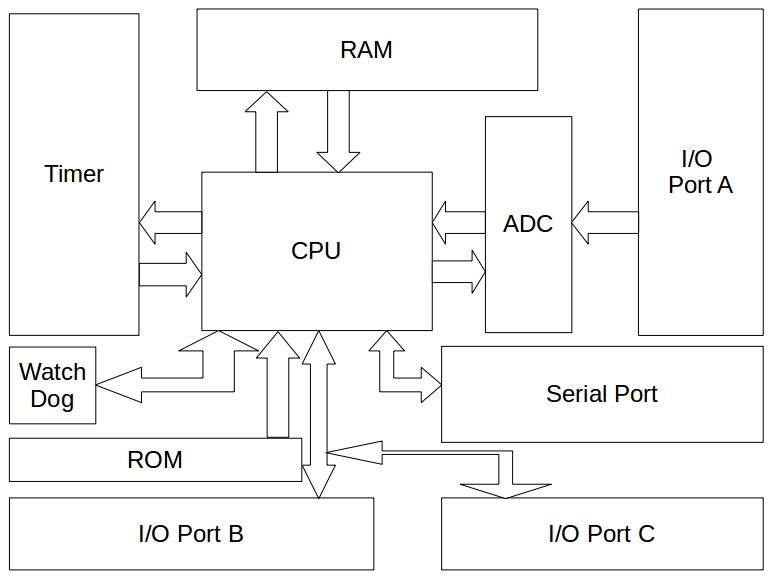
\includegraphics[scale=0.5]{microblock.jpg}  
\caption{Block Diagram of Microcontroller}
\end{figure}
\subsubsection*{Microcontroller block diagram explanation}
The explanation of the microcontroller\\cite{microcontroller} block diagram given above is as follows:
\begin{enumerate}
\item Central Processing Unit (CPU)\\
The CPU is the brain of any processing device of the microcontroller. It monitors and controls all operations that are performed on the Microcontroller units. The user has no control over the work of the CPU directly . It reads program written in ROM memory and executes them and do the expected task of that application. It performs all of the arithmetic and logic operations and controls the flow of execution of instructions.
\item Memory
Microcontroller requires a program which is a collection of instructions. This program tells microcontroller to do specific tasks. These programs require a memory on which these can be saved and read by Microcontroller to perform specific operations of a particular task. 
\begin{enumerate}
\item Random Access Memory(RAM)\\
The RAM holds the set of instructions (program). i.e. being executed by the CPU. It is a general purpose memory that can store data or programs. RAM is 'volatile', which means when the power is shut off, the contents of the memory is lost. Most personal computers have several megabytes of RAM. Most microcontrollers have some RAM built into them, but not very much. 256 bytes is a fairly common amount. Some have more, some have less. RAM is responsible for holding important data structures like 'stack'.\\
\item Read Only Memory(ROM)\\
ROM is Read Only Memory. This is typically memory that is programmed at the factory to have certain values. It cannot be changed, but it can be read as many times as wanted. ROM is typically used to store programs and data that doesn't change over time. In microcontrollers, it holds very important data and initialization about the microcontroller. It holds the monitor program and is written by the manufacturer. \\
\item Flash Memory
It is basically a Electrically Erasable Programmable Read Only Memory (EEPROM) and holds the program written by the user. The program can be erased or written here many times (specified by the manufacturer).\\
\end{enumerate}
\item Input/Output Ports\\
Normally microcontroller is used in embedded systems to control the operation of machines in the microcontroller. Therefore, to connect it to other machines, devices or peripherals we require I/O interfacing ports in the microcontroller interface. For example, microcontroller 8051 has 4 input, output ports to connect it to the other peripherals. Each port in a microcontroller is made up of n-pins (mostly 8 pins). Each pin can be configured as either input or output pin. If a pin is input pin, it accepts data from the device it is connected to. Similarly, if a pin is a output pin, it sends the data to the device it is connected to.
\item Analog to Digital Converter (ADC)\\
Most of the real world signals are analog in nature. But, a microcontroller is a digital device. Hence, it cannot process analog signals. This is why all microcontrollers have a built-in analog-to-digital converter. ADC digitizes an analog signal and gives it to the microcontroller for further processing. The conversion involves quantization of the input, so it necessarily introduces a small amount of error. Furthermore, instead of continuously performing the conversion, an ADC does the conversion periodically, sampling the input. The result is a sequence of digital values that have been converted from a continuous-time and continuous-amplitude analog signal to a discrete-time and discrete-amplitude digital signal.
\item Timers/Counters\\
Every microcontroller comes with one or more (sometimes many more) built-in timer/counters, and these are extremely useful. The term timer/counter itself reflects the fact that the underlying counter hardware can usually be configured to count either regular clock pulses (making it a timer) or irregular event pulses (making it a counter). The timer and counter functions in the microcontroller count in sync with the microcontroller clock. However, the counter only counts up to to either 256 (8 bit counter) or 65535 (16 bit counter). The microcontroller offers a quite useful feature called prescaling. Prescaling is a simplistic way for the counter to skip a certain number of clock ticks.\\
\item Interrupts\\
As its name suggests, Interrupt is a subroutine call that interrupts of the microcontrollers main operations or work and causes it to execute any other program, which is more important at the time of operation. The feature of Interrupt is very useful as it helps in case of emergency operations. An Interrupts gives us a mechanism to put on hold the ongoing operations, execute a subroutine and then again resumes to another type of operations.\\ 
\item Watchdog \\
A watchdog timer (WDT) is an embedded timing device that automatically prompts corrective action upon system malfunction detection. If software hangs or is lost, a WDT resets the system microcontroller via a 16-bit counter. A WDT is also known as a computer operating properly (COP) timer.\\
A WDT enables embedded system self-reliance in two ways:
\begin{enumerate}
\item Detects system glitches or errors, including programming errors, software hangs, code crashes or power surges. 
\item Resets operating systems and resumes normal program activity via the reset signal embedded in a CPU or specialized microcontroller chip. This reset process is also known as feeding the watchdog, kicking the dog, waking the watchdog or petting the dog. 
\end{enumerate}
\end{enumerate}
\subsubsection{Arduino UNO}
Arduino/Genuino Uno is a microcontroller board based on the ATmega328P. It has 14 digital input/output pins (of which 6 can be used as PWM outputs), 6 analog inputs, a 16 MHz quartz crystal, a USB connection, a power jack, an In-Circuit Serial Programming(ICSP) header and a reset button. It contains everything needed to support the microcontroller; simply connectable to a computer with a USB cable or can be powered with a AC-to-DC adapter or battery.Some of the important specification\cite{arduino} for Arduino UNO are: 
\begin{table}
\center
\begin{tabular}{ |p{5cm}|p{7cm}| }
\hline
\multicolumn{2}{|c|}{Specifications} \\
\hline
MicroController& ATMega328P \\
\hline
Operating Voltage& 5V\\
\hline
Input Voltage (recommended) & 7-12 V\\
\hline
Input Voltage (limit) &6-20V\\
\hline
Digital I/O pins &14(of which 6 provide PWM output) \\
\hline
PWM Digital I/O pins&6\\
\hline
Analag Input Pins & 6 \\
\hline
DC Current per I/O Pin	& 20 mA\\
\hline
DC Current for 3.3V Pin	& 50 mA\\
\hline
Flash Memory	& 32 KB (ATmega328P)
of which 0.5 KB used by bootloader\\
\hline
SRAM	& 2 KB (ATmega328P)\\
\hline
EEPROM	& 1 KB (ATmega328P)\\
\hline
Clock Speed	& 16 MHz\\
\hline
Length	& 68.6 mm\\
\hline
Width	& 53.4 mm\\
\hline
Weight	& 25 g\\
\hline
\end{tabular}
\caption{Arduino UNO Specifications}
\end{table}



\subsection{ FC -51: InfraRed Sensor}
Infrared technology addresses a wide variety of wireless applications. The main areas are sensing and remote controls. In the electromagnetic spectrum, the infrared portion is divided into three regions: near infrared region, mid infrared region and far infrared region.\\
The frequency range of infrared is higher than microwave and lesser than visible light.\\
For optical sensing and optical communication, photo optics technologies are used in the near infrared region as the light is less complex than RF when implemented as a source of signal. Optical wireless communication is done with IR data transmission for short range applications.\\
An infrared sensor emits and/or detects infrared radiation to sense its surroundings.\\
The working of any Infrared sensor is governed by three laws: Planck’s Radiation law, Stephen – Boltzmann law and Wien’s Displacement law.\\
Planck’s law states that “every object emits radiation at a temperature not equal to 00K”. Stephen – Boltzmann law states that “at all wavelengths, the total energy emitted by a black body is proportional to the fourth power of the absolute temperature”. According to Wien’s Displacement law, “the radiation curve of a black body for different temperatures will reach its peak at a wavelength inversely proportional to the temperature”.\\
The basic concept of an Infrared Sensor which is used as Obstacle detector is to transmit an infrared signal, this infrared signal bounces from the surface of an object and the signal is received at the infrared receiver.\\
There are five basic elements used in a typical infrared detection system: an infrared source, a transmission medium, optical component, infrared detectors or receivers and signal processing. Infrared lasers and Infrared LED’s of specific wavelength can be used as infrared sources. The three main types of media used for infrared transmission are vacuum, atmosphere and optical fibers. Infrared receivers can be photodiodes, phototransistors etc. some important specifications of infrared receivers are photosensitivity, detectivity and noise equivalent power. Signal processing is done by amplifiers as the output of infrared detector is very small.\\
FC-51 is an active sensor and its constituent and working principle are as explained below: \\
Active infrared sensors consist of two elements: infrared source and infrared detector. Infrared sources include an LED or infrared laser diode. Infrared detectors include photodiodes or phototransistors. The energy emitted by the infrared source is reflected by an object and falls on the infrared detector.
\subsubsection{InfraRed Transmitter}
Infrared Transmitter is a light emitting diode (LED) which emits infrared radiations. Hence, they are called IR LED’s. Even though an IR LED looks like a normal LED, the radiation emitted by it is invisible to the human eye.\\
The picture of a typical Infrared LED is shown below.
\begin{figure}[h]
\center
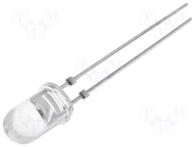
\includegraphics[scale=.5]{IR2.PNG} 
\caption{InfraRed LED }
\end{figure}
\justify There are different types of infrared transmitters depending on their wavelengths, output power and response time.\\
When operated at a supply of 5V, the IR transmitter consumes about 3 to 5 mA of current. \\
IR transmitters can be found in several applications. Some applications require infrared heat and the best infrared source is infrared transmitter. When infrared emitters are used with Quartz, solar cells can be made.
\subsubsection{InfraRed Receiver}
Infrared receivers are also called as infrared sensors as they detect the radiation from an IR transmitter. IR receivers come in the form of photodiodes and phototransistors. Infrared Photodiodes are different from normal photo diodes as they detect only infrared radiation. The picture of a typical IR receiver or a photodiode is shown below.
\begin{figure}[h]
\center
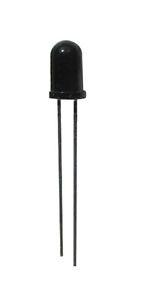
\includegraphics[scale=0.5]{IRR.jpg} 
\caption{IR Receiver }
\end{figure}
\justify Different types of IR receivers exist based on the wavelength, voltage, package, etc. When used in an infrared transmitter – receiver combination, the wavelength of the receiver should match with that of the transmitter.
\subsubsection{Working Principle }
\begin{figure}[h]
\center
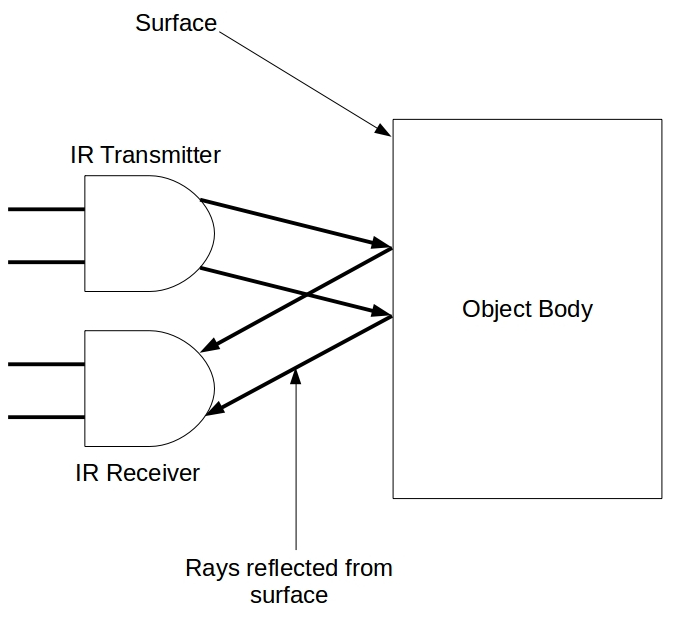
\includegraphics[scale=0.5]{IRpair.jpg} 
\caption{Working Schematic of IR Sensor }
\end{figure}
\justify The principle of an IR sensor working as an Object Detection Sensor can be explained using the following above figure. An IR sensor consists of an IR LED and an IR Photodiode; together they are called as Photo – Coupler or Opto – Coupler.
When the IR transmitter emits radiation, it reaches the object and some of the radiation reflects back to the IR receiver. Based on the intensity of the reception by the IR receiver, the output of the sensor is defined.
\subsubsection{Obstacle Sensing Circuit or IR Sensor Circuit}
A typical IR sensing circuit is shown below.\\
\begin{figure}[h]
\newpage
\center
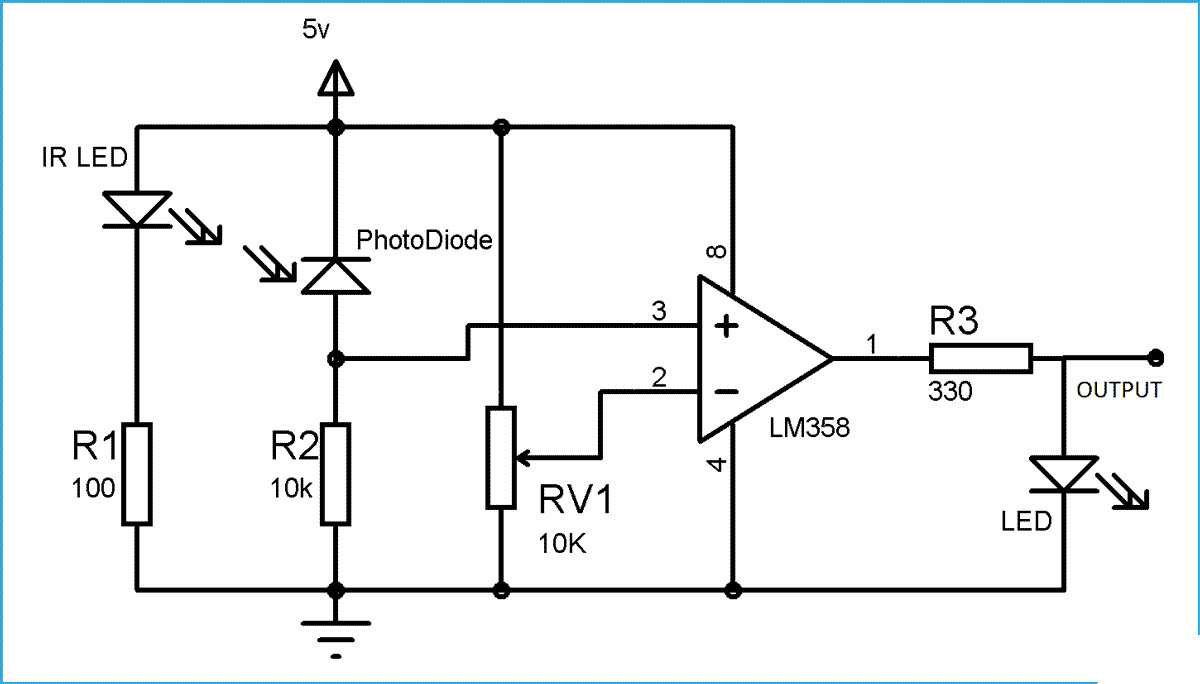
\includegraphics[scale=0.4]{IRsensorcircuit.jpg} 
\caption{IR Sensing circuit Schematic}
\end{figure}
It consists of an IR LED, a photodiode, a potentiometer, an IC Operational amplifier and an LED.\\
IR LED emits infrared light. The Photodiode detects the infrared light. An IC Op – Amp is used as a voltage comparator. The potentiometer is used to calibrate the output of the sensor according to the requirement.\\
When the light emitted by the IR LED is incident on the photodiode after hitting an object, the resistance of the photodiode falls down from a huge value. One of the input of the op – amp is at threshold value set by the potentiometer. The other input to the op-amp is from the photodiode’s series resistor. When the incident radiation is more on the photodiode, the voltage drop across the series resistor will be high. In the IC, both the threshold voltage and the voltage across the series resistor are compared. If the voltage across the resistor series to photodiode is greater than that of the threshold voltage, the output of the IC Op – Amp is high. As the output of the IC is connected to an LED, it lightens up. The threshold voltage can be adjusted by adjusting the potentiometer depending on the environmental conditions.\\
The positioning of the IR LED and the IR Receiver is an important factor. When the IR LED is held directly in front of the IR receiver, this setup is called Direct Incidence. In this case, almost the entire radiation from the IR LED will fall on the IR receiver. Hence there is a line of sight communication between the infrared transmitter and the receiver. If an object falls in this line, it obstructs the radiation from reaching the receiver either by reflecting the radiation or absorbing the radiation.\\
The Infra-Red Sensor module used in the project is the FC-51 Sensor Module\cite{fc51}. It is a Infrared Obstacle Avoidance Proximity Sensor.\\ 
Infrared Obstacle Avoidance Proximity Sensors Module has builtin IR transmitter and IR receiver that sends out IR energy and looks for reflected IR energy to detect presence of any obstacle in front of the sensor module. The module has on board potentiometer that lets user adjust detection range. The sensor has very good and stable response even in ambient light or in complete darkness.\\
The sensor module can be interfaced with Arduino, Raspberry Pi or any microcontroller having IO voltage level of 3.3V to 5V.
\subsection*{Applications}
\begin{enumerate}
\item Obstacle avoidance in robots 
\item Production counting on assembly lines 
\item Presence detection 
\item Security systems 
\end{enumerate}
\subsection*{Features}
\begin{enumerate}
\item LM393 Comparator based detetction circuit is very stable and accurate 
\item On board potentiometer sets obstacle detection range 
\item On board Power LED indicator 
\item On board Obsatcle Detection LED indicator 
\item 3.0MM mounting hole for easy mounting the sensor. 
\item Male header for easy connection 
\item Good Accuracy: By use of Infra-red LED transmitter the module performs well in Ambient light
\end{enumerate}
 \subsection*{Technical Specifications}
\begin{enumerate}
\item  Model Number: FC-51 
\item Detection angle: 35 degree
\item Operating Voltage: 3.0V – 6.0V 
\item Detection range: 2cm – 30cm (Adjustable using potentiometer) 
\item  Overall Dimension: 4.5cm (L) x 1.4 cm (W), 0.7cm (H) 
\item Active output level: Outputs Low logic level when obstacle is detected 
\item In-active output level: Outputs High logic level when obstacle is not detected 
\item Current Consumption: 
\begin{enumerate}
\item at 3.3V : ~23 mA 
	\item at 5.0V: ~43 mA 
\end{enumerate}	
\end{enumerate}

\subsection{MQ-2: SMOKE SENSOR}
In current technology scenario, monitoring of gases produced is very important. From home appliances such as air conditioners to electric chimneys and safety systems at industries monitoring of gases is very crucial. Gas sensors are very important part of such systems.  Small like a nose, gas sensors spontaneously react to the gas present, thus keeping the system updated about any alterations that occur in the concentration of molecules at gaseous state.\\
Gas sensors are available in wide specifications depending on the sensitivity levels, type of gas to be sensed, physical dimensions and numerous other factors. This Insight covers a methane gas sensor that can sense gases such as ammonia which might get produced from methane. When a gas interacts with this sensor, it is first ionized into its constituents and is then adsorbed by the sensing element. This adsorption creates a potential difference on the element which is conveyed to the processor unit through output pins in form of current. \\
The gas sensor module consists of a steel exoskeleton under which a sensing element is housed. This sensing element is subjected to current through connecting leads. This current is known as heating current through it, the gases coming close to the sensing element get ionized and are absorbed by the sensing element. This changes the resistance of the sensing element which alters the value of the current going out of it.\\
A standard gas sensor module consists of a steel mesh, copper clamping ring and connecting leads. The top part is a stainless steel mesh which takes care of the following:
\begin{enumerate}
\item Filtering out the suspended particles so that only gaseous elements are able to pass to insides of the sensor.  
\item Protecting the insides of the sensor.
\item Exhibits an anti explosion network that keeps the sensor module intact at high temperatures and gas pressures.
\end{enumerate}
\justify The connecting leads of the sensor are thick so that sensor can be connected firmly to the circuit and sufficient amount of heat gets conducted to the inside part. They are casted from copper and have tin plating over them. Four of the six leads (A, B, C, D) are for signal fetching while two (1,2) are used to provide sufficient heat to the sensing element.
\subsubsection{Structure of MQ-2 Gas Sensor}
\begin{figure}[h]
\center
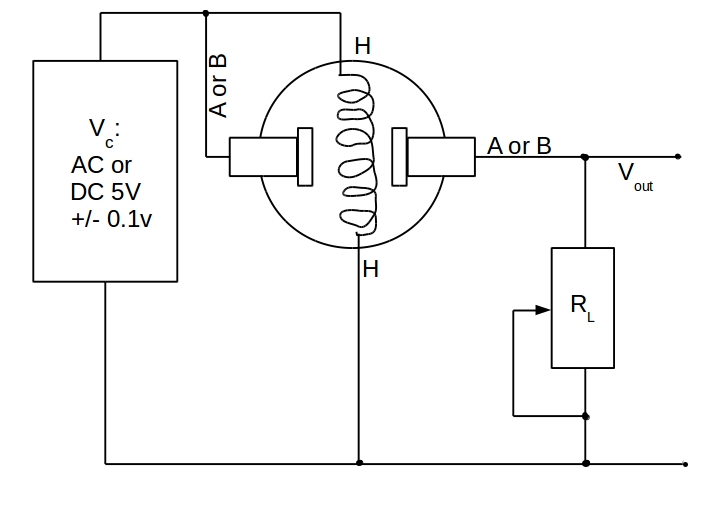
\includegraphics[scale=0.5]{smoke_new.jpg} 
\caption{Structure $\&$ configuration}
\end{figure}
\justify MQ-2 gas sensor has high sensitivity to LPG, Propane and Hydrogen, also could be used to Methane and other combustible steam, it is low cost and suitable for various applications.\\
Using high-quality dual-panel\cite{mq2datasheet} design, with a power indicator and TTL signal output instructions; With a the DO switch signal (TTL) output, and AO analog signal output; TTL output valid signal is low level; (When the low level output signal lights, it can be connected directly to the microcontroller or relay module).\\
TTL output signal can be connected directly to a microcontroller IO port or connect to the relay module, potentiometer is used to adjust the output level transition threshold.
\subsection*{Applications}
They are used in gas leakage detecting equipment in family and industry, are suitable for detecting
of LPG, i-butane, propane, methane ,alcohol, Hydrogen, smoke.
\subsection*{Features}
\begin{enumerate}
\item Wide detecting scope 
\item Fast response and High sensitivity
\item Stable and long life 
\item Simple drive circuit
\item Analog and Digital Outputs
\item Trigger Level configuration Potentiometer 
\end{enumerate}
\subsection*{Technical Specificaations}
\begin{enumerate}
\item Model: FC-22-A
\item Operating voltage: DC 5V
\item Analog Output (AO): 0~5V analog output voltage
\item Digital Outout (DO): 0V or 5V output
\item Configuration: Through Potentiometer (adjusts the output level transition)
\item Preheat Duration: 20s
\end{enumerate}

\newpage
%==============================================
\section{METHODOLOGY}
\subsection{System Architecture}
\begin{figure}[h]
\center
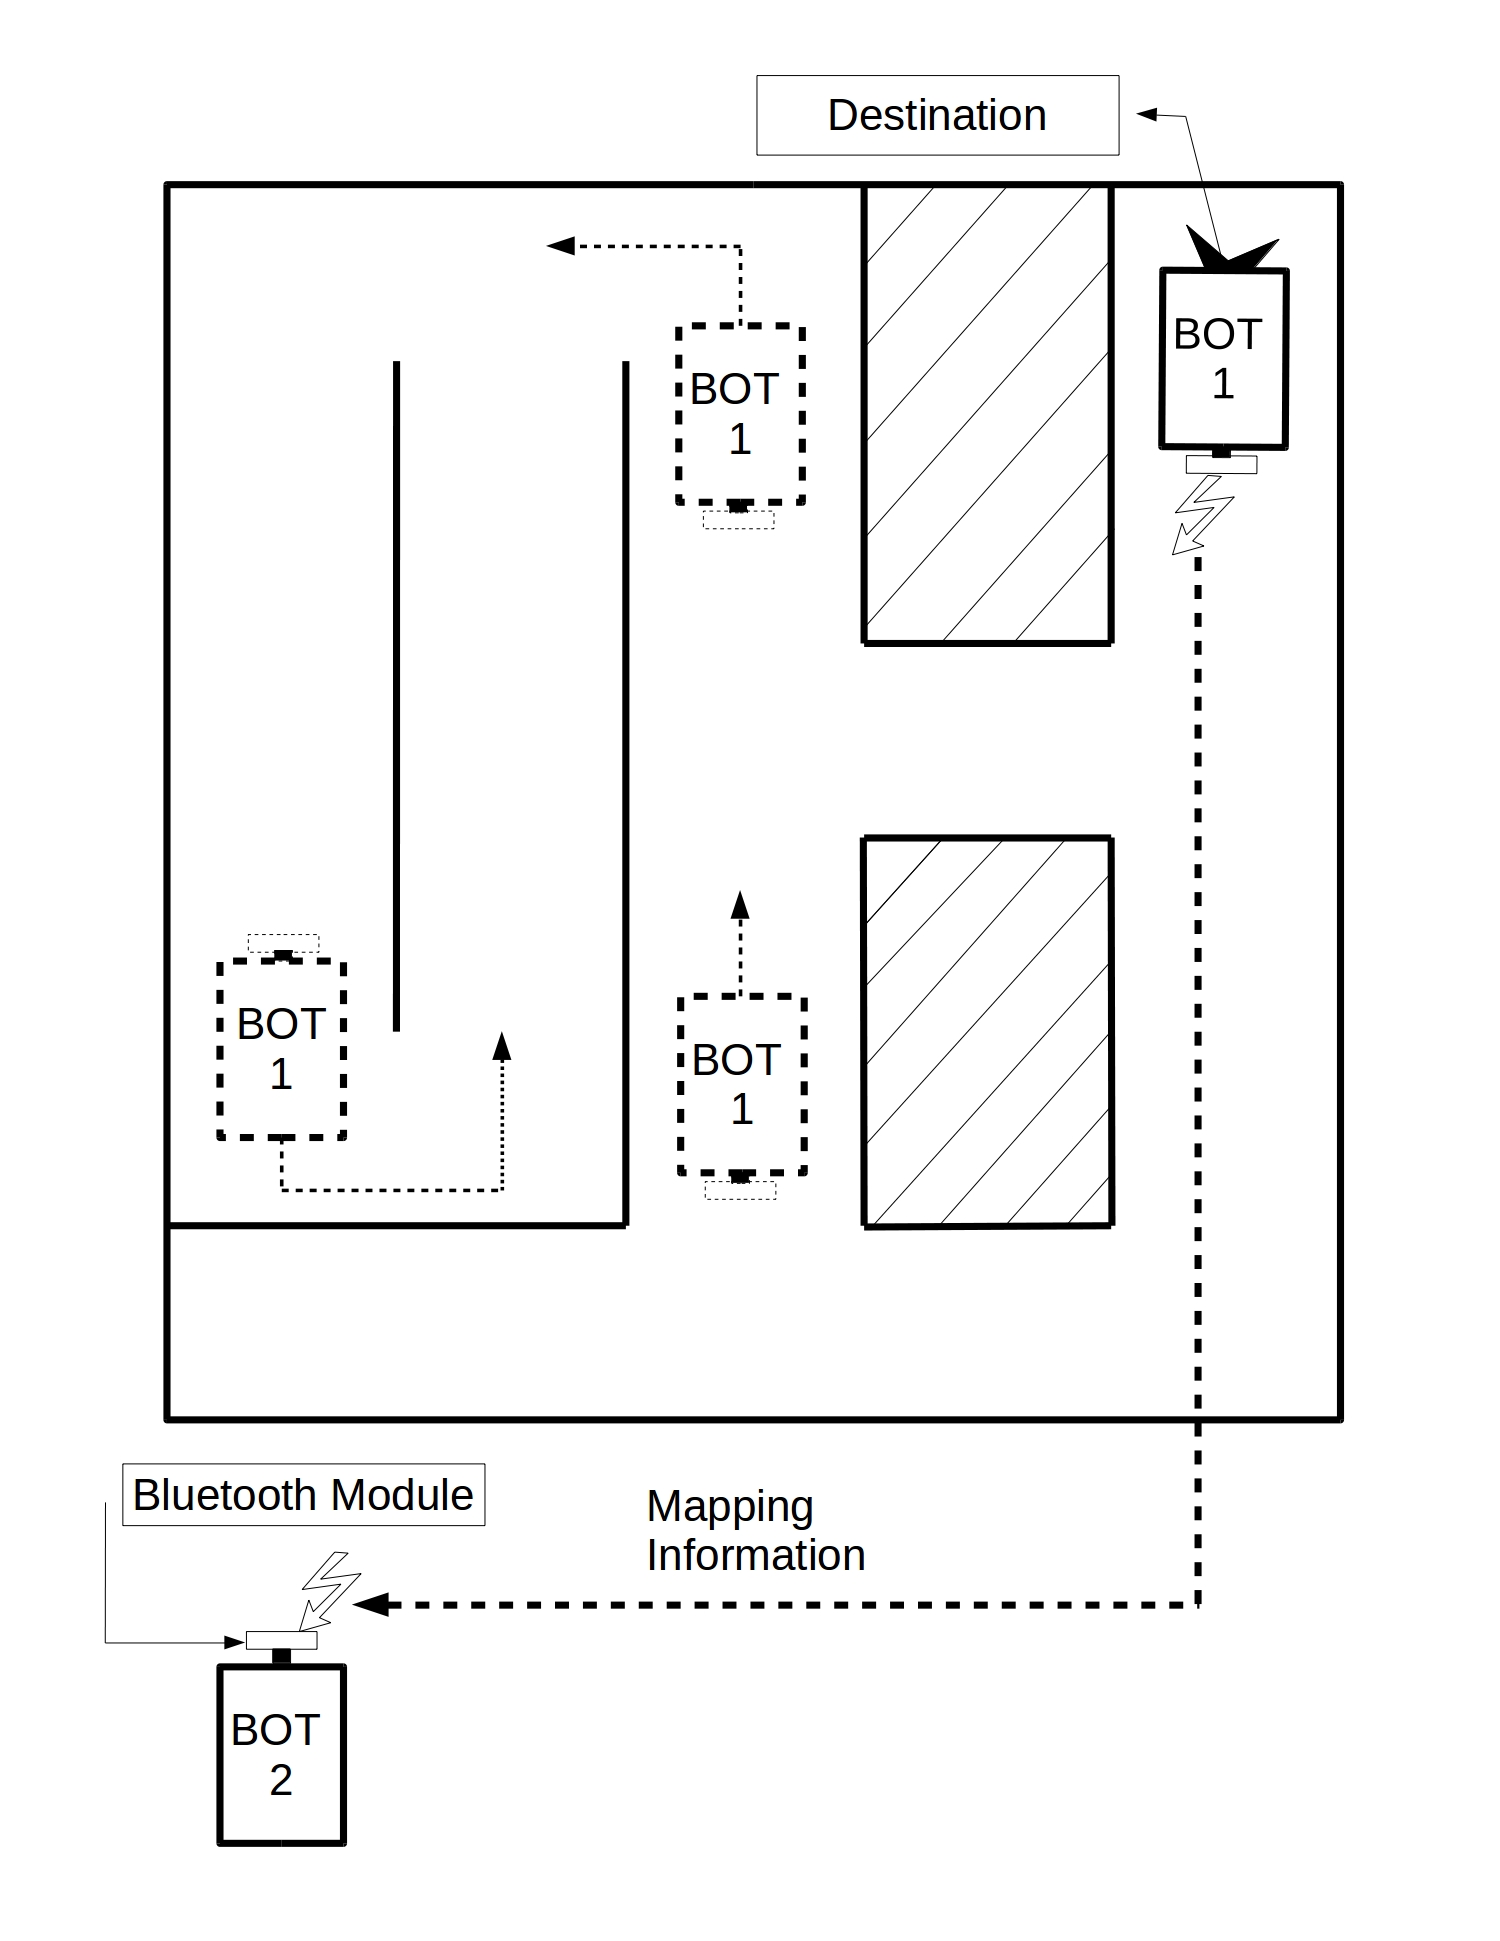
\includegraphics[scale=0.25]{systemblockdiagram_new.jpg} 
\caption{System Architecture}
\end{figure}
\justify The system contains two robotic agents. The two agents don't share the maze at the same time. First, one agent traverses the whole maze and relays the information it gathered, to the second agent via Bluetooth. The second agent will use the information provided by the first agent to solve the maze through the most optimal path. \\
The complete functional block diagram of the system is as shown below:
\begin{figure}[h]
\center
  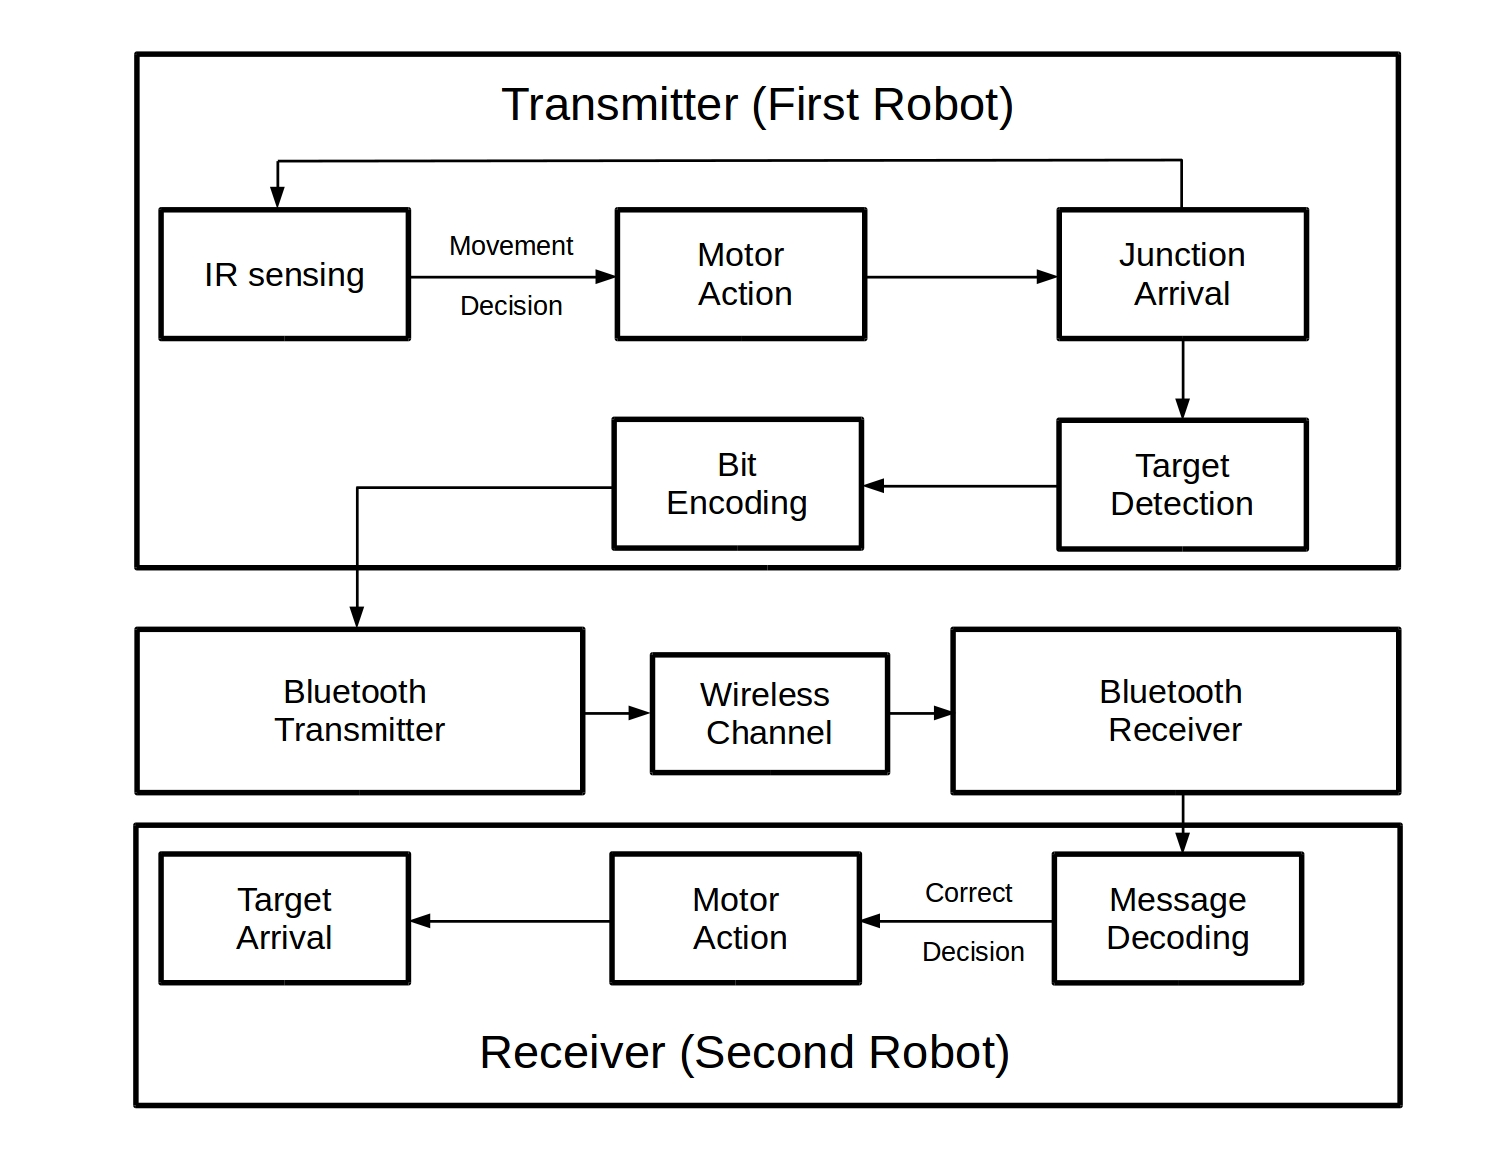
\includegraphics[scale=0.25]{funtionblock_new.jpg} 
\caption{The functional block Diagram for the system}
\end{figure}
\justify The maze solving is carried out in several steps as shown by the functional block diagram. First, the IR  sensors in the first robot detect the walls based upon which the movement decision is made. The motor action takes place according to the movement decision which is determined by the program in the microcontroller. As the motor action takes the drives the robot either left, straight or right, it reaches a junction at some point. Until the target is detected by the smoke sensor, the above process continues.\\
When the target has been detected, the shortest path information is encoded and sent to the second robot through bluetooth. Air acts as the channnel for transmission of information where noise is added during transmission. At the receiving side i.e. the second robot the information is decoded into direction information at the junction. These decisions are carried out only at the junctions which is again detected through IR sensing. The difference between the two robots is that, the second one takes the correct direction when it encounters a junction and through respective motor action, it reaches the target. 

\subsection{Maze Structure}
\begin{figure}[h]
\center
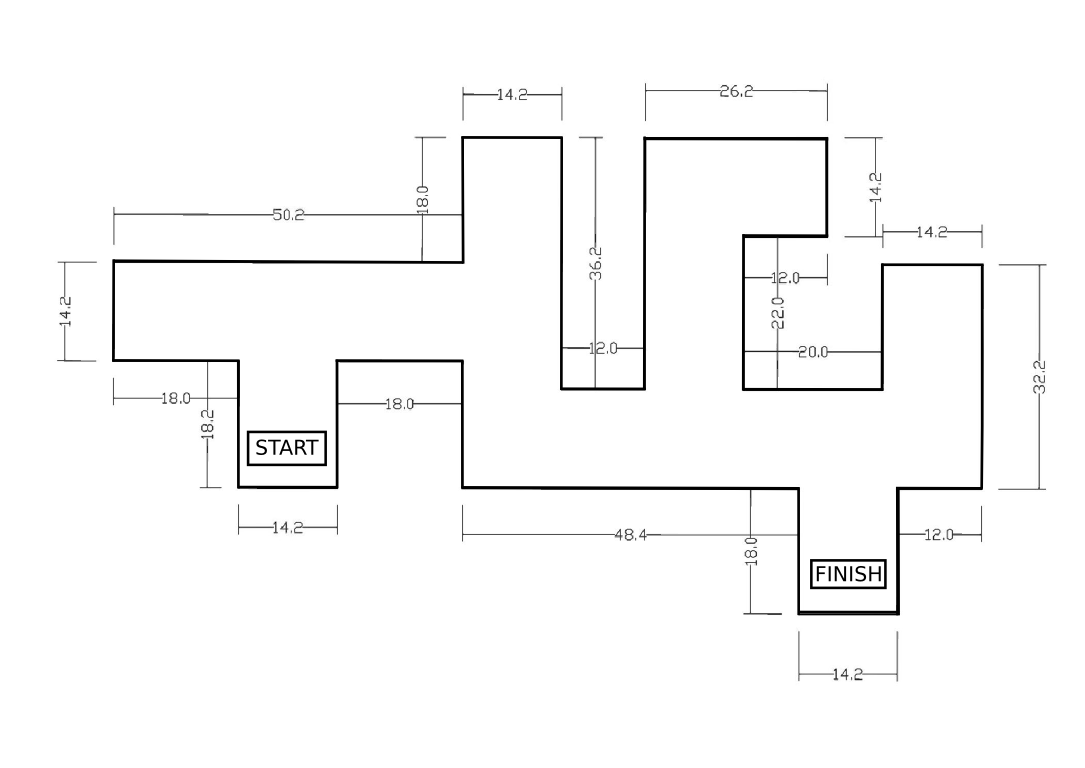
\includegraphics[scale=0.25]{top_view_lowres.png}    
\caption{Top View of the maze}
\end{figure}
\justify The figure above shows the detailed description of the maze used in the project. The dimensions of the maze walls are described in the figure as well. All the walls in the maze have a uniform height of 6 inches. The width of the path that the robot drives in is 14.2 inches wide. The appropriate distance between the two walls for the robot to drive through was selected by a trial and error process where the robot was made to run in paths of various widths. Suitable width was required for the robot to make the U-turn properly without making contact with the walls. Similarly, the sensing distance for the right and left sensors was kept in mind while determining the width.\\
For the purpose of implementing “Left Wall Following” algorithm, a simply connected maze was designed. This means that all the walls of the maze are connected together. 
The start point of the maze is selected as shown in the figure. Similarly, the target is placed along one of the maze boundaries. The dimensions of the maze is summarized below:
\begin{itemize}
\item Wall height – 6 inches
\item Width between two walls – 14.2 inches
\item Total length along the longest side – 124.8 inches 
\item Total width – 68.4 inches
\end{itemize}
\justify The maze is designed in such a way that when the first robot traverses through it, it goes through multiple U-turns and commits several mistakes before finally reaching the target. This way, when the shortest path to the target is decoded, the second robot does not go through any U-turn and follows a simple path to the target.\\
The maze structure was designed using AutoCAD and its 3-dimensional model is shown below:
\begin{figure}[h]
\center
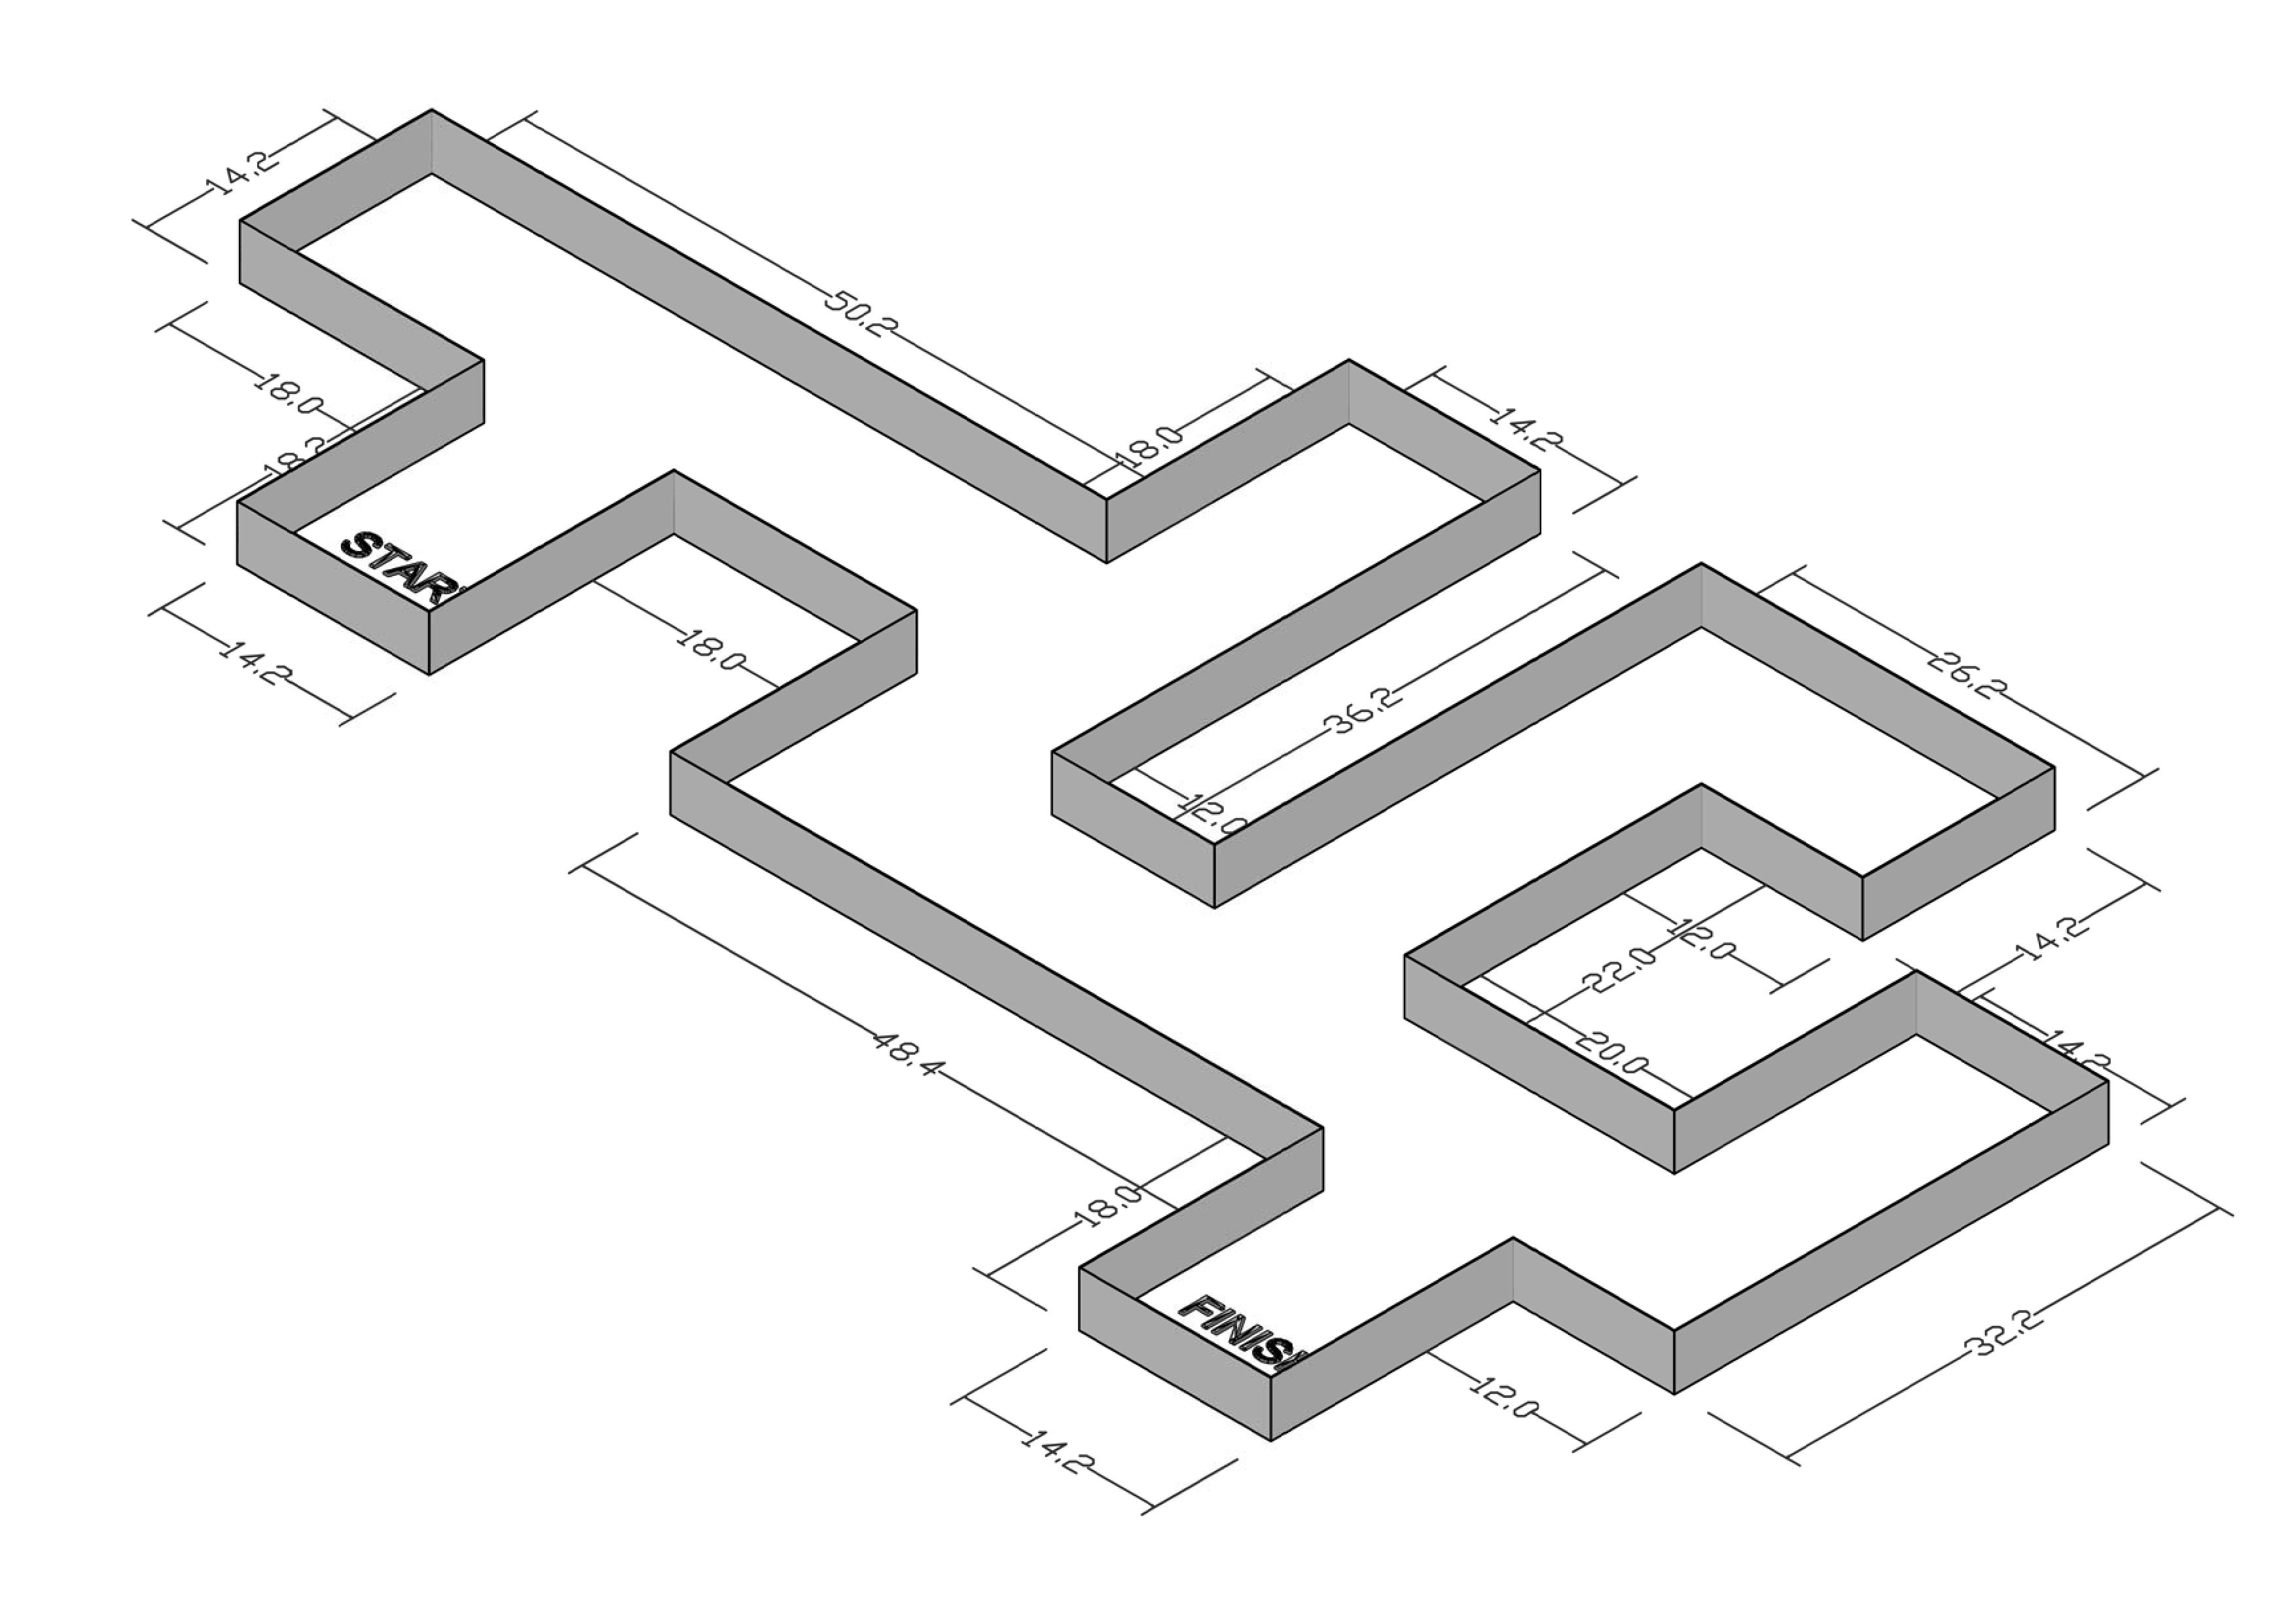
\includegraphics[scale=0.6]{maze2.jpg}   
\caption{Angular View of the maze}
\end{figure}
\subsection{Configuration of Robots}
The robots used as the agents of the swarm are two differentially driven robotic vehicles as shown in the figure. The rear wheel are driven by the PWM signal generated at the processor, which in our case is the Arduino.\\
Both the agents have two rear wheels which are rotated using a DC motor each mounted on the axle of the wheel. The degree of freedom for each of the rear wheel is two i.e. it can be rotated or moved in two direction viz. forward and backward. The rear wheels are composed of plastic tire surrounding the circular frame as shown in the figure.
\begin{figure}[h]
\center
\includegraphics[scale=0.25]{DSC_0023.JPG}    
\caption{The wheel of the robot}
\end{figure}
\justify At the front end of the robots is a caster ball wheel. In this type of wheel, a spherical metal ball is held within a vertical holder. The caster ball wheel helps balancing the robot. The use of the caster ball wheel can be justified as our project is not concerned with the motion in the rough terrain.
\newpage
\begin{figure}[h]
\center
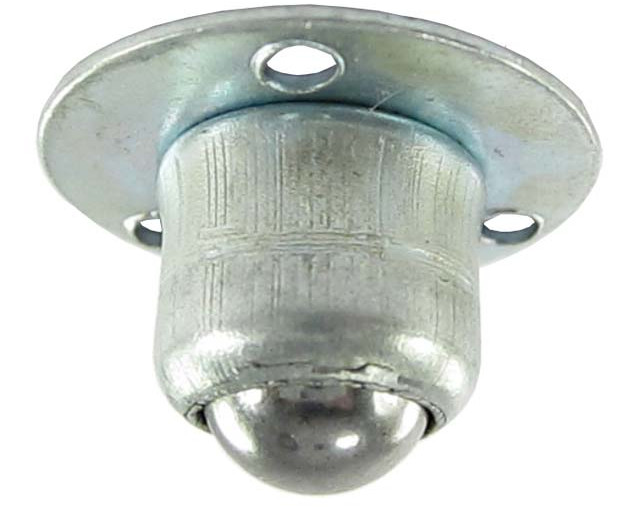
\includegraphics[scale=0.5]{caster.JPG}    
\caption{Caster wheel used in the robot}
\end{figure}
\justify The physical dimensions of the different parts of the robot are tabulated below:
\begin{table}[h]
\begin{center}
\begin{tabular}{|c|c|}
\hline
Length of robot	&8.27”\\
\hline 
Width of robot	&3.93” at the shorter side / 5.9” at the longer side\\
\hline 
Diameter of rear wheels	& 2.52”\\
\hline 
Diameter of front caster wheel&	11mm\\
\hline
\end{tabular}
\end{center}
\caption{The physical dimension of the robot}
\end{table}
\justify The electrical properties of the robot is described in the table below:
\newpage
\begin{table}
\begin{center}
\begin{tabular}{|c|c|}
\hline
Total source voltage &7.4V\\
\hline
Voltage to Arduino &5V\\
\hline 
Voltage to IR sensor& 5V\\
\hline 
Voltage to Smoke sensor& 5V\\
\hline 
Voltage to Bluetooth &3.3V\\
\hline 
Current to each IR sensor& 43mA\\
\hline 
Total current to all IR sensors& 43*3mA = 129mA\\
\hline 
Current through Smoke sensor &800mA\\
\hline
\end{tabular}
\end{center}
\caption{The electrical properties of the robot}
\end{table}
\subsubsection{First Robot}
Aside from the descriptions for the robot given above, the first robot consists of several sensor modules. It has 3 IR sensors attached at the front, left and right sides of the body. The smoke sensor is also attached at the front end besides the IR sensor. Similarly, the bluetooth module HC-05 is attached at the rear end of the robot . With the motor controller attached at the centre of the body and the arduino behind it, the battery had to be attached at the back side of the robot.\\
The entire body is made up of acrylic. Small holes are drilled at various locations in the body which allows the sensors and modules to be attached firmly. 
\newpage
\begin{figure}[h]
\center
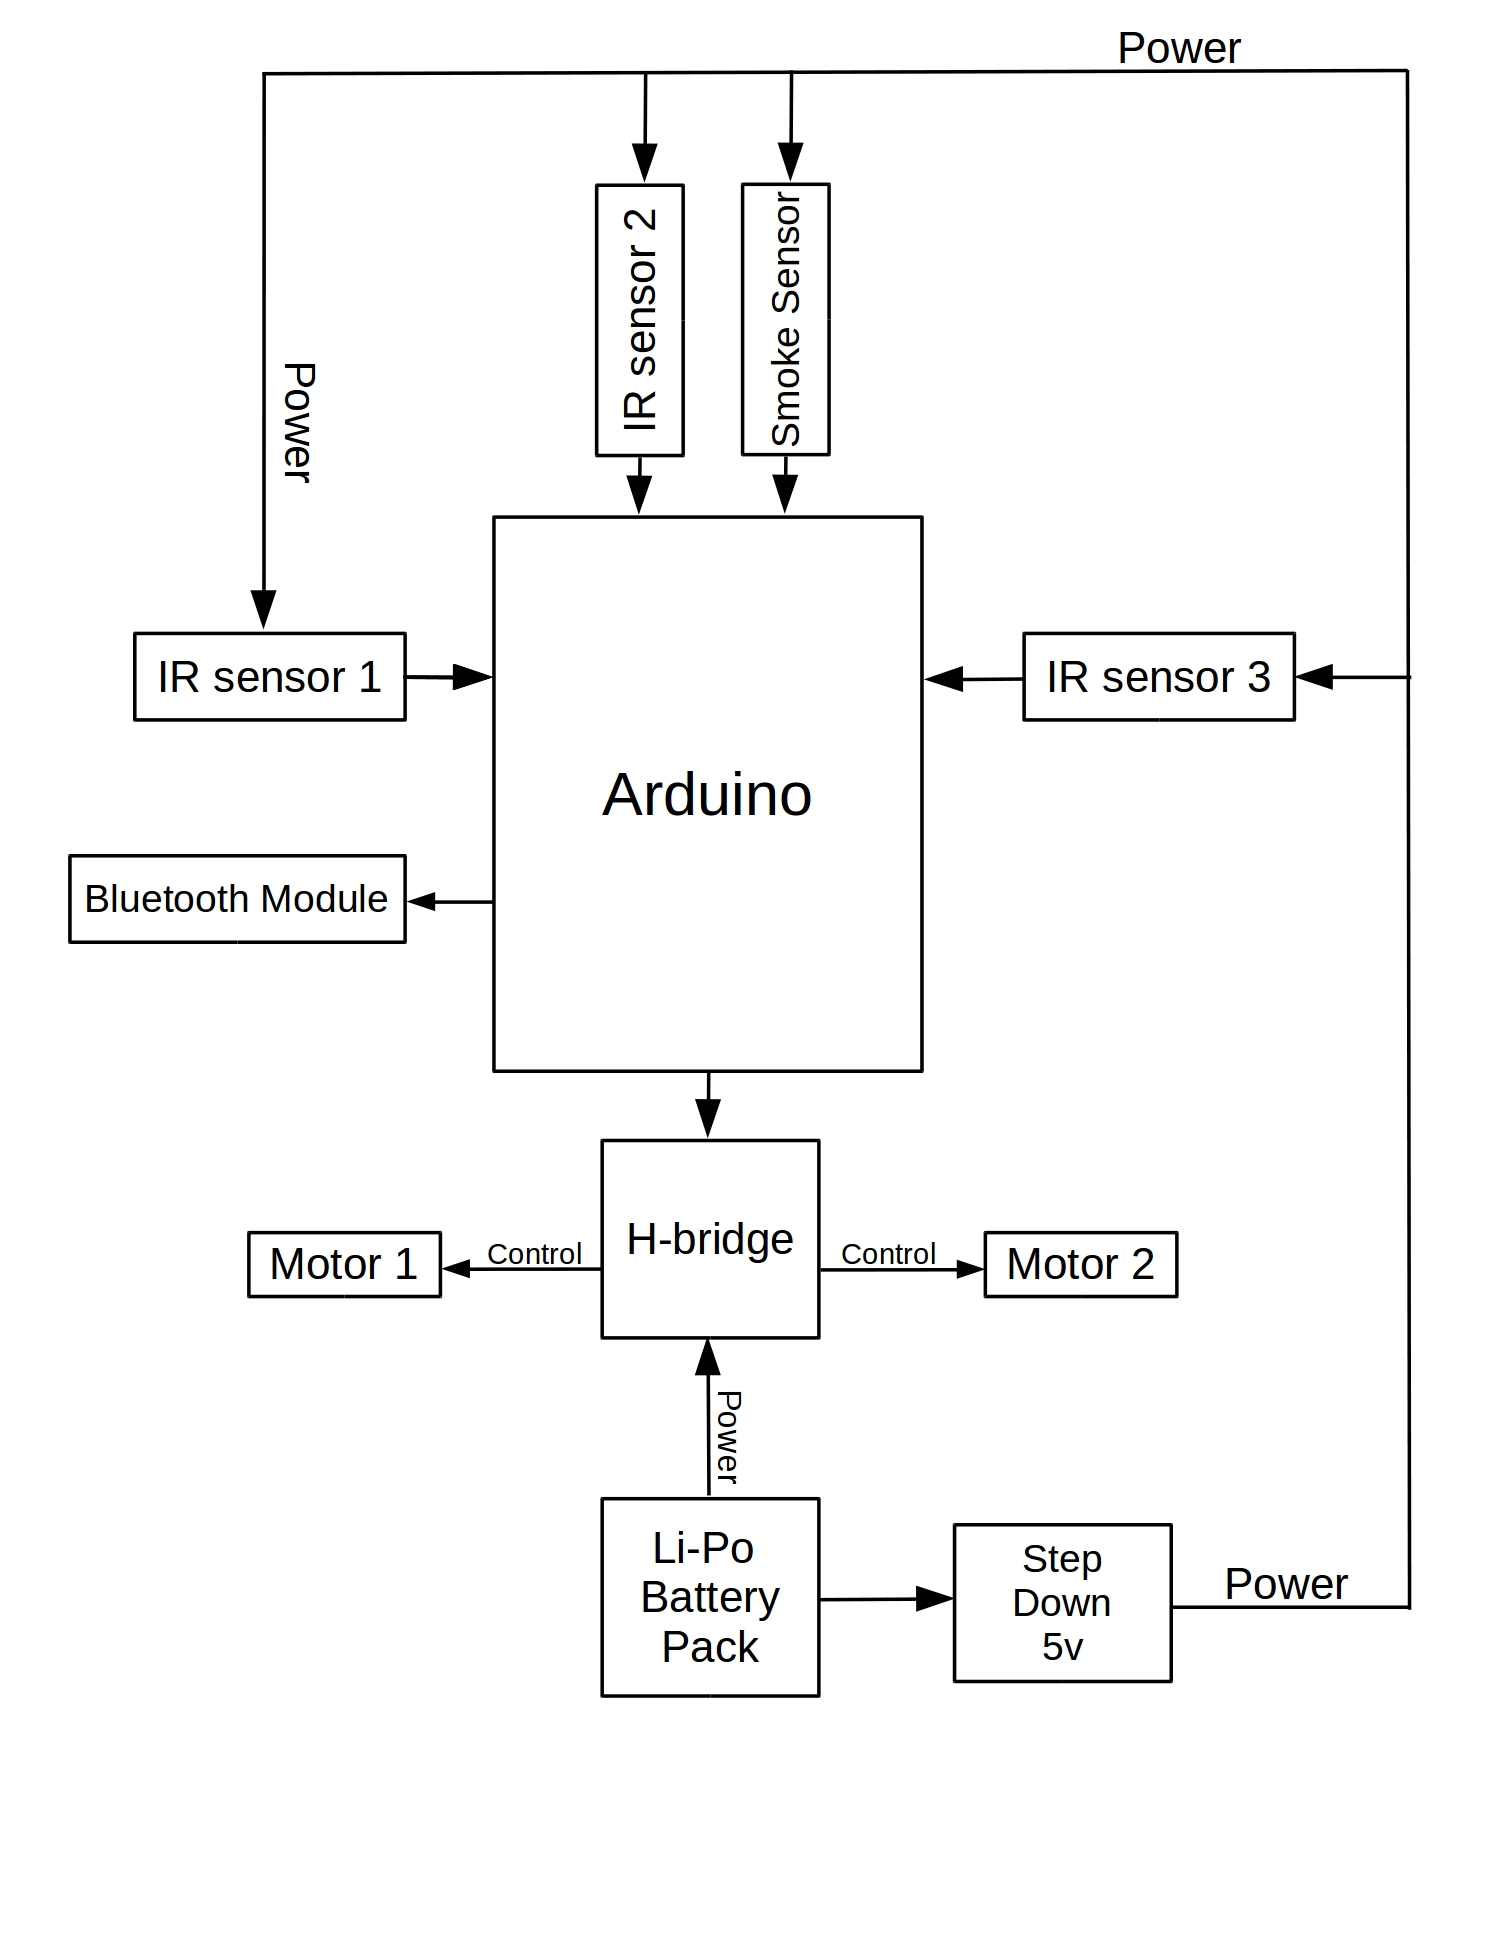
\includegraphics[scale=0.25]{bot1new.jpg} 
\caption{Schematic Representation of the first Robot}
 \end{figure}
\subsubsection{Second Robot}
The second robot is not much different from the first one. In the process of describing swarm intelligence, the second robot is intentionally made simpler than the first robot. So, tit does not contain the smoke sensor. Three IR sensors are attached just as in the first robot. Similarly, the arduino, bluetooth module and the motor controller are also attached in a similar way.The schematic is shown below:
\begin{figure}[h]
\center
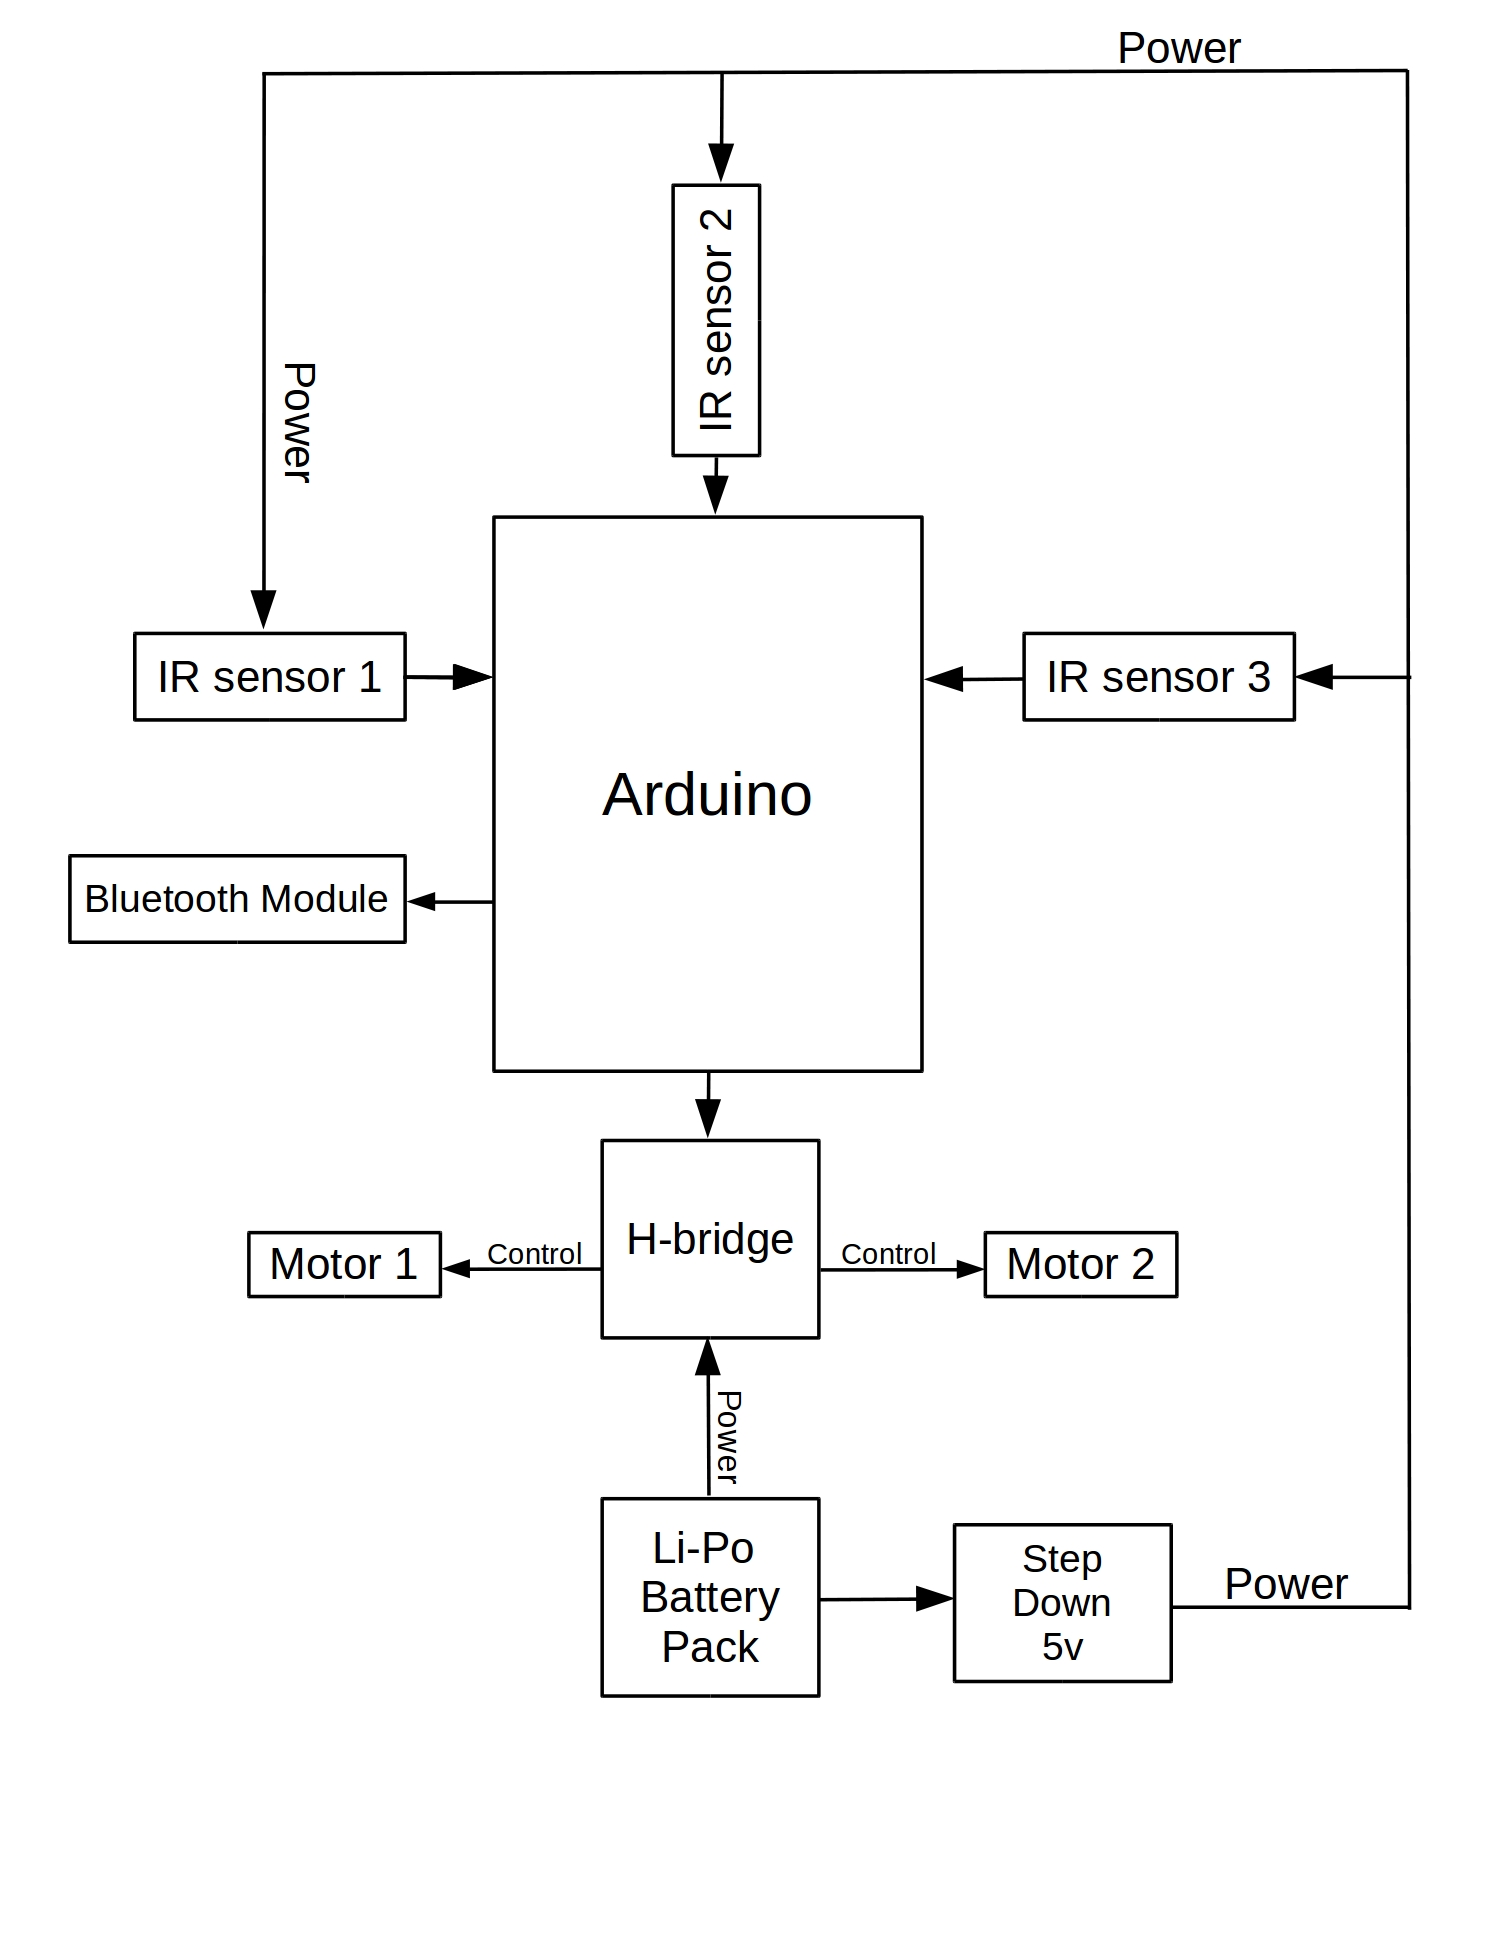
\includegraphics[scale=0.25]{bot2new.jpg} 
\caption{Schematic Representation of the second Robot}
 \end{figure}
\subsection{Interfacing Arduino UNO with L298N Dual H-Bridge motor controller}
Common Ground technique was applied by connecting the GND terminal of the UNO's to the ground socket of the motor controller. The supply to the UNO was provided via the 5v output socket of the motor controller and the motor controller was powered with Lithum Polymer battery.\\
For the interfacing of Arduino UNO with the L298N, the following pin configurations were done:
 
\begin{table}[h]
\center
\begin{tabular}{ |p{3cm}|p{3cm}|p{3cm}| }
\hline
\multicolumn{3}{|c|}{PIN CONFIGURATION} \\
\hline
ARDUINO PIN& L298N PIN &Remarks\\
\hline
5(PWM) & IN4&Enable Motor B\\
\hline
6 & IN3&Enable Motor B\\
\hline
7 &IN2&Enable Motor A \\
\hline
8 &IN1 &Enable Motor A\\
\hline
9&ENB&Enables PWM signal for Motor B.\\
\hline
10(PWM)& ENA& Enables PWM signal for Motor A \\
\hline
\end{tabular}
\caption{Pin Configurations of the interfacing of ArduinoUNO with L298N}
\end{table}


%\subsection{Locomotion of the Robot}
\subsubsection{Differential Kinematics}
\justify
The robot consists of two drive wheels mounted on a common axis, that is, it uses differential kinematics. Each wheel can be independently driven either forward or backward. While we vary the velocity of each wheel, for the robot to perform rolling motion, the robot rotate about a point that lies along their common left and right wheel axis. The point that the robot rotates about is known as the ICC - Instantaneous Center of Curvature.\\
\begin{figure}[h]
\center
\includegraphics[scale=0.75]{differential2.png}    
\caption{Arrangement for Differential Drive Kinematics}
\end{figure}
\justify 
By varying the velocities of the two wheels, we can vary the trajectories that the robot takes.
Because the rate of rotation $\omega$ about the ICC must be the same for both wheels, we can write the
following equations:\\
\begin{equation}
                                                                         		\omega(R+l/2)= Vr                                             
\end{equation}

 \begin{equation}
   \omega(R-l/2)= Vl   
 \end{equation}       
\justify
where l is the distance between the centers of the two wheels, Vr ; Vl are the right and left wheel
velocities along the ground , and R is the signed distance from the ICC to the midpoint between the wheels. At any instance in time we can solve for R and $\omega$:
\begin{equation}
                                                                         		                                                        R= l/2 (Vl+ Vr)/(Vl-  Vr)                                                  
\end{equation}
\begin{equation}
                                                                      	                                                                 \omega= ( Vr-Vl)/l                                                    	                                                      \end{equation}
\justify
There are three interesting cases with these kinds of drives.\\
\justify
\begin{enumerate}
\item If Vl = Vr, then we have forward linear motion in a straight line. R becomes infinite, and there
is effectively no rotation - $\omega$ is zero.
\item If Vl = -Vr, then R = 0, and we have rotation about the midpoint of the wheel axis, we rotate
in place.
\item If Vl = 0, then we have rotation about the left wheel. In this case R = l/2. Same is true if Vr = 0.
\end{enumerate}
\subsubsection*{Operation of H-Bridge:}
The basic operating mode of an H-bridge is fairly simple: if Q1 and Q4 are turned on, the left lead of the motor will be connected to the power supply, while the right lead is connected to ground. Current starts flowing through the motor which energizes the motor in (let’s say) the forward direction and the motor shaft starts spinning.
\begin{figure}[h]
\center
\includegraphics[scale=0.6]{photos/13281783_10154154713090270_1743784099_n.png} 
\caption{Current flowing in the forward direction}
\end{figure}
\justify
If Q2 and Q3 are turned on, the reverse will happen, the motor gets energized in the reverse direction, and the shaft will start spinning backwards.\\
\newpage
\begin{figure}[h]
\center
\includegraphics[scale=0.6]{photos/13285612_10154154713070270_1233792274_n.png} 
\caption{Current flowing in the backward direction}
\end{figure}
\justify
In a bridge, both Q1 and Q2 (or Q3 and Q4) should never be closed at the same time. If done so, a really low-resistance path between power and GND is created effectively short-circuiting power supply. This condition is called ‘shoot-through’ and is an almost guaranteed way to quickly destroy the bridge, or something else in the circuit.\\

\begin{figure}[h]
\center
\includegraphics[scale=1]{photos/13288876_10154154713075270_284275638_n.png} 
\caption{Occurrence of short-circuit}
\end{figure}
\justify
The H-bridge arrangement is generally used to reverse the polarity/direction of the motor, but can also be used to 'brake' the motor, where the motor comes to a sudden stop, as the motor's terminals are shorted, or to let the motor 'free run' to a stop, as the motor is effectively disconnected from the circuit. The following table summarizes operation, with Q1-Q4 corresponding to the diagrams above.\\
\begin{table}[h]
\begin{center}
\begin{tabular}{ |c|c|c|c|c| } 
 \hline
 Q1 & 	Q2 & Q3&Q4&RESULT\\ 
 \hline
 1 & 0 & 0 &1& Motor moves right \\ 
 \hline
 0 &  1&  1&0& Motor moves left \\ 
\hline
 0 & 0 & 0 & 0 & Motor coasts \\
\hline
 0&1&0&1&Motor brakes  \\
\hline
1&0&1&0&Motor brakes \\
\hline
1&1&0&0& Short Circuit\\
\hline
0&0&1&1& Short Circuit \\
\hline
1 &1&1&1& Short Circuit\\
 \hline
\end{tabular}
\caption{Operation of an H-bridge}
\end{center}
\end{table}
\newpage
\subsubsection*{PWM and H-Bridge for the operation of DC motor}
For the generation of PWM, analogWrite and digitalWrite functions are used in Arduino.
analogWrite controls speed and digitalWrite controls direction of DC motor.
DC motors normally have just two leads, one positive and one negative. If these two leads are directly connected to a battery, the motor will rotate. If you switch the leads, the motor will rotate in the opposite direction.\\
To control the direction of the spin of DC motor, without changing the way that the leads are connected, a circuit called an H-Bridge can be used. \\
We have used L298N H-Bridge IC. The L298N can control the speed and direction of DC motors and stepper motors and can control two motors simultaneously. Its current rating is 2A for each motor. So, heat sinks are used.\\
\newpage

\newpage
\subsection{Maze Traverse}
The job of the first agent is to traverse the maze and to generate the payload which carries all the information that has been collected by the first agent regarding the paths followed by it. The payload will then be transferred to the second robot via Bluetooth.\\
The second robot then decodes the payload and calculates the most optimal path to the destination.\\
For the purpose of maze traversal Left wall following algorithm is used.
\subsubsection{Left wall following algorithm}
This algorithm works on the basis that a maze solver will not be lost and will reach a different exit if there is any, by keeping one hand in contact will the left wall of the track. The maze solver, the first agent of the swarm in our case will always follow the left wall of the track and traverses all the tracks of the maze until it detects the target. At every junction of tracks the decision for the bots next turn is made based on which is the facing direction of the robot and determining the left side of the track. \\
The decision made by the bot on every junction is summarized in the table below:
\begin{table}[h]
\begin{center}
\begin{tabular}{ |c|c|c|c|c| } 
 \hline
 Facing & 	1 Priority & 2 priority &3 Priority&4 Priority\\ 
 \hline
 North& W &N  &E&S  \\ 
 \hline
 South & E &  S&W&N \\ 
\hline
 East&  N  & E &S & W \\
\hline
 West&S&W&N&E  \\
\hline
\end{tabular}
\caption{Decision priorities of left wall follower algorithm}
\end{center}
\end{table}
\subsubsection{Algorithm Flowchart}
\begin{figure}[h]
\center
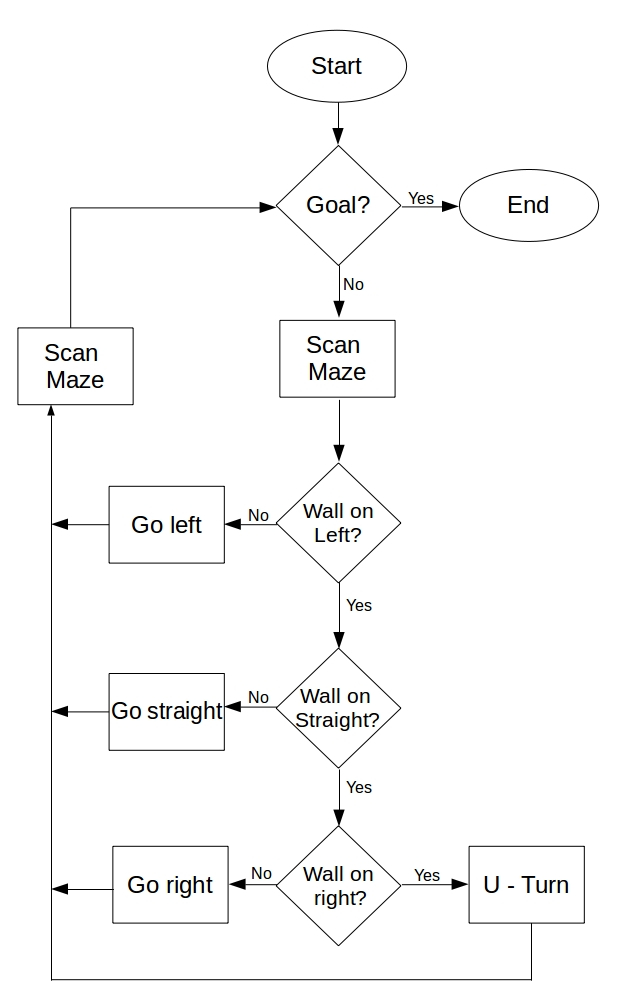
\includegraphics[scale=0.5]{flowchartnew.jpg}  
\caption{Flow-chart of left wall follower algorithm}
\end{figure}
\subsubsection{Implementation}
The leftwall following algorithm can be implemented using various models.\\ 
The model we are using contains three sensors placed at the left, right and the front facing of the robot as shown in the figure.
\begin{figure}[h]
\center
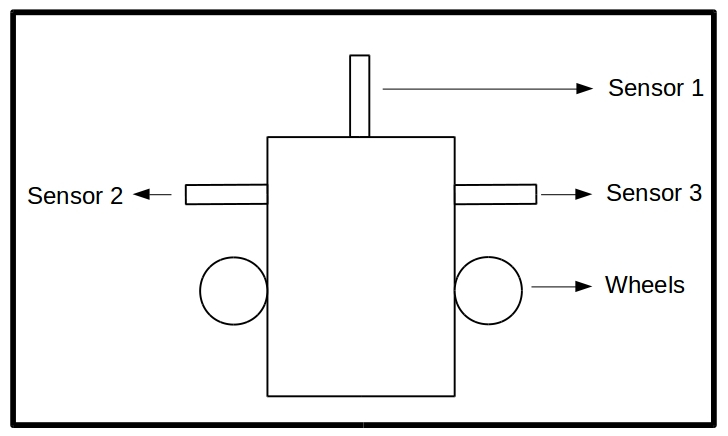
\includegraphics[scale=0.5]{bot.jpg}  
\caption{Implementation of left wall-follower algorithm}
\end{figure}
\justify The decisions are made by the robots based on the output of the all three sensors. At every junction point, which are characterized by the presence of two more than two options that the robot has to consider, the robot has to decide whether to go right or left or straight.\\
The junctions that the robot may encounter are the instants where the robot has to make the decision as to which direction to continue due to the presence of two or more options and the instants where the robot has to take a U turn. The various junctions that can be present in the maze are shown in the figure below:\begin{figure}[h]
\center
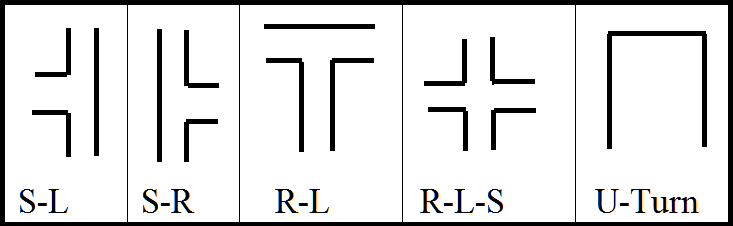
\includegraphics[scale=0.7]{Capture4.PNG} 
\caption{Possible junctions of a maze}
\end{figure}
\justify The first agent, irrespective of the position of the target always prefers the left path over straight path and straight path over the right one. The second robot however has to eliminate the mistakes made by the first robot so as to avoid reaching to the dead ends.\\
The decision made and the corresponding sensor values at the junctions are summarized in the table below:
\begin{table}[h]
\begin{center}
\begin{tabular}{ |c|c|c|c| }
\hline 
Sensor 1 (Front)&	sensor 2 (Left)	&sensor 3 (Right)&	Decision\\
\hline
High&	low	&low& 	Go left\\
\hline
Low	&low	&high&	Go left\\
\hline
Low&	high&	low	&Go straight\\
\hline
High&	high&	high&	U-turn\\
\hline
\end{tabular}
\caption{Decision made and the corresponding sensor values}
\end{center}
\end{table}
In the above table, the sensor value 'low' means there is no obstacle in the path of the sensor facing and it is clear to go whereas the sensor value 'high' means that the path faced by the sensor is blocked by the obstacles.\\
Using this algorithm the robot traverses the whole maze , through the every possible paths and reaching every junctions and the dead ends until it reaches the target, which in our case will be sensed by the smoke sensor. Further discussion on the target detection will be discussed in the later sections.\\
Now all the information gathered by the first agent about the maze structure and the decisions made at every junctions needs to be molded into the appropriate payload which can be sent through the Bluetooth module HC-05 to the second robot.\\
The discussion on how this is carried out in our project is included in the following sub-section.
\subsubsection{Payload generation}
The payload generation for the Bluetooth communication can be done by encoding the distance covered by the robot between the points of interest, but for the implementation of this model we needed an encoder.\\
Due to the unavailability of the encoders in the Nepali market and the time constraints we had, we came up with another implementation model which encodes the decision made at every junction.\\
In this implementation model, first all the junctions are assigned a number which gives the position of the junction. Then the decisions made at each junction are sent as the string of encoded binary data which are later decoded by the second robot in course of finding the most optimal path.\\
All the possible decisions which can be made at any junction are encoded using 3-bit as shown in the table below:\\
\begin{table}[h]
\begin{center}
\begin{tabular}{ |c|c| }
\hline 
Decision&	Bits\\
\hline
Left	&001\\
\hline
Straight&	010\\
\hline
Right	&011\\
\hline
U-turn	&101\\
\hline
\end{tabular}
\caption{Encoded binary values of the decisions made by the robot}
\end{center}
\end{table}
\justify The reason behind using 3-bit encoding when only four decisions can be made will be discussed in the decoding section.\\
We considered the following maze:
\newpage
\begin{figure}[h]
\center
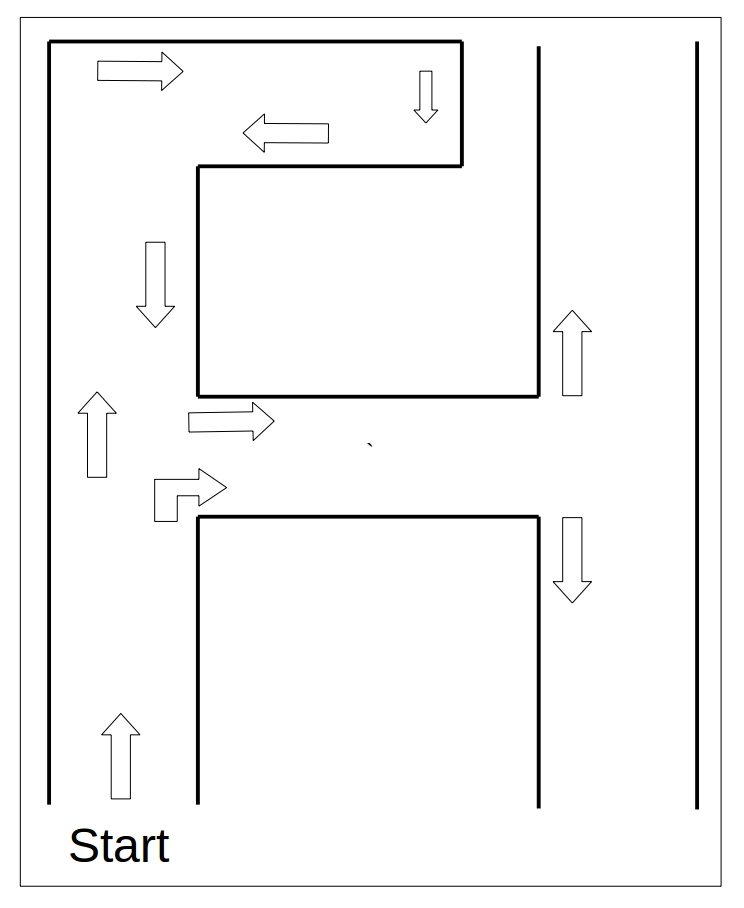
\includegraphics[scale=0.5]{mazebold.jpg}   
\caption{Example maze for illustration}
\end{figure}
\justify Now the robot starts from the starting positions and goes straight until it finds out that there are two possible paths it can continue on. At this point the first robot makes the decision based on the priorities set by the left wall following algorithm. And every decisions made by the robot is kept as the encoded binary bits in the memory.\\
In the above maze, the first robot reaches the first junction and decides to continue going straight which will then be represented as '010' and same process will be repeated until the target is reached.\\
 When the target is reached we will have a long bit string which will represent the decisions made at every junction on the group of every 3-bit of the string. The string will later be decoded by the second robot to know the decisions made by the first robot.
\subsubsection{Decoding} 
The message received by the second robot would contain a string of zeros and ones. The message encoded in this string of bits needs to be decoded to get information about the maze.\\
Let us represent the string received from the first robot as below:
\begin{table}[h]
\begin{center}
\begin{tabular}{ |c|c|c|c|c|c|c|c|c| }
\hline 
A0&	A1&	A2&	A3&	A4&	A5&	-&	-&	An\\
\hline
\end{tabular}
\caption{The representation of Bit String}
\end{center}
\end{table}
\justify A0 till An  being the individual bits of the string.\\
Each group of three bits starting from A0 would be the decision made by the first robot at the junctions  as to whether it took left, right, straight or U-turn from the junction using the encoding table previously presented.\\
The string is treated as the string of quanta of 3-bits.\\
In the case of the maze of figure ,the message sent by the first robot will be:
\begin{figure}[h]
\center
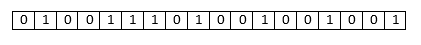
\includegraphics[scale=1]{bit.PNG}   
\caption{Received bit string for the above given maze}
\end{figure}
\justify The second robot receives first three bits and decodes that the first robot had taken straight from the first junction. Similarly it decodes the other bits and finally the decoded message sent by the first robot is shown as:
\newpage
\begin{table}[h]
\begin{center}
\begin{tabular}{ |c|c|c|c|c|c| }
\hline 
S	&R&	U&	L&	L&	L\\
\hline
\end{tabular}
\caption{The decisions made at junctions}
\end{center}
\end{table}
\justify The presence of 'U' in the message indicates that the first robot had to return to previous junction where it had taken the wrong alternative. So, every time the second robot finds 'U' in the message it eliminates the preceding bits until it encounters the junction. The junctions would be characterized by the presence of more than two options for the robot to continue.\\
If the bits  A\textsubscript{m-1} , A\textsubscript{m}, A\textsubscript{m+1} are decoded as the U-turn then the second robot eliminates the preceding bits that is  A\textsubscript{m-2},A\textsubscript{m-3},…  until it reaches the junction with more than two options i.e.  a Junction.\\ 
The reason for using 3-bits to encode just four possible decisions is, during the decoding  while the second robot has to eliminate the undesired decisions it will replace them with bits '000' so the use of 2-bit encoding would have caused problem on eliminating the undesired message bits. 

\subsection{Communication and Connection}
The main goal of this project was to develop a robust system of communication between both
robots for use in future projects. The communication scheme that was eventually chosen was Bluetooth, a proprietary wireless standard invented in 1994 by L.M. Ericsson.\\
Bluetooth makes it very straight forward to establish a direct serial link between two robots,
making it possible to avoid extra infrastructure related to the communication medium. Without any added infrastructure, it is possible to move the robot system from one location to
another. Another distinct advantage is the Bluetooth enabled robot’s ability to communicate
with any other Bluetooth technology, including printers, and wireless phones, to name a few.
A major disadvantage of Bluetooth is its limited range of approximately 30 feet, as opposed
to the 802.11x typical range of about 300 feet. While this was not an issue with the current
project because of the small size of the task area, when working in larger arenas, Bluetooth
type communication would require the robots to remain much closer together. However, it is
quite possible to extend the range of the system by using robots to relay messages between
one another.
\subsubsection{Setting up a wireless connection between two Arduinos}
Bluetooth works by having a slave and a master. The slave modules can not initiate a connection to another Bluetooth device, but can accept connections, the master can be be set to either master or slave mode, when in master mode the module can initiate a connection to other devices. 
For the purpose of communication between the two arduinos, we need to configure one HC-05 as master and the other as slave. For this purpose, arduino IDE is used.
\subsubsection*{Configuring the HC-05 as Slave}
By default all HC05 modules are SLAVEs.\\
Before connecting the HC05 module , we uploaded an empty sketch to Arduino. This bypasses the Boot loader of UNO $\&$ the Arduino is used as USB-UART converter.
\begin{flushleft}
void setup() \big\{ \big\}\\
void loop() \big\{ \big\}\\
\end{flushleft}
\begin{table}[h]
\begin{center}
\begin{tabular}{ |c|c| }
\hline 
 ARDUINO     &   HC05\\
 \hline
Rx(pin0 )  &Rx\\
\hline
Tx (pin1) &   Tx\\
\hline
+5v     & VCC\\
\hline
GND     & GND\\
\hline
+3.3V  & KEY\\
\hline
\end{tabular}
\caption{The connection between HC-05 and arduino UNO for slave configuration}
\end{center}
\end{table}
\justify After uploading this empty sketch,USB power was removed from Arduino $\&$ the following connections were done with HC05 Slave as shown in the above table\\
The USB cable power to Arduino was provided and subsequently, the HC05 module enters the Command mode with Baud Rate 38400.
By opening the Serial Monitor of Arduino, the HC-05 can be configured as slave.\\
The ROLE of the module can be known by typing  AT+ROLE?\\
The following AT command setups the HC-05 module as a slave.
\begin{equation}
AT+ROLE=0
\end{equation}
\justify Here are some screenshots of the Serial Monitor Window displaying the slave module setup.
%-------screenshots-----------------------------
\newpage 
\subsubsection*{MASTER Module setup}
The bluetooth module HC-05 can be provided the role of master in a similar way as the slave module setup i.e. Using AT commands.\\
Before connecting the HC05 module , we uploaded an empty sketch to Arduino in a similar fashion as done for the slave module setup. 
\begin{flushleft}
void setup() \big\{
  \big\}\\
void loop() \big\{
\big\}
\end{flushleft}
\justify The connections were as similar as the slave module setup as tabulated below:
\begin{table}[h]
\begin{center}
\begin{tabular}{ |c|c| }
\hline 
 ARDUINO     &   HC05\\
 \hline
Rx(pin0 )  &Rx\\
\hline
Tx (pin1) &   Tx\\
\hline
+5v     & VCC\\
\hline
GND     & GND\\
\hline
+3.3V  & KEY\\
\hline
\end{tabular}
\caption{The connection between HC-05 and arduino UNO for master configuration}
\end{center}
\end{table}
\justify The following AT command setups the HC-05 module as a master.
\begin{equation}
AT+ROLE=1
\end{equation}
\justify And now to actually connect to the SLAVE switch off both the modules. We removed the KEY connection from master and the module was reset by removing the power $\&$ connecting back.\\
On powering back the MASTER ,the Slave gets paired with it automatically which can be verified by the LEDs on board as the LEDs of both the modules start blinking at the rate of a blink every two seconds. The paired devices are remembered even after disconnecting power.\\
Now these two modules replaced the physical serial connection of the project.\\
Bluetooth networks (commonly referred to as piconets) use a master/slave model to control when and where devices can send data. In this model, a single master device can only be connected to up to one other slave device. Any slave device in the piconet can only be connected to a single master.\\
The master coordinates communication throughout the piconet. It can send data to the slave and request data from it as well. Slave is only allowed to transmit to and receive from the master.\\
\newpage
%===============================================
\section{RESULT}
\subsection{Path traversal by the first robot}
From the initial position, the first robot began to traverse the maze and the required decisions at the junctions were taken on the basis of the priorities  provided by our left wall following algorithm and subsequently, the first robot traveled the entire maze and ultimately the target was detected.\\
The path followed by the robot is shown in the figure below: 
\begin{figure}[h]
\center
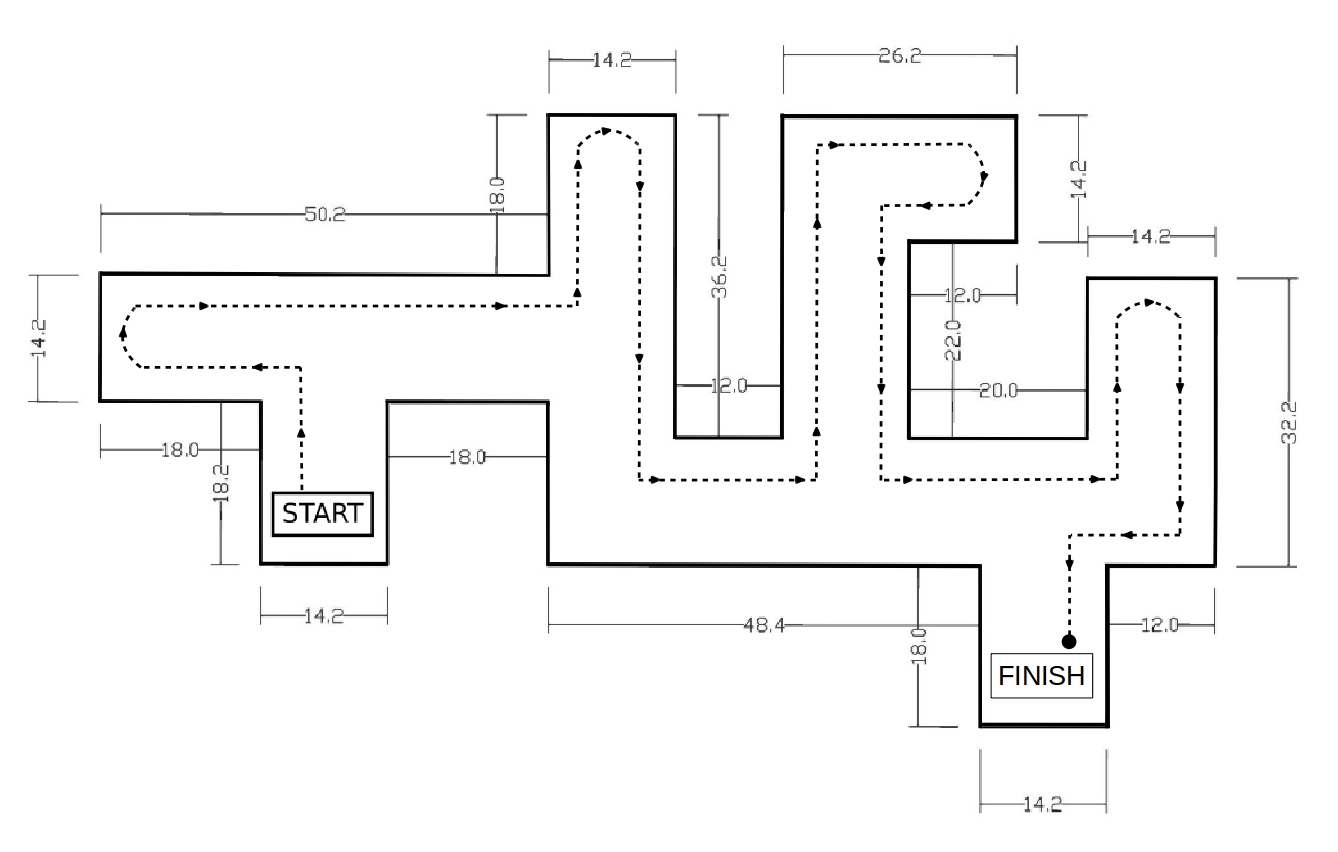
\includegraphics[scale=0.3]{mazetraverse_newnew.jpg} 
\caption{The path followed by the first robot}
\end{figure}
\subsection{Target Detection}
Eventually, the final target for the first robot to detect was chosen to be smoke.  The travelling robot does not know the location of the target which was present somewhere in the maze and subsequently detected the target using MQ-2 gas sensor which was implemented in the robot. \\
MQ-2 Gas Sensor works on the principle “The greater the gas concentration, the greater the output voltage" .Thus, the sensor analog output voltage was read and when it reached/crossed a certain threshold, the target detection decision was taken as positive and subsequently the first robot was stopped for any locomotion thereafter.
\begin{figure}[h]
\center
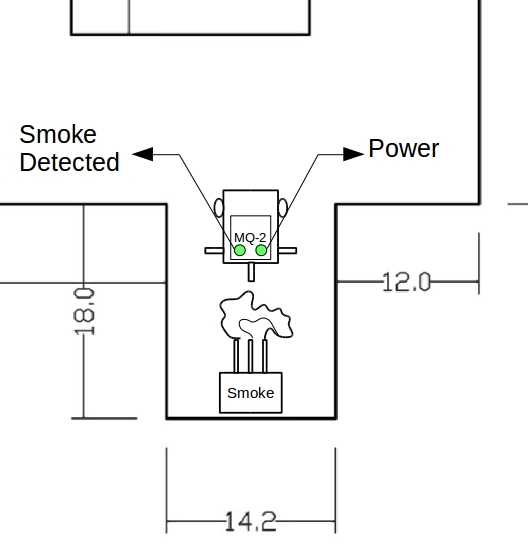
\includegraphics[scale=0.5]{part4_1_final.jpg} 
\caption{Target Detection by the first robot through MQ-2 Smoke Sensor}
\end{figure}
\subsection{Bluetooth Communication}
Both the LEDs of the master and slave setup HC-05 blinked at the rate of two fast blinks every two seconds. This indicated that both the master and slave modules were paired with each other.\\
The decisions taken at the junctions were then decode and were sent to the second robot via Bluetooth.\\ 
Thus, based upon the decoded message, the second robot traversed the maze in the shortest path possible. \\
The decisions made by the first robot at the junctions is shown in the figure below:\\
\newpage
\begin{figure}[h]
\center
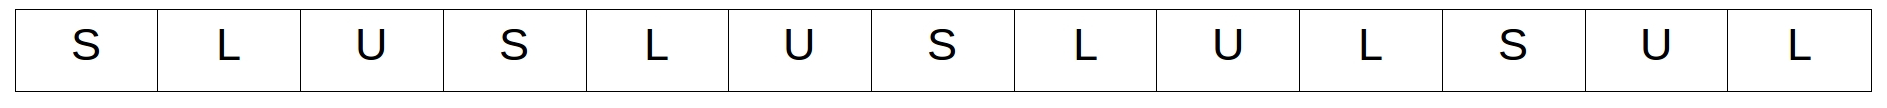
\includegraphics[scale=0.25]{packet_new.jpg} 
\caption{The decisions taken at the various junctions in the above given maze}
\end{figure}
\justify The above decisions were then decoded and was sent to the second robot via the Bluetooth module for traversing the maze in the shortest path possible.\\
\justify The decoded decisions are shown in the table below:
\begin{table}[h]
\begin{center}
\begin{tabular}{ |c|c|c|c|c| }
\hline 
S&R&R&S&R\\
\hline
\end{tabular}
\caption{The decoded decisions sent to the second robot}
\end{center}
\end{table}
\begin{table}[h]
\begin{center}
\begin{tabular}{ |c|c|c|c|c| }
\hline 
S&STRAIGHT\\
\hline 
R&RIGHT\\
\hline 
L&LEFT \\
\hline 
U&U-TURN\\
\hline
\end{tabular}
\caption{S,R,L,U Notations}
\end{center}
\end{table}
\subsection{Path traversal by the second robot}
The second robot received the information/decision from the first robot and started traversing the maze. The junction in the maze was detected by a set of IR Sensors similar to that on the first robot.  Upon the arrival of the junction ,  the second robot took the desired decision that led the robot through the shortest path to the target.\\
The path followed by the second robot is shown in the figure below:
\newpage
\begin{figure}[h]
\center
 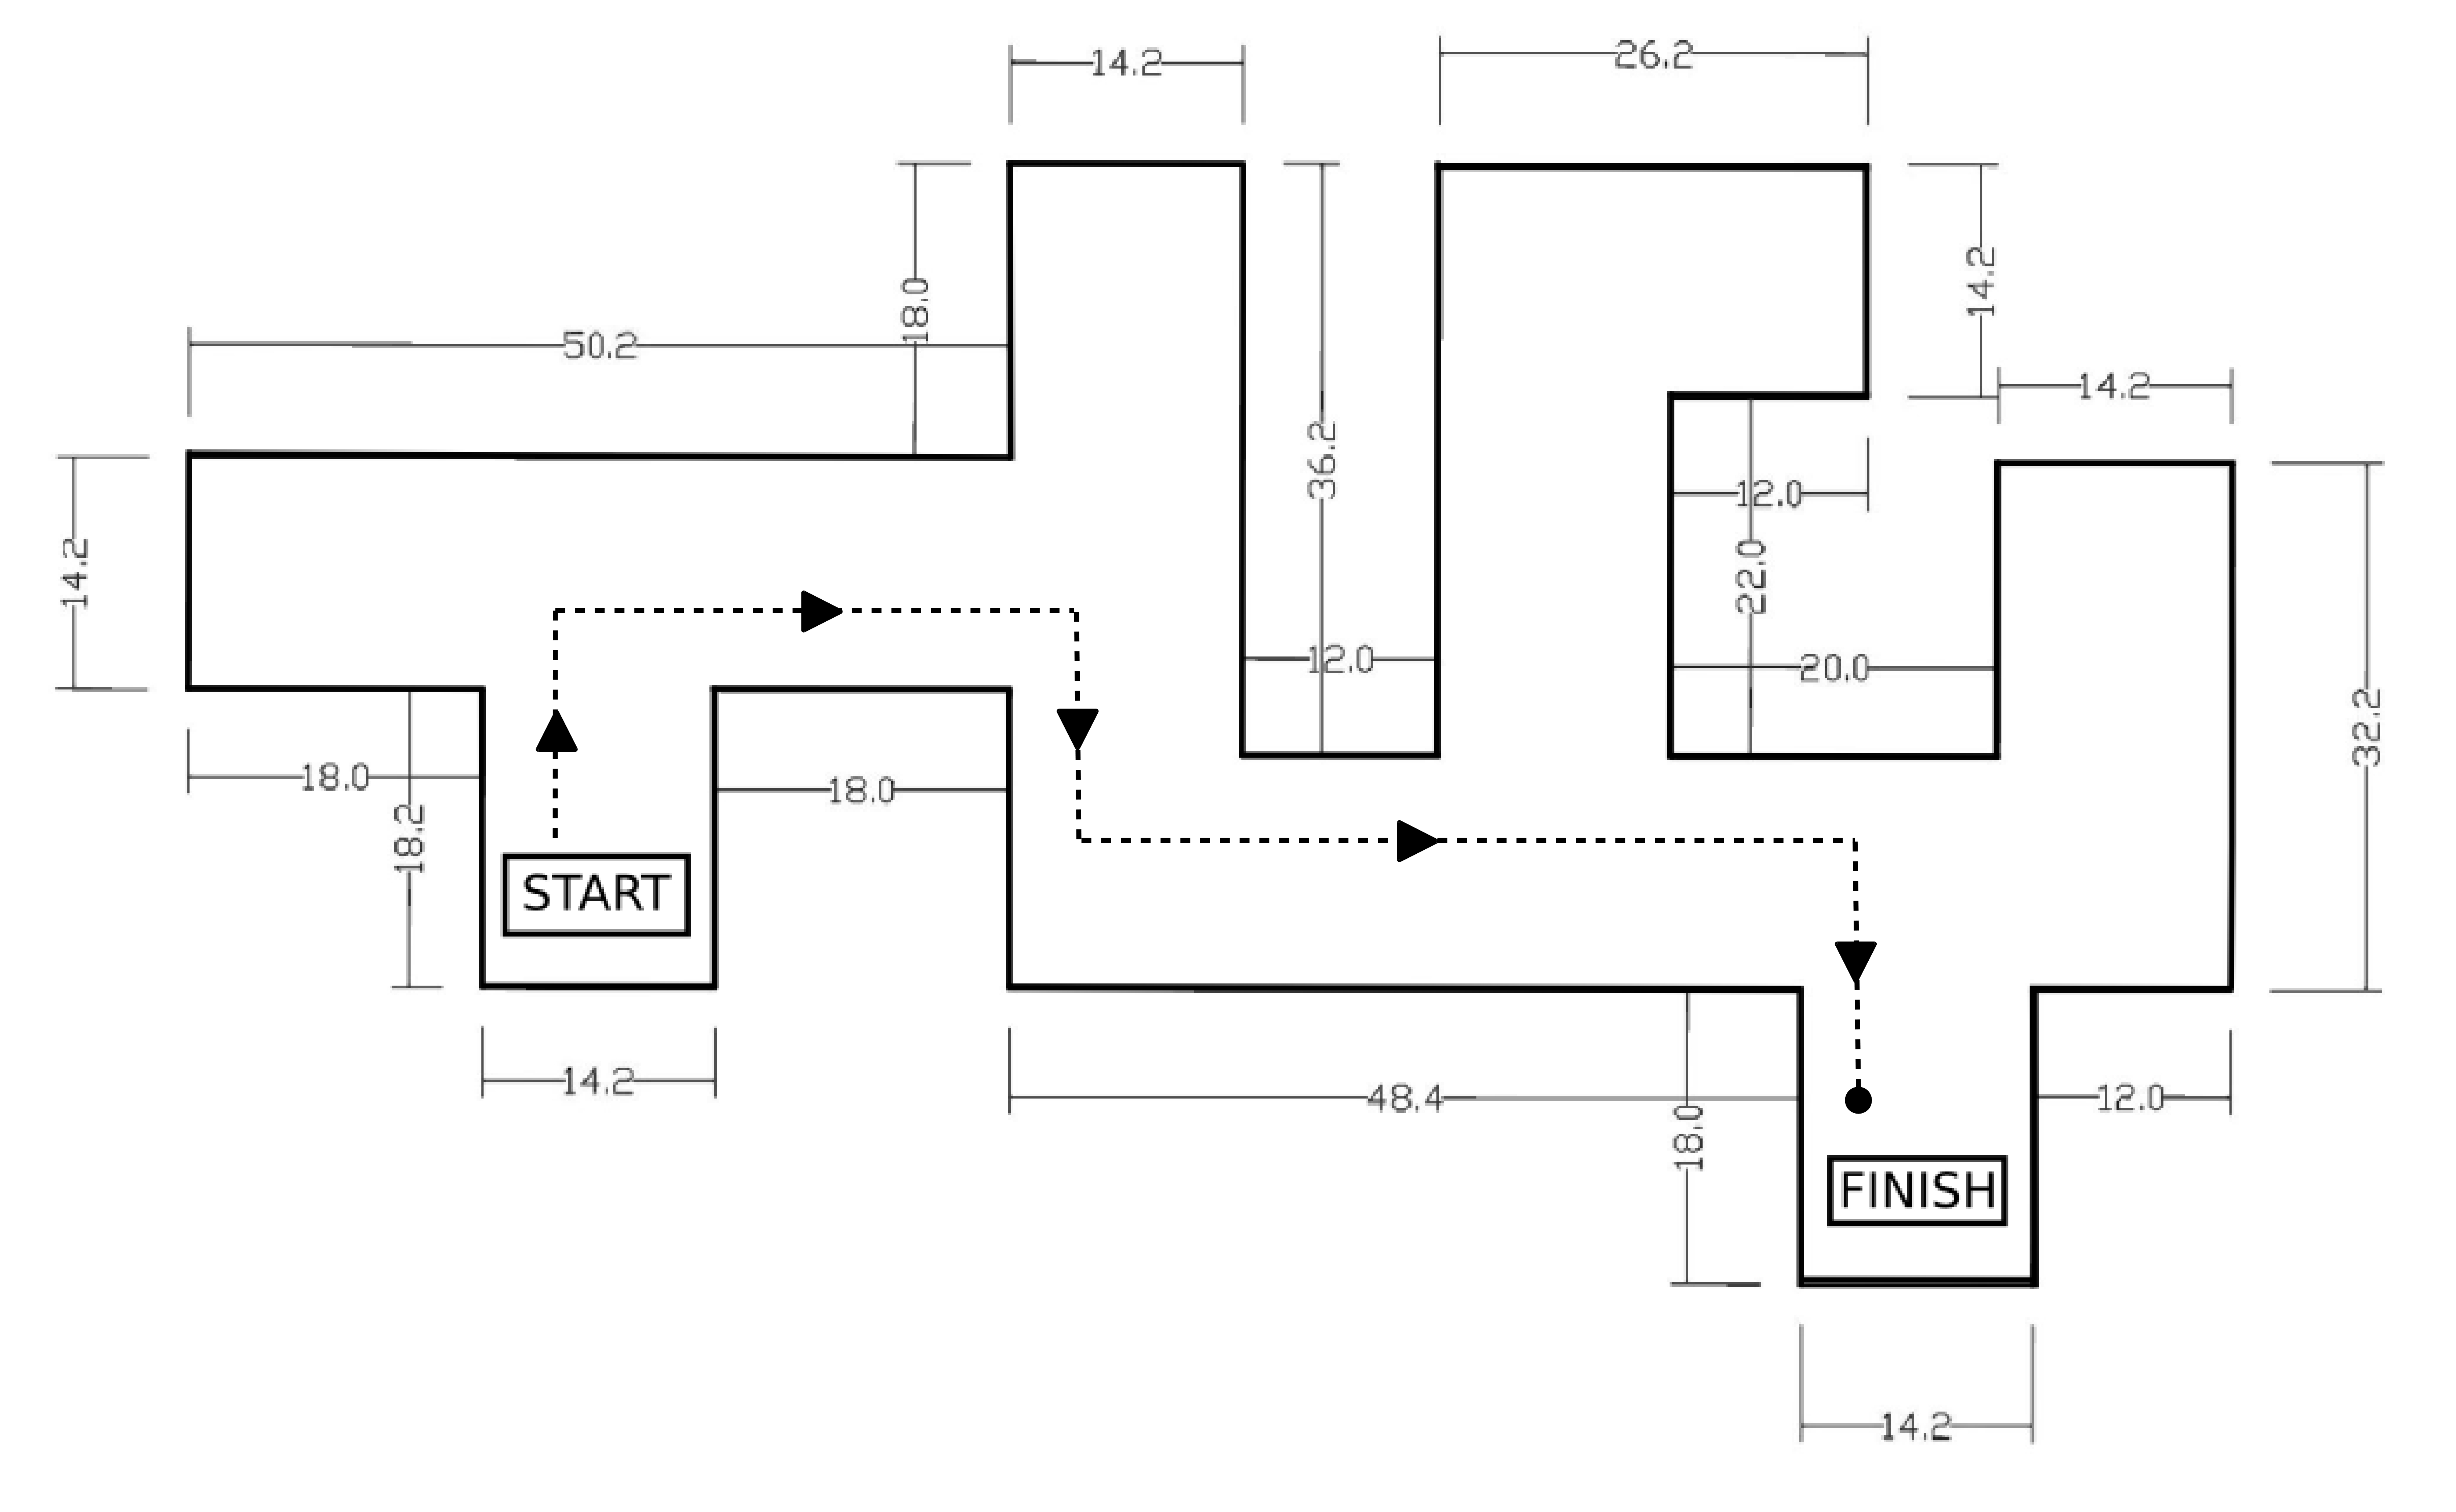
\includegraphics[scale=0.067]{mazetraverse_shortest_newnew.jpg} 
\caption{The shortest path followed by the second robot}
\end{figure}
%\subsection{PWM waveforms}
%For generating PWM waveforms, analogWrite function was used in the ATMEGA 328P microcontroller. It was then interfaced with H-Bridge to control the direction. By changing the direction of current flow in H-Bridge and interfacing it with Arduino, we have moved the robot in left, right, clockwise, anticlockwise and stopped it.  The motor was then connected with H-Bridge to change its direction. We have used pins 8, 9 ,6 and 5 of Arduino with IN1, IN2, IN3 and IN4 respectively of H-Bridge. The PWM waves were generated from  ENA (pin 10) and ENB (pin 9 ) of Motor 1 and 2 respectively.
%\begin{enumerate}
%\item When robot moved in clockwise direction
%\begin{figure}[h]
%\center
%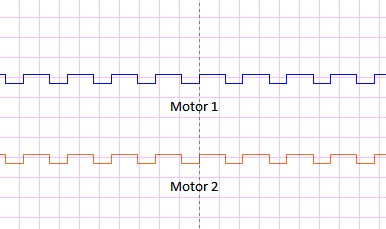
\includegraphics[scale=1]{pwm1_invert.jpg} 
%\caption{Waveforms of moor 1 and motor 2 in the clockwise direction}
%\end{figure}
%\item When robot moved in anti-clockwise direction
%\begin{figure}[h]
%\center
%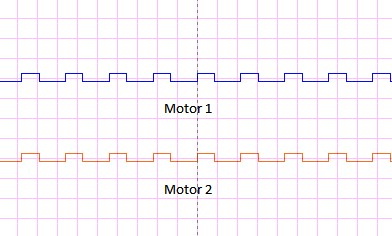
\includegraphics[scale=1]{pwm2_invert.jpg} 
%\caption{Waveforms of motor 1 and motor 2 in the anticlockwise direction}
%\end{figure}
%\item When motor moved in left direction
%\begin{figure}[h]
%\center
% 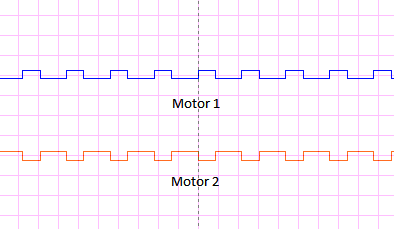
\includegraphics[scale=1]{leftd.png} 
%\caption{Waveforms of motor 1 and motor 2 in the left direction}
%\end{figure}
%\item When motor moved in right direction
%\begin{figure}[h]
%\center
%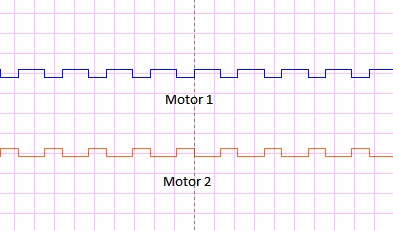
\includegraphics[scale=1]{rightd.png}   
%\caption{Waveforms of motor 1 and motor 2 in the right direction}
%\end{figure}
%\item When motor stopped\\
% For stopping the motor, all pins were set low, i.e, all IN1, IN2, IN3 and IN4 were 0. As all the pins were low so, no current was flown through the motor. No PWM value was given preventing the appearance of PWM waves.
%\end{enumerate}
\newpage
\section{DISCUSSION}
\subsection{Algorithm implementation}
As mentioned earlier in the above section, left wall following algorithm was implemented in the first robot in order to carry out the task of maze traversal. 
According to the aforementioned algorithm, the robot always tries to follow the left wall of the maze. Basically, the first step towards implementation of the algorithm was detection of the closest wall. \\
\begin{figure}[h]
\center
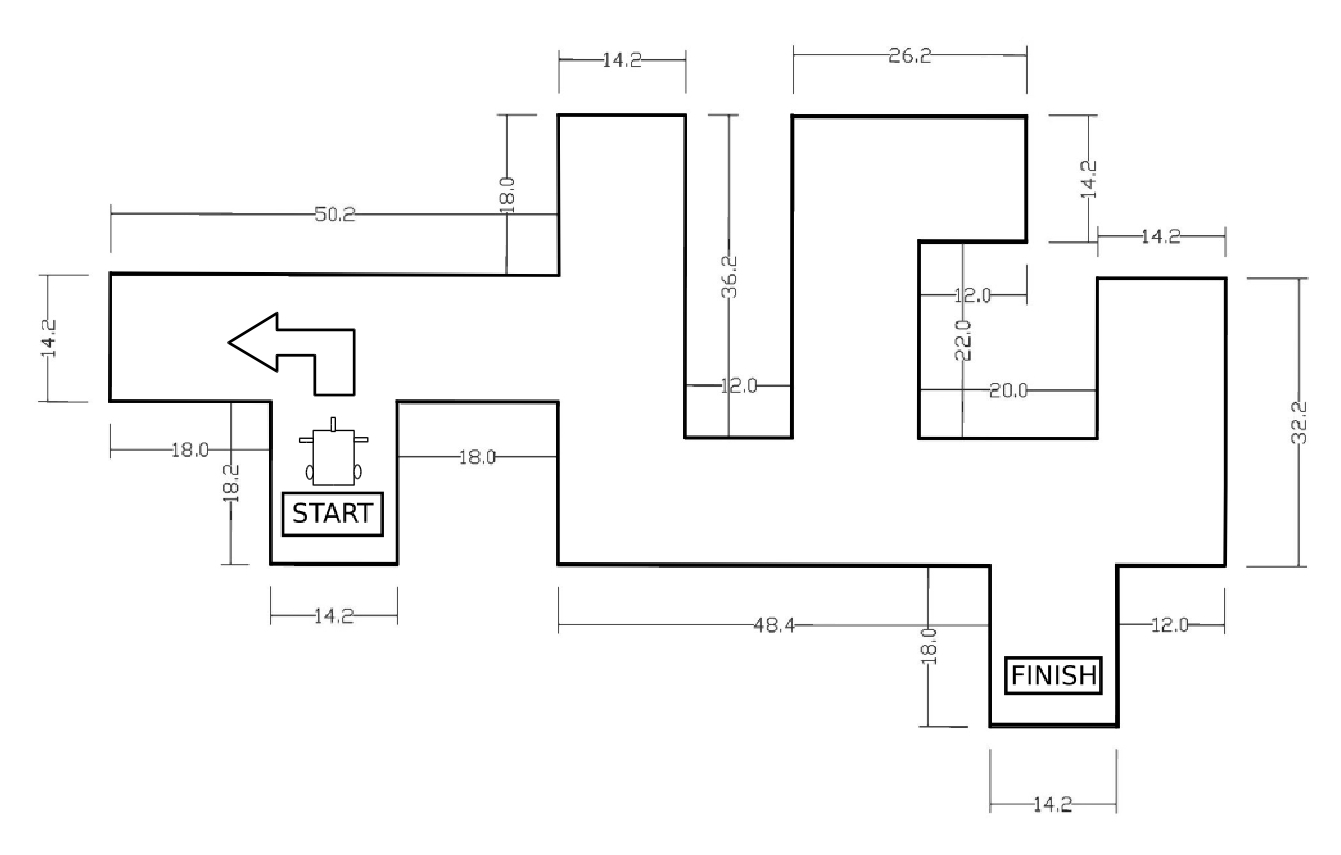
\includegraphics[scale=0.3]{part1_newnew.jpg}
\caption{Detection of the closest wall} 
\label{Firstplacementofthebot}
\end{figure}
\justify The robot followed the left wall until it encountered a junction where a decision had to be made. Based on this algorithm the robot turned left when there was an opening in the respective direction. In any condition that the left opening was blocked or there was a wall along the left side of the robot, the priority was transferred to the straight movement and it kept following the left wall until the next junction occurred. When both the left and front openings were blocked, the robot turned right provided there was an opening in that direction. Finally, when there was a blockade on all the three above mentioned sides viz. Left, straight and right, the robot decided to take a U-turn. 
Using this technique, the robot was able to traverse the maze up to the target point.\\
\begin{figure}[h]
\center
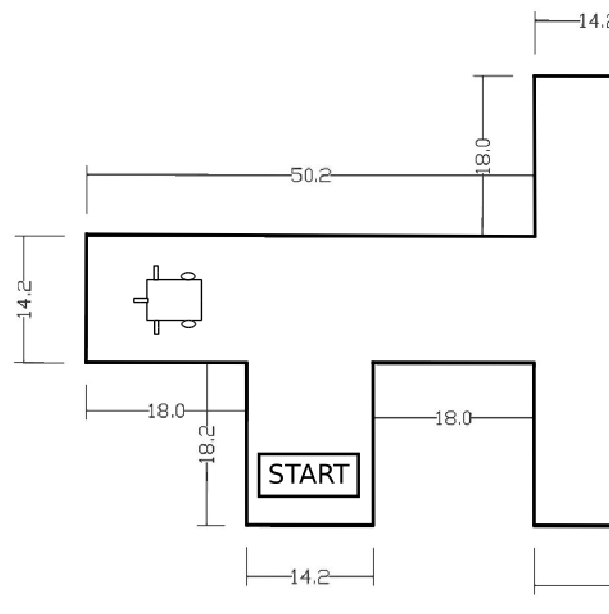
\includegraphics[scale=0.6]{part1_2new.jpg}
\caption{Robot following the left wall} 
\end{figure}
\justify From the above figure it can be seen that there is no any possible path for the robot's movement. Hence, it takes a U-turn as shown in the figure below.\\
\newpage
\begin{figure}[h]
\center
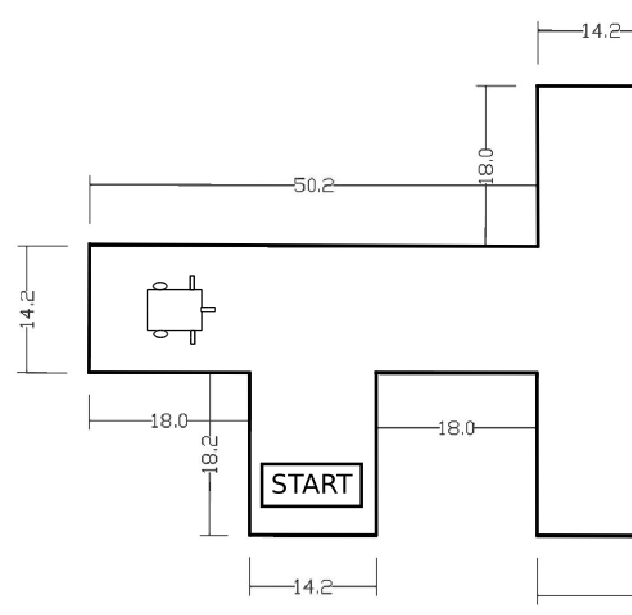
\includegraphics[scale=0.6]{part1_3new.jpg}
\caption{U-turn of the robot} 
\end{figure}
\subsection{Detection of the wall}
Detection of the wall was carried out through IR sensors. The IR sensor module FC-51 has a sensing range of up to 30cms. The left wall of the maze was detected by the IR sensor which was indicated by the LED present within the module. By adjusting the potentiometer of the sensor module, the IR was made to detect a wall at a distance of about 6-8 cms. Similarly, the sensors placed on the front and right side of the robot were able to successfully detect the respective walls.\\
The following image shows the working of the IR sensor module along the left wall.\\
\newpage
\begin{figure}[h]
       \begin{center}
       
       \begin{subfigure}[b]{0.5\textwidth}
                 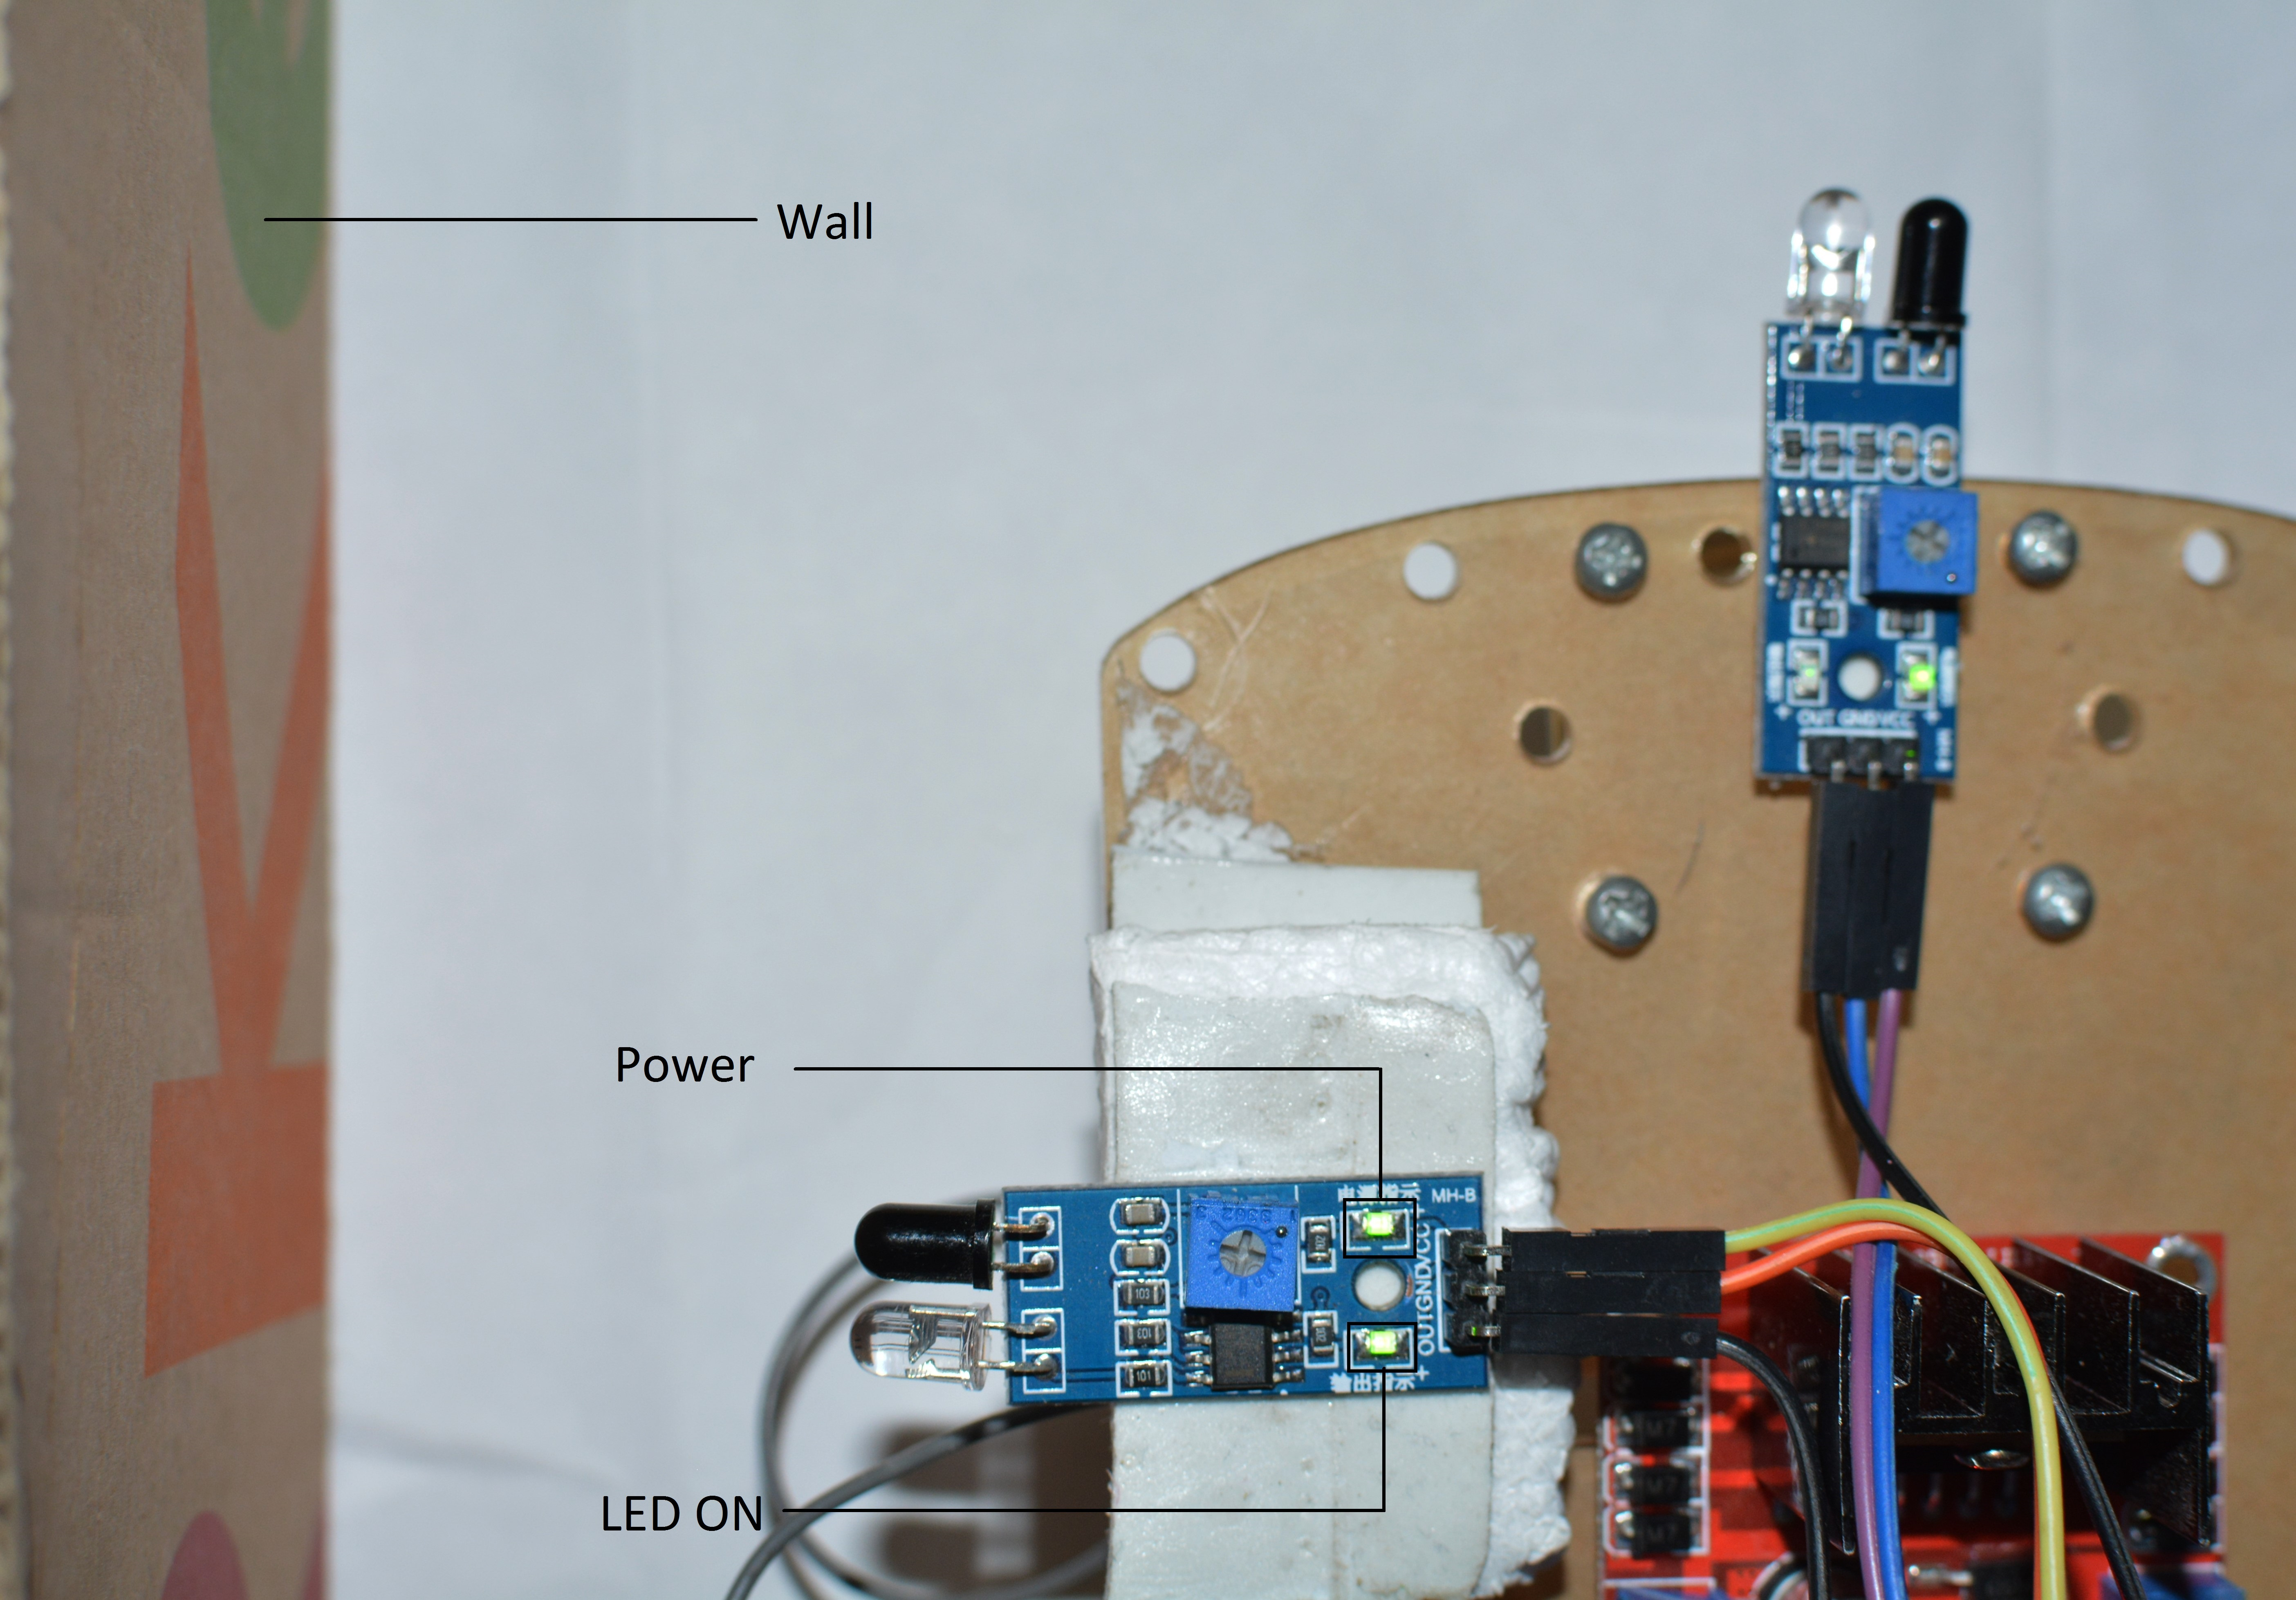
\includegraphics[scale=0.21]{part3_1_lb.jpg} 
                \caption{The detection of wall by the left sensor}
                
        \end{subfigure}
        \begin{subfigure}[b]{0.5\textwidth}
                  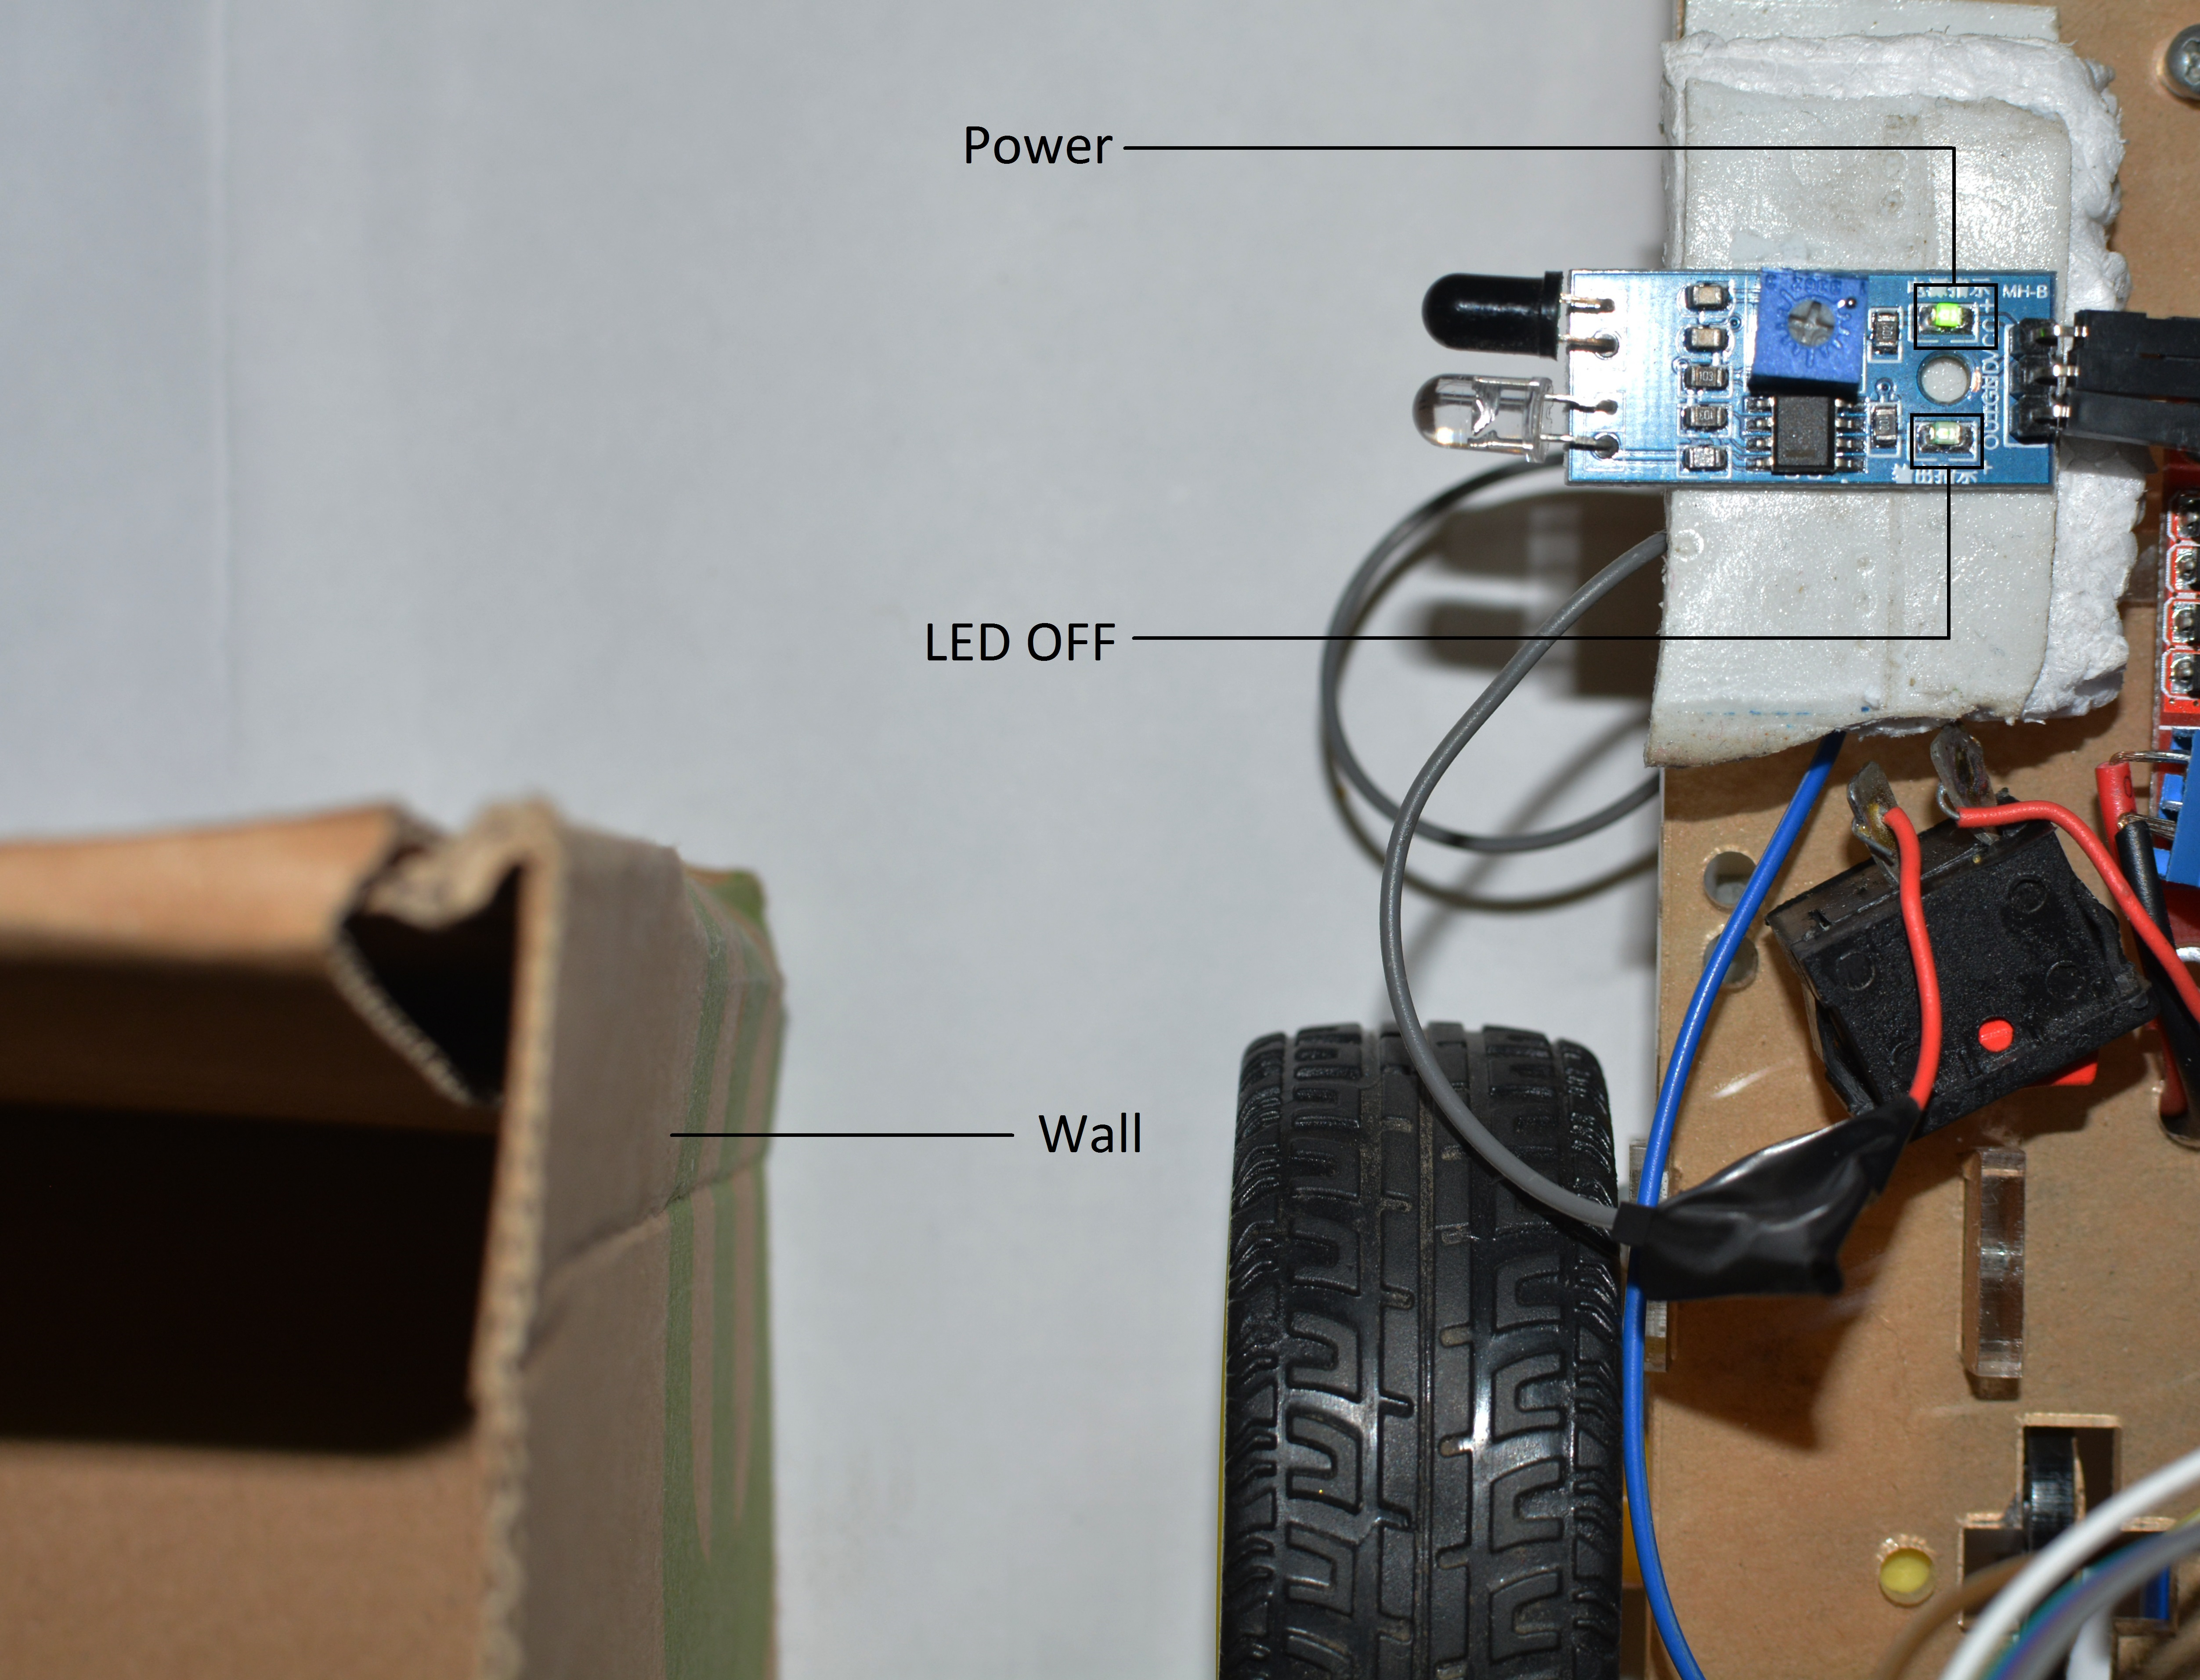
\includegraphics[scale=0.21]{part3_2_lb.jpg} 
                \caption{No detection of wall}
                \label{fig:gull2}
        \end{subfigure}%
        \caption{Implemenation of the IR sensor for detection of the left wall}
\end{center} 
\end{figure}
\justify Similarly, the following image shows the working of the IR at different distances from the front of the wall.\\
\newpage
\begin{figure}[h]
\begin{center}
        \begin{subfigure}[b]{0.5\textwidth}
                 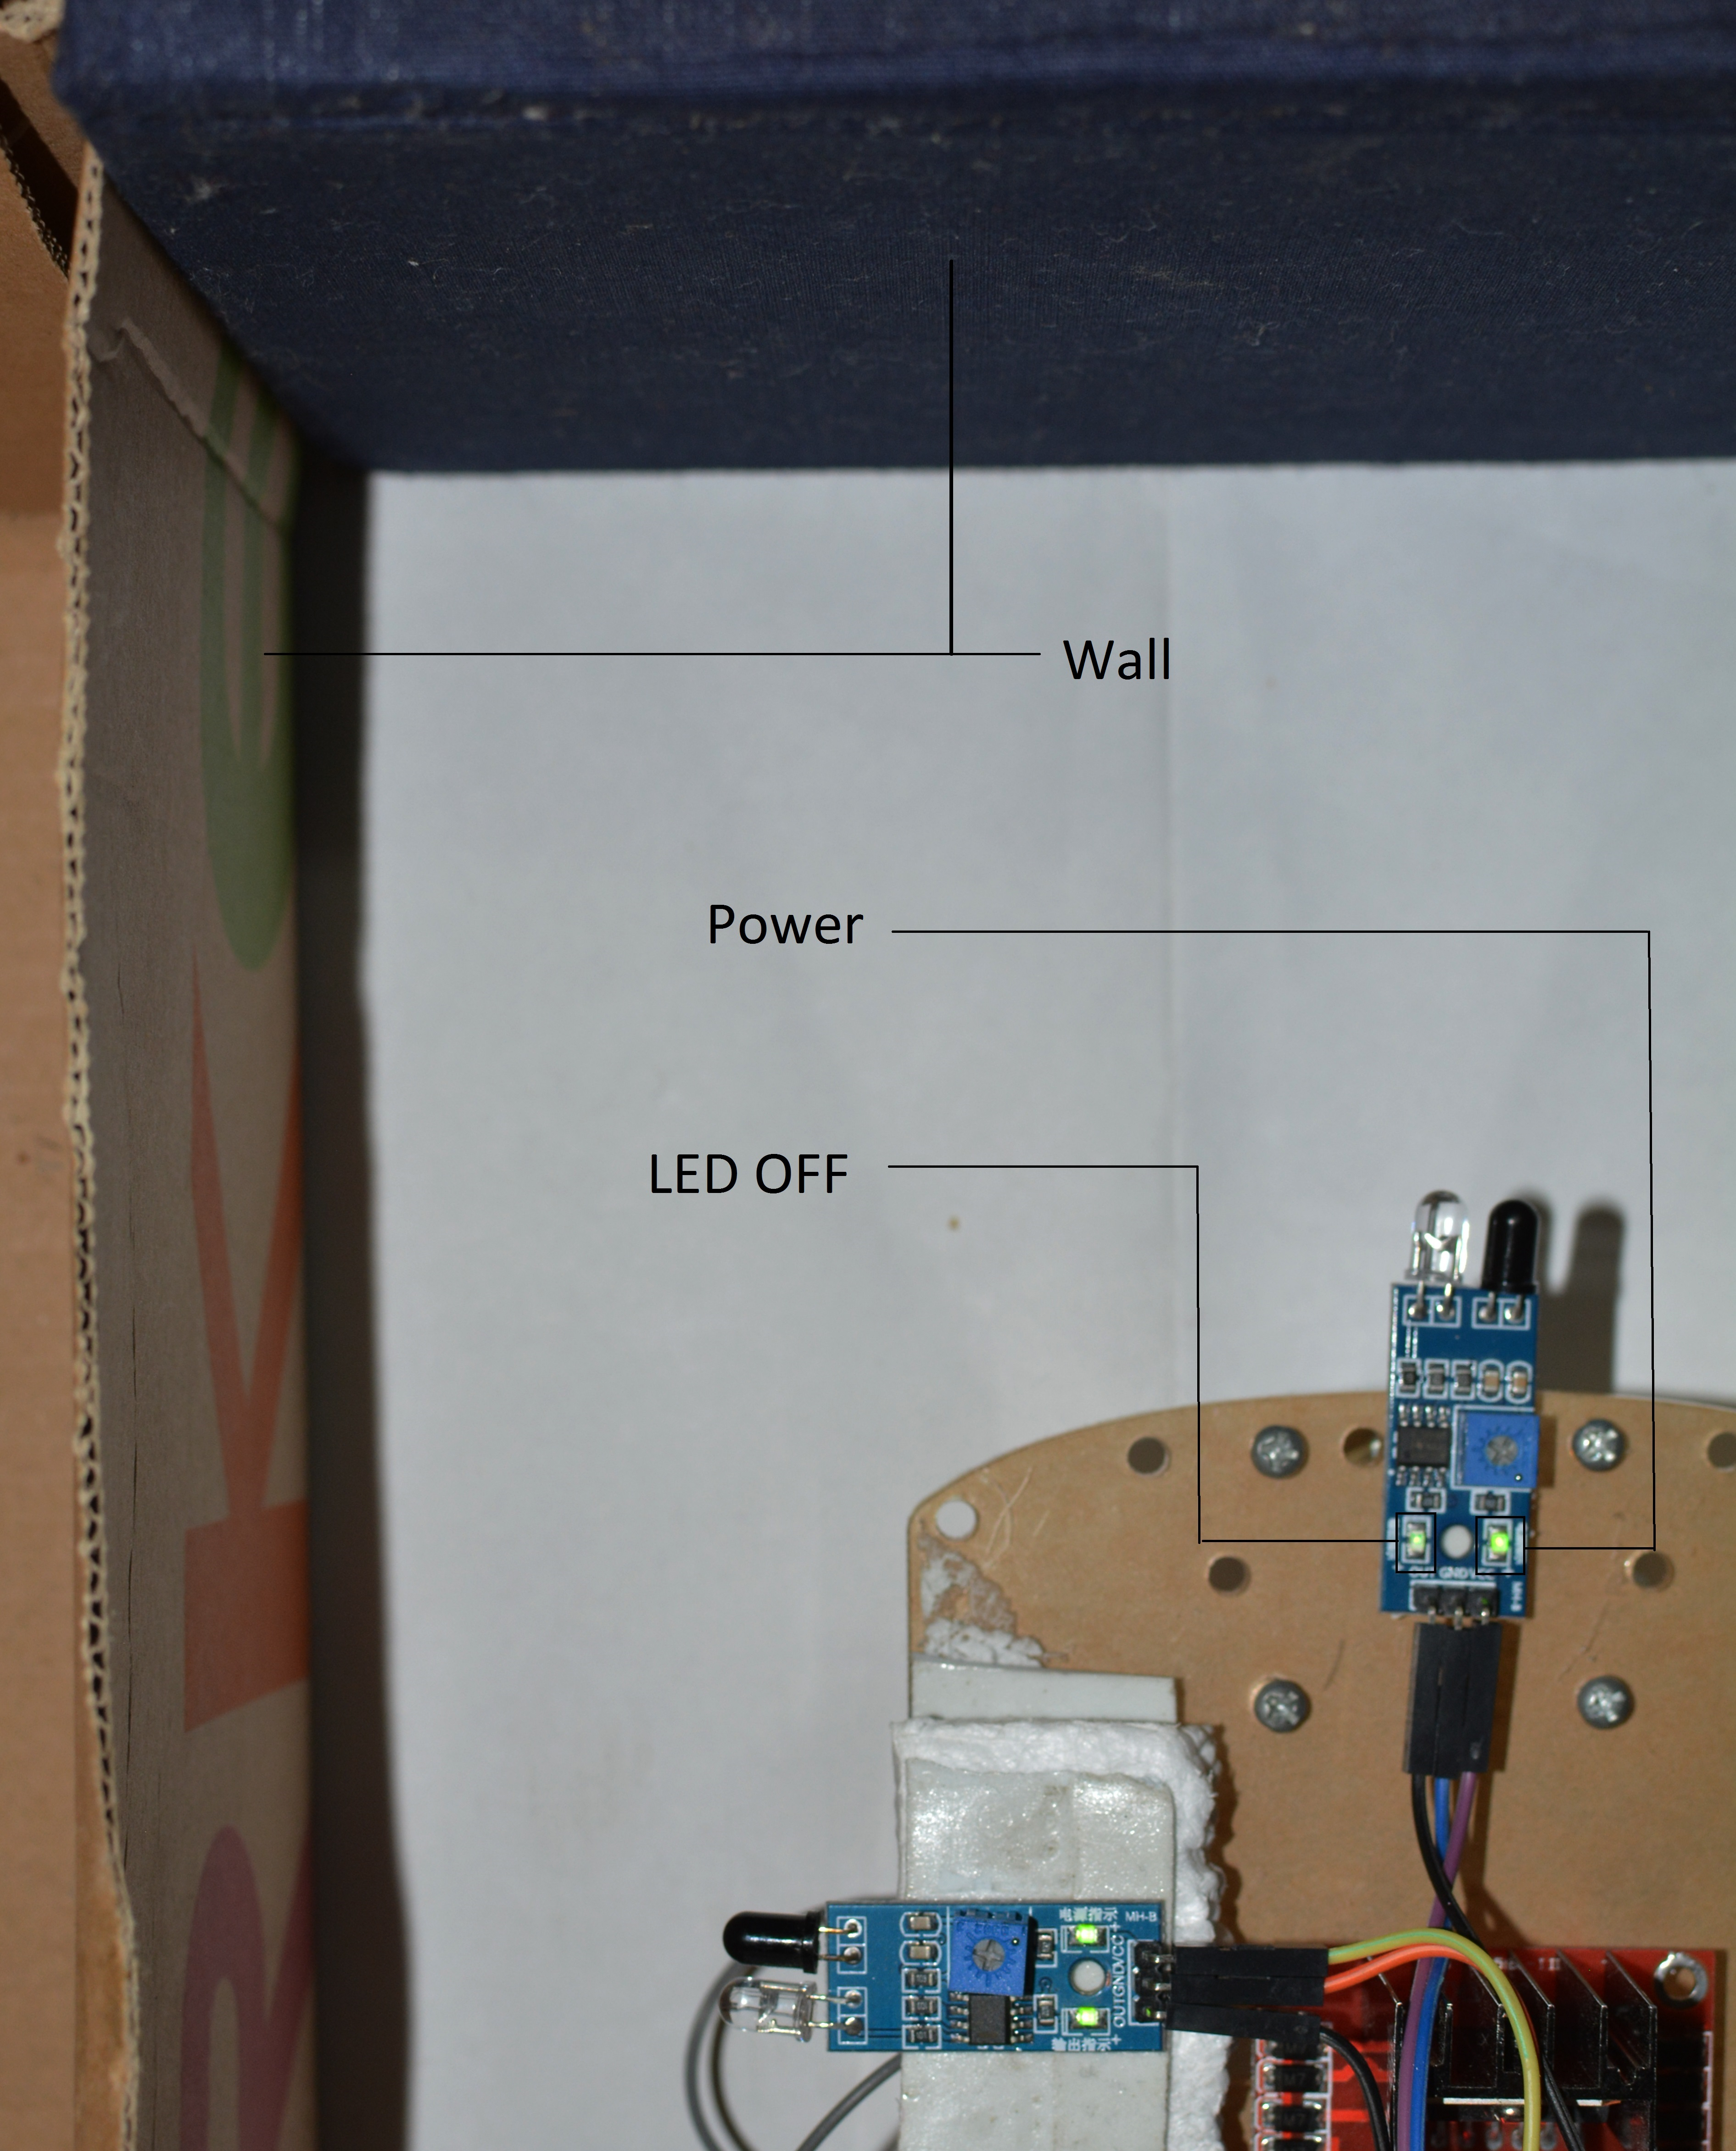
\includegraphics[scale=0.195]{part3_3_lb.jpg} 
                \caption{No detection of wall by the front sensor}
        \end{subfigure}
        \begin{subfigure}[b]{0.5\textwidth}
                  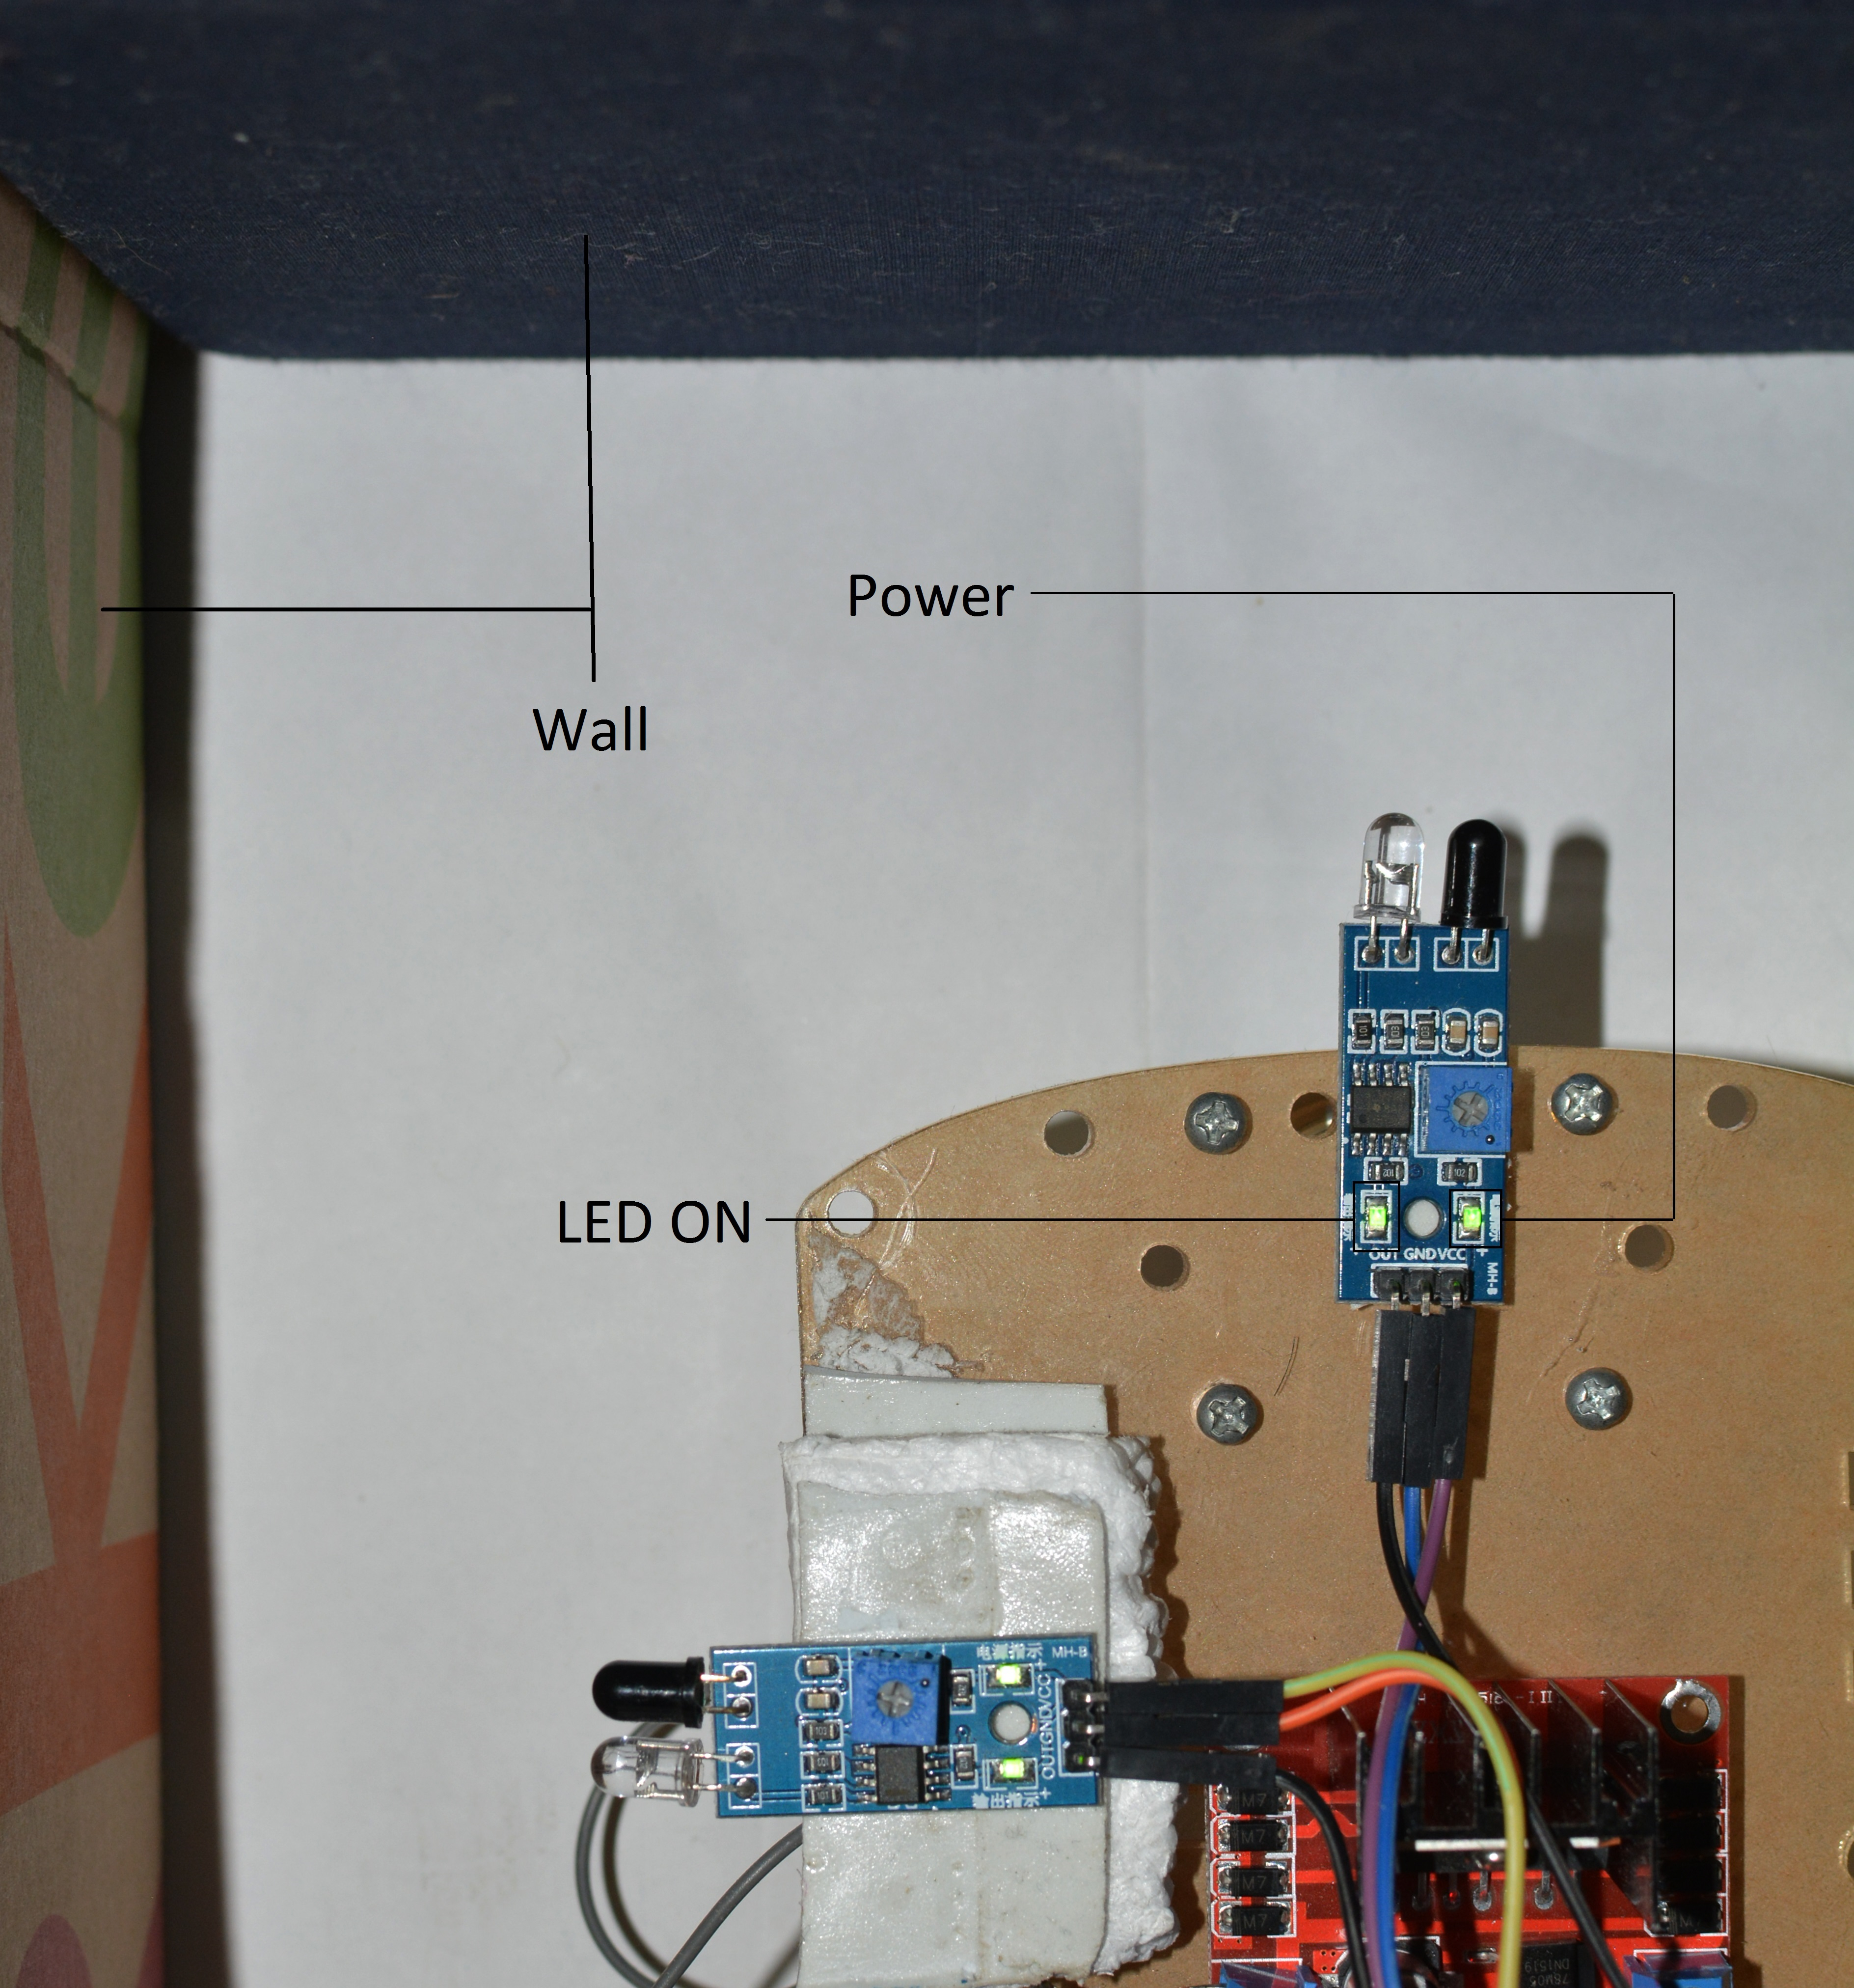
\includegraphics[scale=0.195]{part3_4_lb.jpg} 
                \caption{Detection of wall by the first sensor}
                
        \end{subfigure}
        \caption{Implemenation of the IR sensor for detection of the front wall at different distances}
\end{center} 
\end{figure}
\subsection{Path traversal by the second robot}
The second robot received the information/decision from the first robot and started traversing the maze. The junction in the maze was detected by a set of IR Sensors similar to that on the first robot.  Upon the arrival of the junction ,  the second robot took the desired decision that led the robot through the shortest path to the target.\\
Based on the above example, the result is shown below as: \\
Firstly, the second robot was placed at the initial position similar to as that of the first robot.
\begin{figure}[h]
\center
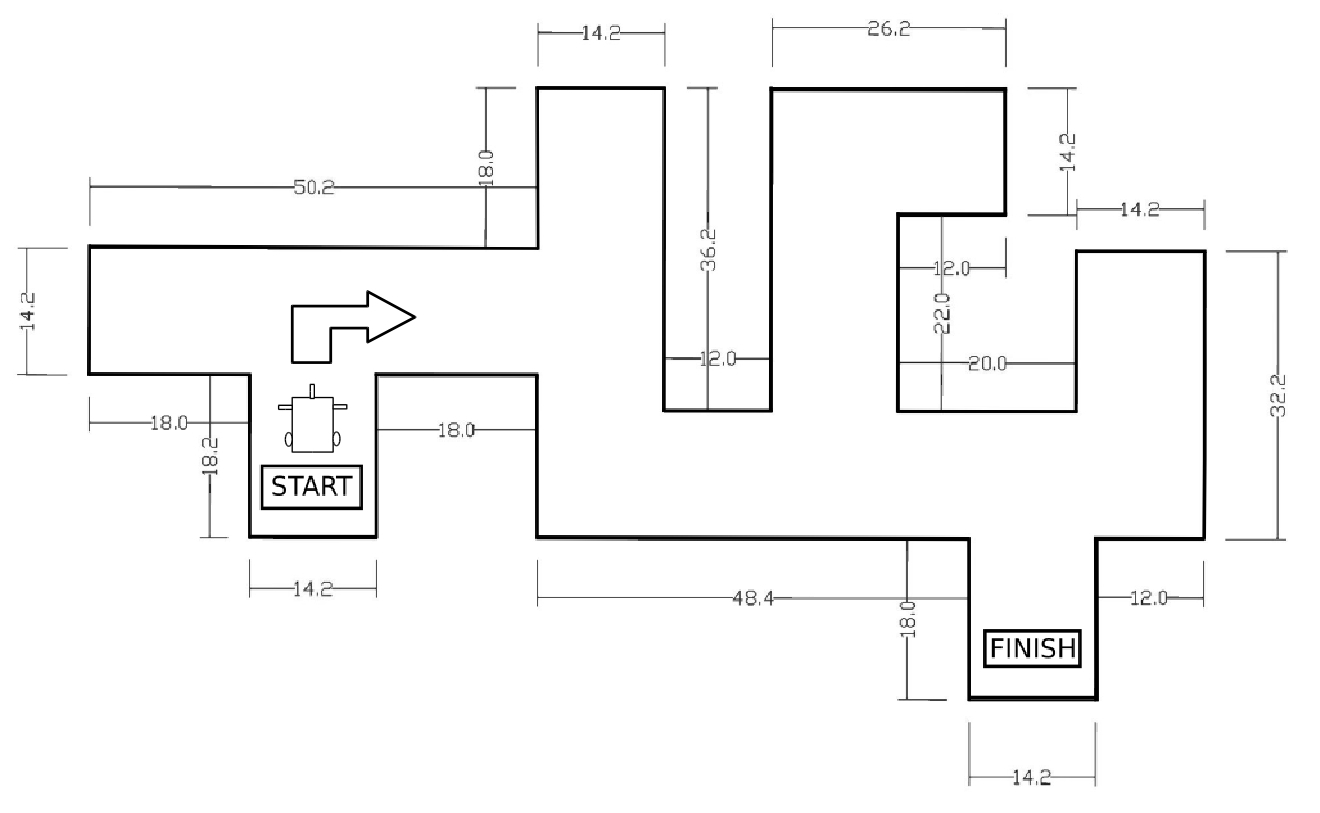
\includegraphics[scale=0.35]{part1_4new.jpg} 
\caption{Initial placement of the second robot similar to that as of the first robot}
\end{figure}
\justify Based on the left wall following algorithm, the first robot took the decision of following the left wall as shown earlier in the\ref{Firstplacementofthebot} Here, the second robot took the decision to go right based on the decoded packet sent by the first robot for reaching the target through the shortest path.\\
The robot movement continues through the shortest path throughout the maze all based upon the decoded packet.\\
\newpage
\begin{figure}[h]
\center
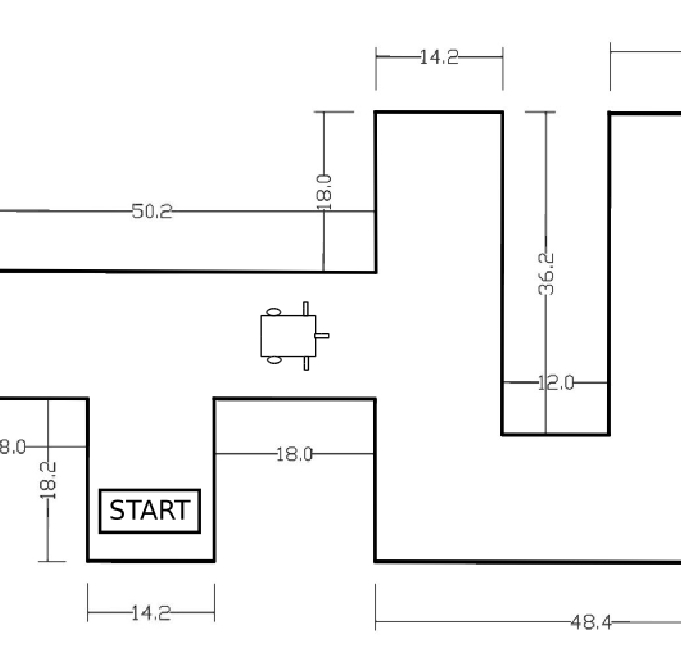
\includegraphics[scale=0.32]{part1_5new.jpg} 
\caption{Robot locomotion continues via the shortest possible path}
\end{figure}
\justify
On following the route provided by the first robot, the second robot ultimately reached the target.\\
\begin{figure}[h]
\center
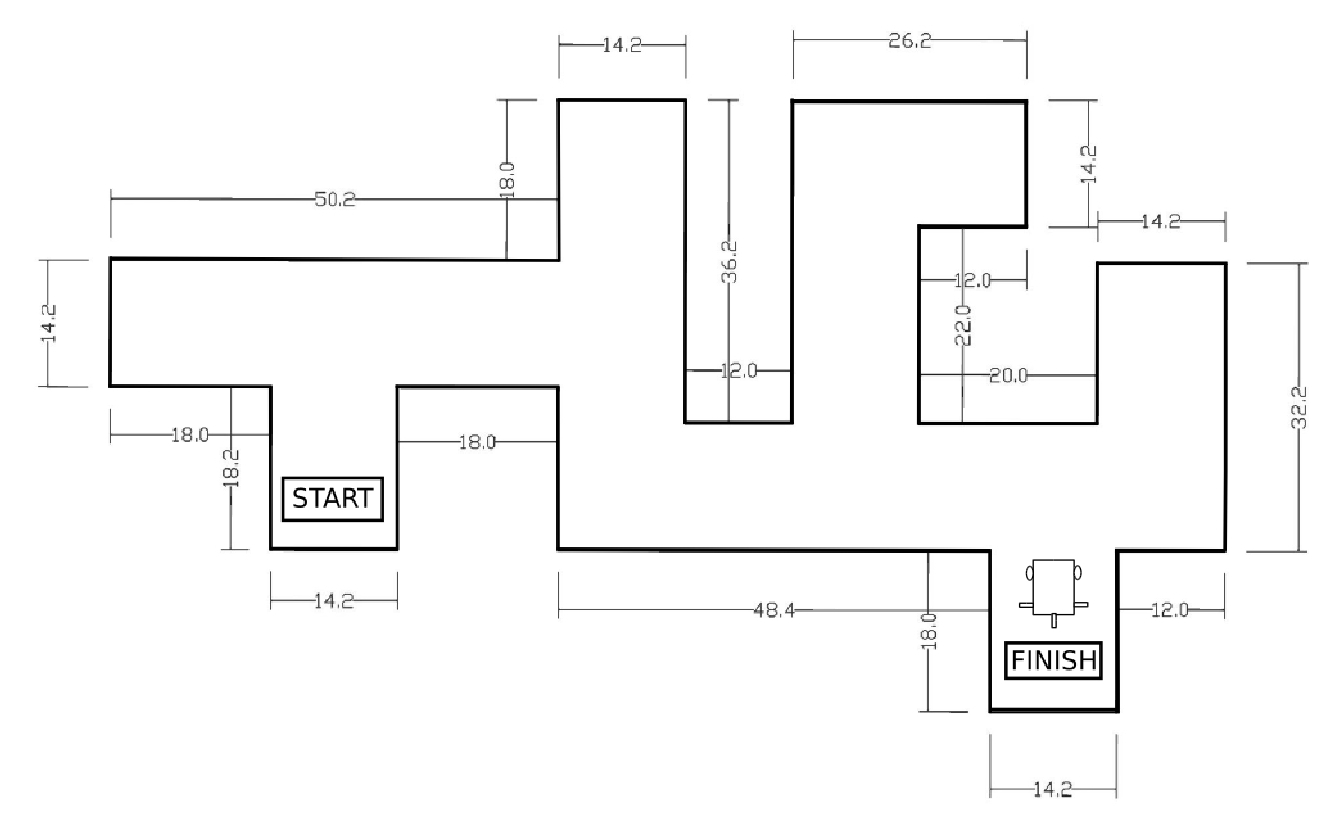
\includegraphics[scale=0.25]{part1_6new.jpg} 
\caption{Reaching of the target}
\end{figure}
\justify Thus, the route for the shortest path was obtained and implemented by the second robot successfully.
\subsection{Bluetooth Communication}
All the decisions required for solving the maze in the most efficient way were stored in a queue by the first robot which was then sent to the second robot via HC-05 Bluetooth module.\\
\begin{figure}[h]
\center
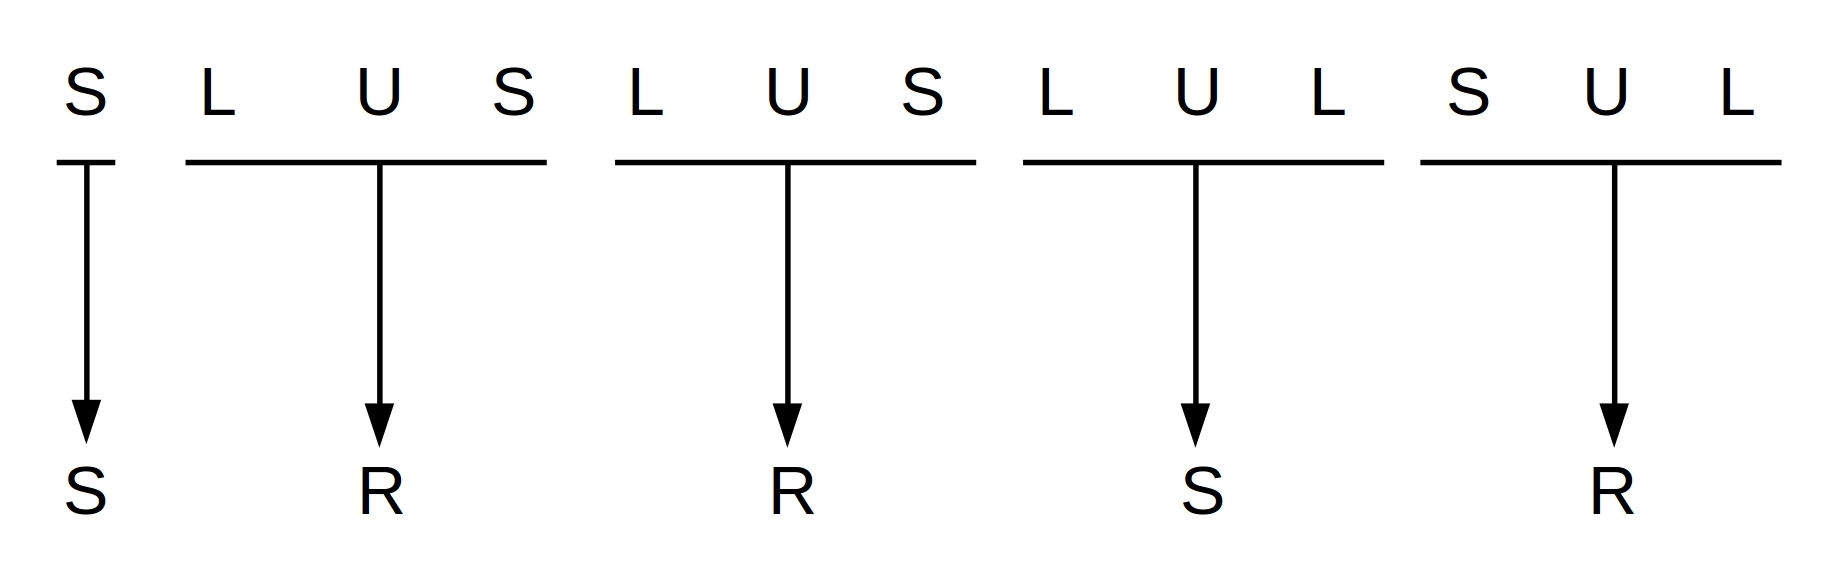
\includegraphics[scale=0.2]{decoding.jpg} 
\caption{Decoding Algorithm}
\end{figure}
\justify The figure above shows the decoding process of the junction decisions carried out by the first robot. This process is a \textit{"reduction process"} where the decisions taken by the first robot at respective junctions of the maze were re-examined and a more optimal result was extracted. The second robot traversed the maze according to this decoded packet of information and was able to reach the target through the shortest path possible.\\
The underlying algorithm behind this reduction process is to look for the occurrence of a U-turn (denoted by 'U'). For every occurrence of a U-turn, the robot adds the opposite decision that it took at the last junction  to the queue.\\
For example, if the robot reached a junction where it could go either left, (L) or drive straight (S)  it would turn left. But if it encountered a U-turn after taking the left turn, the opposite decision in the last junction i.e. straight, (S) would be added to the queue. \\
From the figure shown below, it can be seen that when the first robot encounters a U-turn for the first time, the decision not taken at the first junction is entered into the queue. So, the decisions L U S is replaced by R. \\
Similarly, the remaining occurrences of U-turns were decoded using this technique wherein L U L was converted to S and S U L to R. This way, the final junction decisions for the shortest path was extracted.\\
\begin{figure}[h]
\center
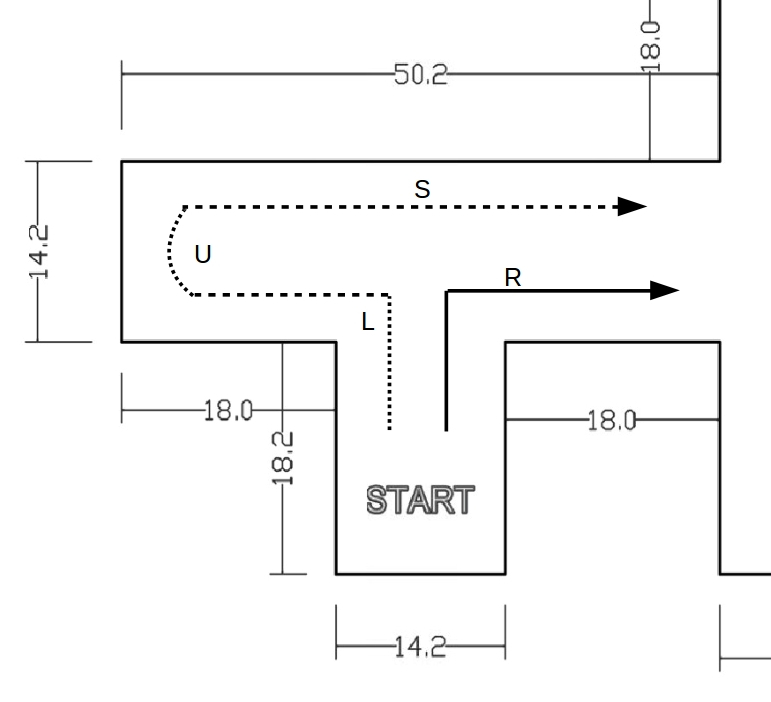
\includegraphics[scale=0.5]{deconding_1_final.jpg}
\caption{Implementation of \textit{reduction process}} 
\end{figure}
\subsection{Motor Synchronization}
Various problems and shortcomings were faced during the course of the progress of the project.However, most of them were overcome.\\
One of the first shortcoming was the synchronization of the two motors. Even though the two motors were identical in terms of specifications and manufacture, like all devices, they had inherent differences. As a result, the rate of rotation of the two motors were different and the bot failed to move in a perfectly straight line. This problem can be solved by using a closed control circuit, most probably using IR sensors to make a P-control system.
\subsection{Operation of Wheel}
Another shortcoming was the front wheel to be used in the robot. At first, a roller wheel was used  but with the rotation of the robot, the roller wheel rotated as well which changed the center of the weight of the robot thus hampering it's forward movement which resulted in non-uniform movement of the robot.\\
This shortcoming was overcomed with the use of the caster wheel. The use of caster wheel removed the problem of shifting of center of weight thus resulting in uniform motion.
\subsection{IR Sensors}
Another problem was the accuracy of the IR sensor module. Initially, various IR modules were tested to check the accuracy and distance up to which they operated. Most of them failed to correctly detect the maze walls at the proper distance. Hence, the modules used currently was the one selected to be used in the bot both in terms of accuracy and economy.\\
The IR transceiver pair was able to detect the obstacles i.e. the walls of the maze with the help of the reflection of the IR signals transmitted by the IR transmitting diode which were detected by the IR receivers. The potentiometer was used to adjust the resistance to one of the pins of the FC-51 which allowed us to adjust the sensing distance for the sensor.
\subsection{Power Source}
Selection and finding the best Li-Po battery of the required voltage and current specification was a daunting task and a 7.4v 1600mAh battery was selected as the most suitable choice. The Li-Po battery has a voltage rating of 7.4V. The output from this battery is provided to the L298N motor driver whose 5V output is used to drive the Arduino board. The 5V output from the Arduino Board is used to power the IR sensor module. \\
The output current capacity from the 5V output pin of the Arduino is ~500mA. According to the IR sensor module specification, the maximum current rating of each module is around 43mA when operating at 5V. Performing required calculations, four such sensors can be easily accommodated from the pin output of the board. \\
Furthermore, the connection of the Arduino to the motors was challenging in the sense that the output pins inherently had different clock frequencies and this resulted in the wheels rotating at different speeds. 
\subsection{PWM Generation}
The PWM signal was generation from microcontroller (ATMEGA 398). The H-Bridge was a interface between the microcontroller and DC motor. Using H-Bridge, the circuit was prevented from bursting. The battery would have to be inverted time and again if H-Bridge hadn't been used. The upper waveform is for Motor 1 and the lower one is for lower Motor 2 in all the figures shown in the result section. Motor should have stopped if same signal were passed to all the transistor of H-Bridge and same is the principal we have used for stopping the motor. The clockwise motion , anticlockwise motion and no motion was observed respectively. Between each clockwise and anticlockwise motion, delay of 3 seconds was observed.\\
\begin{figure}[h]
\center
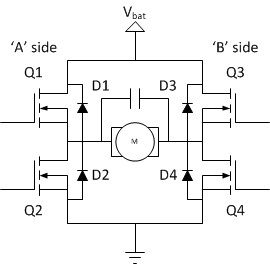
\includegraphics[scale=1]{hbridge.jpg} 
\caption{Diode configuration in H-Bridge}
\end{figure}
\justify The diodes (D1..D4) are called catch diodes and are usually of a Schottky type. Diode is basically a two-terminal electronic component that conducts primarily in one direction (asymmetric conductance). We need diodes for circuit to work. Without diodes, rest of the H-bridge gets killed at the moment motor turns off.\\
There are two types of elements that store energy: capacitors and inductors. Capacitors store charge because the energy can be stored statically.\\
Inductors cannot store energy statically. When circuit opens, they deliver that energy regardless if circuit is ready for it or not. Inductors are like railroad train which takes time to accelerate but it takes time to stop it. It does not stop instantly.  Inductors takes time for current flow through it to grow, but when the circuit is turned off, current does not stop instantly (even though you have open circuit). Inductor will keep on pushing that same current through whatever resistance that 'open circuit' is. Eventually voltage builds up until there is an insulation breakdown. If the insulator is air, we can see the spark. In case of H-Bridge, sparks are inside transistors.\\
So, we need diodes to divert running train to an alternate track so it has time to slow down, i.e, provide the path for the inductive "kick" that is generated when the motor is switched off in h-bridge circuit. Also, the diodes prevent back EMF when the motor is switched off.\\
For this, IN1 and IN4 were set high and IN2 and IN3 were set low. So, the current moved from IN1, through motor and then to IN4 of H-Bridge. As both EN1 and EN2 were given more than half the maximum value of PWM, both their waves are same. Even when the PWM value was changed, there was only the small change in waveform. The duty cycle here was 60 percent.  When the maximum value of PWM was given, the waves weren’t visible because the speed was too high. The current is flowing from the top left to buttom right in this case without flowing through IN2 and IN3. \\
Here, contrary to the case of clockwise direction, IN2 and IN3 were set high (1) while IN4 and IN5 were set low (0). The duty cycle here was 60 percent. The waves are narrower than that of the clockwise direction. In between clockwise and anticlockwise, delay of 100 ms was taken so that the motor may not have the chance of crashing on changing direction abruptly. The current is flowing from IN2, through the motor and to IN3, i.e, it is flowing from buttom left to top right.\\
In the case of leftward, pins IN1 and IN3 were set low while the remaining pins were high. The current thus moved from buttom left to buttom  right crossing the motor. IN 2 and IN 4 were given high, i.e, 1. The PWM values in this case were also the same as clockwise and anti- clockwise direction so, duty cycle was also the same, i.e, 60 percent. The wave of motor 1 is narrower like anticlockwise motion while in motor 2, the waves are wider like of clockwise motion.\\
For the rightward motion of the robot, IN1 and IN3 were set high, i.e, 1 and the remaining pins were low. The PWM value to ENA and ENB and also the duty cycle was same in this case too. The current here thus moved from top left to top right through the motor. If the direction had been reverse, the motor would have moved in left direction. Here, the wave of Motor 1 is wider like clockwise and Motor 2 has narrower wave like anticlockwise contrary to left sided motion.\\




\newpage
\section{CONCLUSION}
Thus, we were able to successfully meet the desired objectives of the project within the given time period. Some minor shortcomings were experienced and were successfully tackled.  
\subsection{Limitation} 
The objectives specified initially was completed in the given time and with the available resources with some minor changes along the development process. The project still has some limitations which are to be solved in future revisions. They are as listed below: 
\begin{enumerate}
\item The accuracy of the IR sensors was very less and produced erroneous results when directly subjected to sunlight, requiring a closed room to function properly.
\item Use of R sensors makes the robot incapable to trace the map of the maze that it traverses.
\item The bluetooth module HC-05 cannot be used for establishing connection between more than two robots. 
\item Use of wall follower algorithm to solve the maze limits the structure of the maze to be simple connected (i.e. all its walls are connected together or to the maze's outer boundary).
\end{enumerate}
\subsection{Future Enhancement}
The enhancements to be implemented in the project to overcome the limitations stated above as well as to provide advanced features are as follows:
\begin{enumerate}
\item Use of robust IR sensors that work under a variety of light conditions and be able to detect the distance from the obstacles.
\item Integration of a camera with the robots to map the maze surrounding and implement dynamic path planning.
\item Using IEEE 802.11 protocol in the system in order to implement more than two robots in the maze.
\item Implementing a stronger algorithm to make all the robots scan and traverse the maze at the same time simultaneously.
\end{enumerate}
\subsection{Recommendations}
This project is a demonstration of the concept of swarm robotics in task solving and can be applied to various applications. The project uses two robots to solve a maze and can be used in disaster zones where it is dangerous for humans to undertake the rescue operation like search and rescue operations (SAR). It can also be used in traversing an unknown environment where the target location is not determined such as in hostage rescue situations. By prevailing over the existing
limitations, it can be used for land-mine detection where one robot detects the land-mine and the other robot goes to the location to diffuse it.

\newpage
\bibliographystyle{IEEEtrans}
\bibliography{final_reference}
\newpage

\end{document}